\documentclass{article}
\usepackage{graphicx}
\usepackage{wrapfig}
\usepackage{subcaption}
\usepackage[margin=1in]{geometry}
\usepackage{amsmath} % or simply amstext
\usepackage{siunitx}
\usepackage{booktabs}
\usepackage[export]{adjustbox}
\newcommand{\angstrom}{\textup{\AA}}
\usepackage{cleveref}
\usepackage{booktabs}
\usepackage{gensymb}
\usepackage{float}
\usepackage{setspace}
\usepackage{color}
\doublespacing

\title{Understanding the nanoscale structure of hexagonal phase
lyotropic liquid crystal membranes}
\author{Benjamin J. Coscia \and Douglas L. Gin \and Richard D. Noble
\and Joe Yelk \and Matthew Glaser \and Xunda Feng \and Michael R.
Shirts} 

\begin{document}

  \bibliographystyle{ieeetr}
  \graphicspath{{./figures/}}
  \maketitle

  \begin{abstract}

  Nanostructured porous membranes made from the cross-linked hexagonal phase of
  self-assembled lyotropic liquid crystals (LLCs) are a promising material for
  selective separations. To date, their separation performance has only been
  characterized with membranes made from a small set of LLC monomers. There
  remains a large design space that we can likely exploit to design membranes for
  solute specific separations. In this work, we develop an atomistic molecular
  model of an LLC membrane. We show that our model is maximally consistent with
  experimental observations by comparing simulated X-ray Diffraction (XRD)
  patterns and calculated ionic conductivity to their experimental counterparts.
  We explore, in depth, the composition and structure of the nanopores in order
  to give insights that are not easily accessible to experimentalists. With the
  clear picture of the nanoscopic structure of these membranes gained from this
  work, we will be able to use the model to understand the mechanisms of small
  charged and uncharged solute transport within the nanopores, and eventually we
  will be able to screen large sets of modified monomers with their separation
  properties in mind.  

  \end{abstract}

  \section{Introduction}
  
  Reverse osmosis (RO) and nanofiltration (NF) are membrane based separation
  processes widely used to create potable or reusable water by removing salts and
  other dissolved compounds from water sources. RO membranes are typically thin
  film composite (TFC) membranes with a porous support layer and a dense
  crosslinked polymer active layer which near indiscriminately separates all solutes.
  NF membranes are porous with pores on the order of 1 $\nm$ in size which separate 
  primarily based on solute size.   

  RO and NF are finding applications beyond primarily water-based
  separation. Recovery of valued products from complex aqueous and organic waste
  is of increasing interest. This requires highly selective membranes.

%  The permeability-selectivity tradeoff is a well-known problem in the membrane
%  separations community. It is difficult to increase the permeability of a 
%  desired molecular or atomic species, while maintaining the same retention of
%  an undesired species.

%  Current commercial RO and NF membranes suffer from limitations inherent to
%  their fabrication. Although scalable, each of these two types of membranes has
%  a degree of stochasticity that makes overcoming the permeability-selectivity
%  tradeoff a challenge. Namely, it is difficult to increase the permeability of
%  a desired molecular or atomic species, while maintaining the same retention of
%  an undesired species \cite{werber_materials_2016}. 
 
  Selective separation by a semipermeable membrane barrier is governed by two
  steps : barrier entry and transport through the barrier. A solute's ability to
  enter a membrane barrier is decided by its size, solubility and charge. A solute's
  size, shape and polarity affect its ability to travel across the barrier. Undesired
  solutes may still be able to enter the membrane making their diffusion rates
  relative to desired solutes important. It is important to design the membrane in response
  to desired and undesired solutes is thus important. 

  NF -- pore polydispersity
  RO -- r0andom walk through polymer voids

  Nanostructured porous membrane materials have become increasingly popular for
  aqueous separations applications such as desalination and biorefinement because
  they offer the ability to control pore architecture at the molecular scale,
  thereby permitting the design of solute-specific separation membranes
  \cite{humplik_nanostructured_2011}. One can acheive most membrane-based aqueous separations of
  small molecules using reverse osmosis (RO) or nanofiltration
  (NF) \cite{van_der_bruggen_review_2003}. While RO and NF have seen many
  advances in the past few decades, they are far from perfect separation
  technologies. 

   %MRS4: these two paragraphs are perhaps not ideal.  They describe the process
  %of making the membranes, but that is not what we need as the introduction to
  %THIS paper.  Instead, you need to focus on the strength/issues with RO and
  %NF that motivate this research.
  % BJC3: The point I am trying to make is that the way the membranes are made 
  % results in either low selectivity or low permeability. I could just state
  % that, or give a little background on the processes to make the point more
  % tangible

  Commercial RO membranes are typically dense thin-film composite (TFC)
  membranes with a porous support layer and an active layer made of a polymer
  matrix formed through interfacial polymerization \cite{jeong_interfacial_2007}.
  During interfacial polymerization, a step-growth polymerization reaction occurs
  at the interface of an aqueous monomer solution that has been soaked into the
  support layer, and an organic solution of a second monomer. The polymer matrix
  is dense and highly cross-linked which gives high rejections but low
  permeability. 

  %During membrane fabrication,
  %aqueous diamine solution is allowed to penetrate into the polysulfone support
  %layer which is then immersed in trimesoyl chloride, a compound that is
  %immiscible in water. Diamine polymerizes with trimesoyl chloride at the
  %solution interface and creates a thin film that physically adheres to the
  %polysulfone support. 
 
%  solution.  Through the use of a non-solvent, a polymer-rich and polymer-poor
%  phase is formed. A membrane is created as the polymer-poor phase forms pores in
%  the polymer-rich phase. 
%  During phase inversion, a thin polymer film is precipitated out of a polymer
  NF membranes are typically porous membranes made by a phase-inversion
  process. The most widely used phase-inversion process is immersion
  precipitation, during which one submerges a polymer, dissolved in a solvent, in
  a non-solvent. A solid, porous polymer membrane is all that remains once all
  solvent has been removed by non-solvent exchange
  \cite{smolders_microstructures_1992}.  The resultant pores are polydisperse in
  size, which hurts membrane selectivity. A second technique used to create NF
  membranes is call track-etching in which a polymer film is bombarded with
  charged particles, then chemically etched to create pores
  \cite{apel_track_2001}. The pores are uniform, which benefits selectivity;
  however, the membranes have a low porosity and subsequently low permeability. 
 
%MRS3: this is a little disconnected to the contents as well.  You want
%the paper to explain the why of doing this research.  Paragraph gives background, but doesn't motivate. 

%  Current commercial RO membranes are thin film composite membranes with a
%  porous support layer and an active layer made of a dense polymer matrix. The
%  membranes are unstructured with tortuous and polydisperse diffusion pathways.
%  Separation occurs based on differences in solubility and diffusivity of solutes
%  within the polymer matrix \cite{wijmans_solution-diffusion_1995}. With
%  optimization, one can exploit these differences to create a functional
%  selective barrier. RO operation costs are suboptimal because high feed
%  pressures are required in order to achieve a useful solvent flux. 

  %BJC : I don't know that this paragraph fits.  
  %MRS3: not really. Maybe take a look at Osuji's recent review (2016, I think) that addresses applications of nanostructured membranes and uses.  Could rewrite the introduction to be more about the general possibilities of nanostructured membranes, not just desalination.  It should be an introduction to what you will talk about in the paper, not to everything related.
 % Improved RO membranes can make desalination more sustainable. Only 0.5\% of
 % the world's water is fresh. Desalination is an important source of potable
 % water, necessary in order to keep up with demand generated by a rapidly growing
 % global population. Although RO is currently the cheapest form of desalination,
 % the cost must be further decreased in order to meet demand. A typical seawater
 % desalination process requires feed pressures in the range of 800 to 1000 psi
 % \cite{fritzmann_state---art_2007}. By designing better membranes for
 % desalination, we can achieve higher water fluxes and reduce feed pressure
 % requirements which will decrease the cost of fresh water production.
 % \cite{humplik_nanostructured_2011}.  

  % financially straining developing regions and contributing strongly to
  % CO\textsubscript{2} emissions. \cite{mcginnis_global_2008} Moreover,
  % designing RO membranes to achieve targeted separations of specific solutes
  % in a complex feed solution is nearly impossible

  %NF was introduced as an intermediate between RO and ultrafiltration, having
  %the ability to separate organic matter and salts on the order of one nanometer
  %in size. Explicit pore pathways running through the thickness of the membrane
  %permit high solvent fluxes at lower pressures than RO. NF membranes typically
  %have a surface charge resulting from ionizable groups which affords separation
  %of ions smaller than the pore radius by the mechanism of Donnan exclusion
  %\cite{van_der_bruggen_review_2003}. NF is often used as a precursor to reverse
  %osmosis since it can efficiently remove a significant portion of dissolved
  %solutes. Following NF pretreatment, RO can further purify the permeate. 
  %Unfortunately, NF membranes, like RO, possess a pore size
  %distribution which limits their ability to perform precise separations
  %\cite{bowen_modelling_2002}. 

  The permeability-selectivity tradeoff has the potential to be overcome by
  designing membranes at the molecular level. Next-generation nanoporous
  membranes with high selectivity, permitted by a precisely controlled pore size,
  and high permeability, allowed by its porous architecture, have the potential to
  replace traditional RO and NF membrane technologies. 

%MRS3: I think that this paragraph probably should be couched in terms of what they COULD do, since are not widely used yet.
%MRS3: if talking about existing membranes, should cite performance.
%  Nanostructured membranes can bypass many of the performance issues which
%  plague traditional NF and RO membranes. One can accomplish targeted separations
%  with high selectivity by tuning shape, size and functionality of the molecular
%  building blocks which form these materials. As a result, solute rejecting pores
%  can have their sizes tuned uniformly, resulting in strict size cut-offs.
%  Entirely different mechanisms may govern transport in a given nanostructured
%  material which can inspire novel separation techniques.

  Development of nanostructured porous materials has been limited by the
  ability to synthesize and scale various fundamentally sound technologies.
  Graphene sheets are atomically thick which results in excellent water
  permeability but defects during manufacturing severely impact selectivity
  \cite{cohen-tanugi_multilayer_2016}. Molecular dynamics (MD) simulations of
  carbon nanotubes show promise \cite{humplik_nanostructured_2011}, but synthetic
  techniques are unable to achieve scalable alignment and pore monodispersity
  \cite{hata_water-assisted_2004,maruyama_growth_2005}. Zeolites have sub-nm
  pores with a narrow pore size distribution, and MD simulations of these
  materials show that they exhibit complete rejection of solvated ions
  \cite{murad_molecular_1998}- however, experimental rejection was low and
  attributed to interstitial defects formed during membrane synthesis
  \cite{li_desalination_2004}. Consequently, there is a need for a scalable
  nanostructured porous membrane. 

  Polymeric membranes based on self-assembling lyotropic liquid crystals (LLCs)
  are suitable candidates for aqueous separation applications. LLCs are
  amphiphilic molecules that share the characteristic ability of nanostructured
  porous membrane materials to create highly ordered nanostructures with the
  added benefits of low cost and synthetic techniques feasible for large-scale
  production \cite{feng_scalable_2014}. LLC systems created by the monomer
  Na-GA3C11 (Fig.~\ref{fig:monomer}) have been extensively studied experimentally
  \cite{feng_scalable_2014,smith_ordered_1997,zhou_supported_2005,resel_h2-phase_2000,feng_thin_2016}.
  The neat Na-GA3C11 monomer forms the thermotropic liquid crystalline (TLC)
  Col\textsubscript{h} phase (Fig.\ref{fig:assembly}). The presence of ca. 10
  wt\% added water results in formation of the lyotropic H\textsubscript{II}
  phase. In both cases, Na-GA3C11 monomers assembles into mesophases made of
  hexagonally packed, uniform size, cylinders with hydrophilic head groups
  oriented inward towards the cylinder center. This LLC assembly is then
  polymerized in situ to form a cross-linked polymer network to stabilize the
  structure. The hydrophilic region can act as a pore for aqueous separations
  \cite{zhou_supported_2005}.  One can envision tailoring the pore region for
  specific separations by changing the monomer chemistry
  \cite{resel_h2-phase_2000}.

  Research into polymerized LLC membranes has been revived in recent years.
  During early stages of exploration, mesophases formed by Na-GA3C11 could not be
  macroscopically aligned, resulting in low flux membranes, and no clear route
  towards scalable and economical filtration. In 2014, Feng et al.~showed that
  one can align the mesophases using a magnetic field with subsequent
  cross-linking to lock the structure in place \cite{feng_scalable_2014}. In 2016,
  Feng et al. showed that one could obtain the same result using a second
  technique termed soft confinement \cite{feng_thin_2016}.

  % BJC: Not sure this figure needs to be in the paper. 
  %MRS2: good question.  It helps give people context, which is necessary to
  %move forward.  Perhaps leave it in for now, though may need to get
  %permission to reprint it.
  %\begin{figure} \centering
  %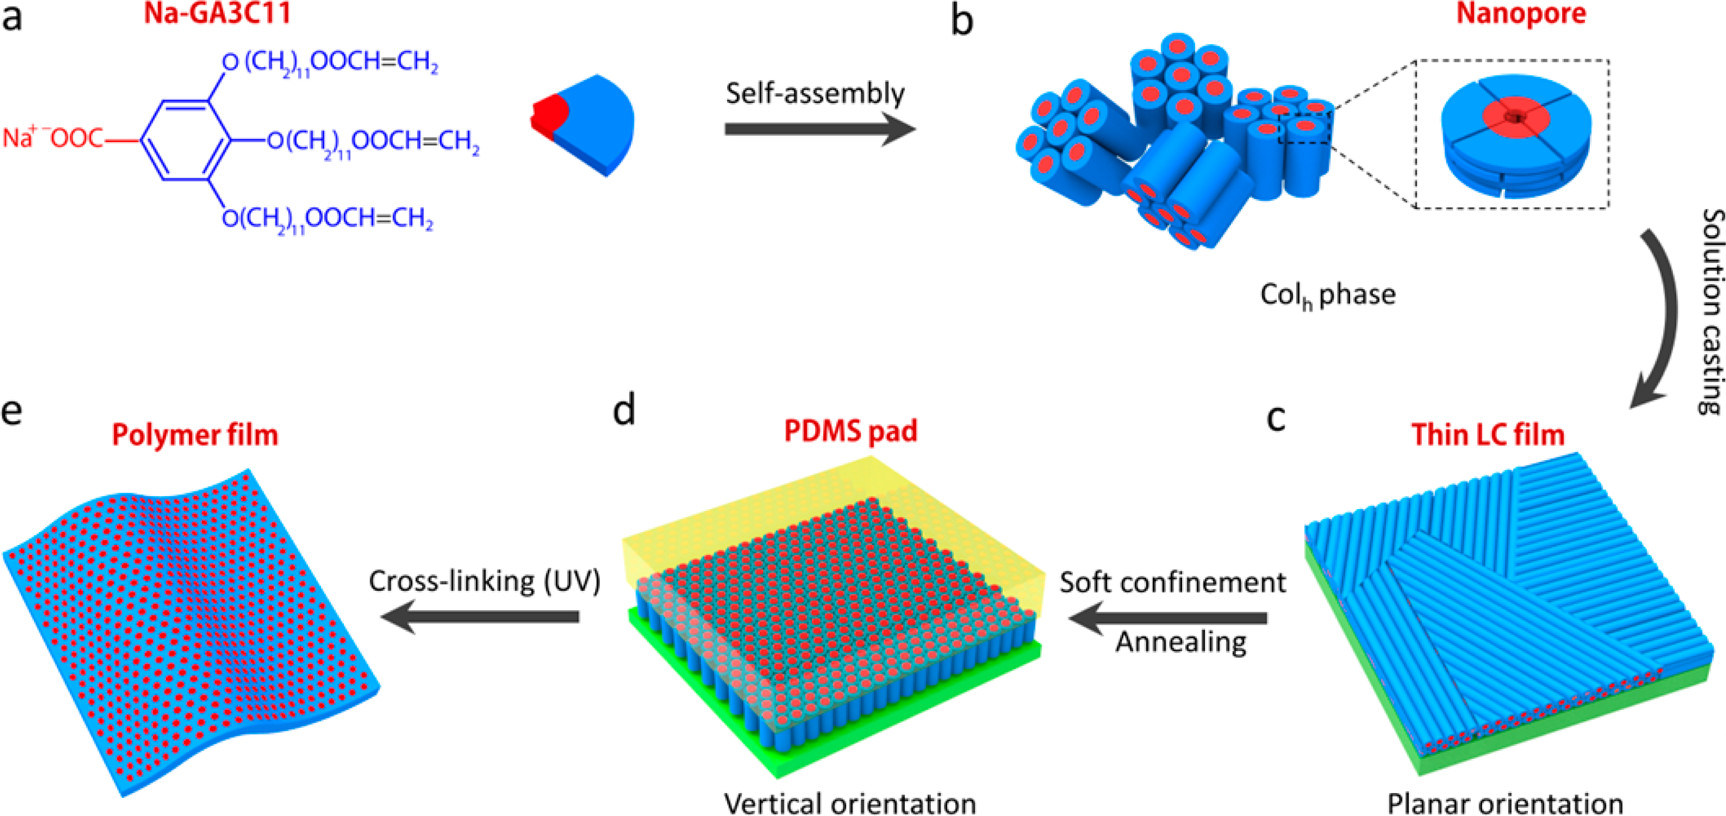
\includegraphics[width=\linewidth]{soft_confinement.png} \caption{The wedge
  %	  shaped liquid crystal monomer (a) self assembles into mesophases with
%		  hexagonally packed pores (b). The pores are made of stacked monomer disks. A
%		  sub-micron-thick film is created by casting a dilute solution of Na-GA3C11/THF
%		  solution onto a silicon substrate and and allowing the solvent to evaporate.
%		  The thin film contains nanoporous columns which lie parallel to the film plane.
%		  (d) When a soft PDMS pad is imposed to the thin film, with subsequent thermal
%		  annealing, the columns align perpendicular to the film plane. (e)
%		  Photo-cross-linking of the aligned film creates a mechanically stable thin film
%		  with vertically aligned nanopores}~\label{fig:soft} \end{figure}

  %BJC: Made my own version of the above, leaving out alignment details since it'

  %BJC: TODO: Scalable vector graphic for monomer structure, make bigger. Convert .svg to .eps
  %           Thicken slabs
  %           Make pore region on slab (blue) bigger
  %           Bump up atom sizes in atomistic render
  \begin{figure}
	\centering
	\begin{subfigure}{.3\textwidth}
		\centering
		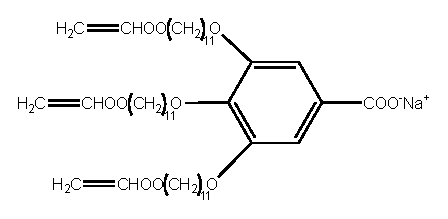
\includegraphics[width=\textwidth]{NaGA3C11.eps}
		\caption{}~\label{fig:monomer}
	\end{subfigure}
	\begin{subfigure}{.3\textwidth}
		\centering
		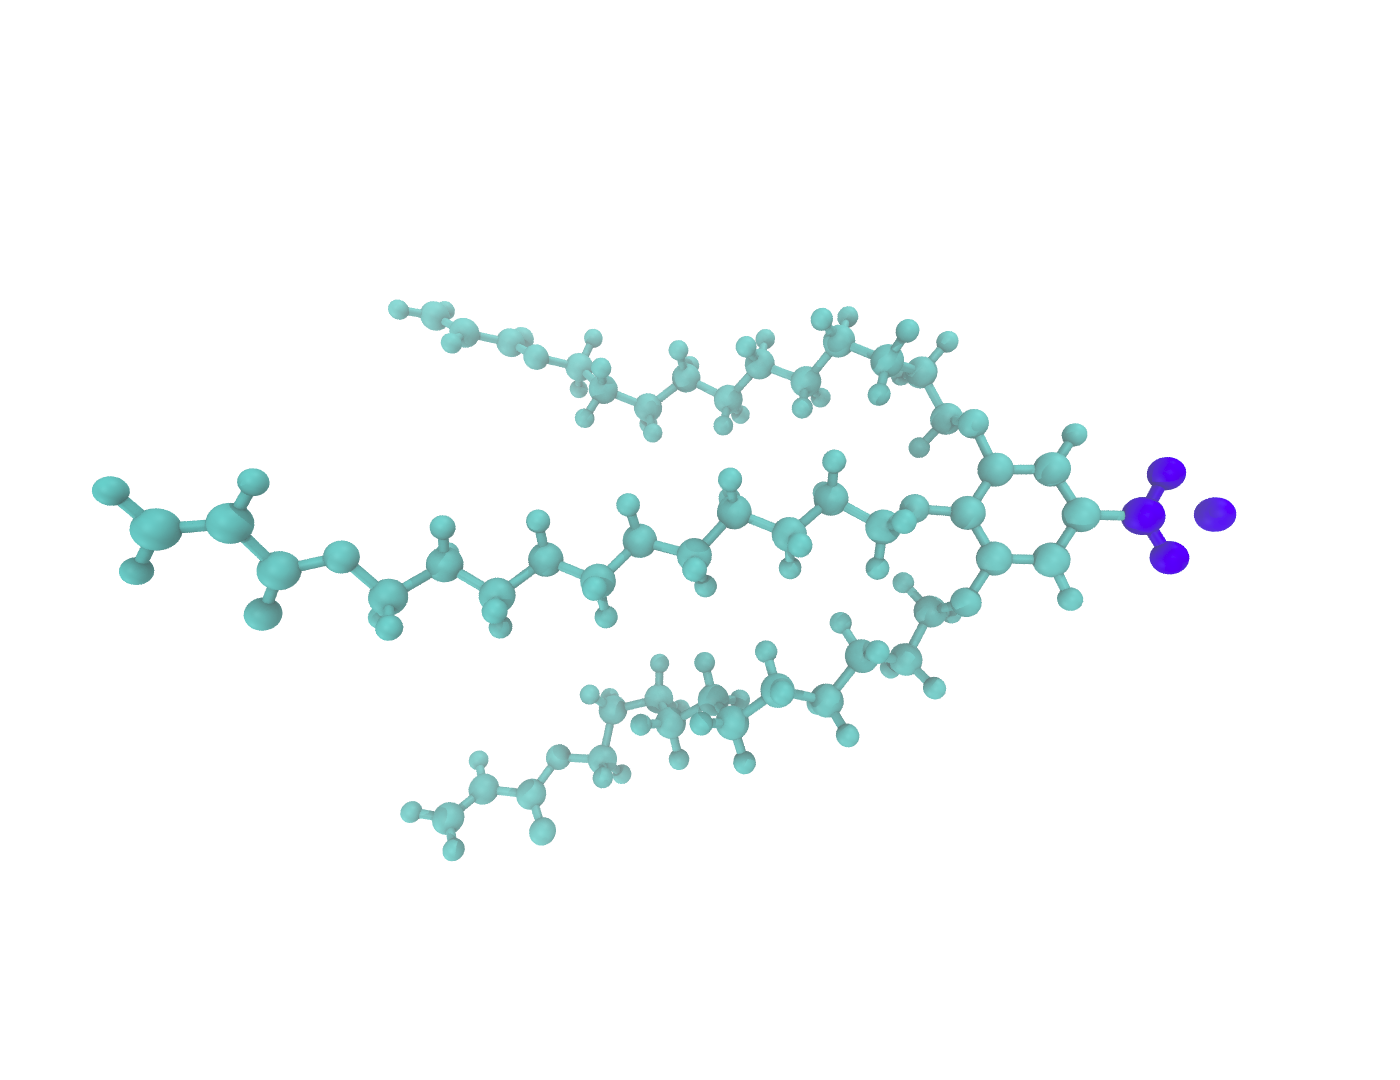
\includegraphics[width=\textwidth]{monomer_twocolor.png}
		\caption{}~\label{fig:atomistic_monomer}
	\end{subfigure}
	\begin{subfigure}{0.3\linewidth}
		\centering
		
\includegraphics[width=\textwidth]{wedge_thick.png}
		\caption{}~\label{fig:wedge}
	\end{subfigure}
		\begin{subfigure}{0.4\linewidth}
		\centering
		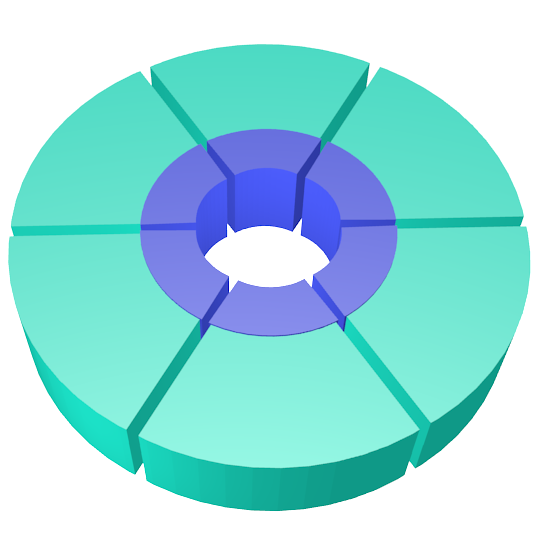
\includegraphics[width=\textwidth]{layer_thick.png}
		\caption{}~\label{fig:wedge_layer}
	\end{subfigure}
	\begin{subfigure}{0.4\linewidth}
		\centering
		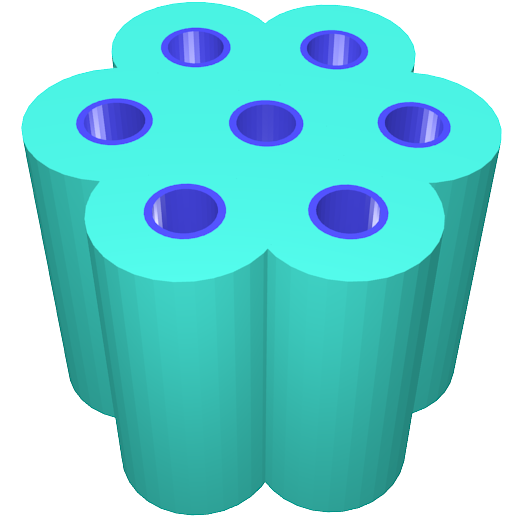
\includegraphics[width=\textwidth]{hexagonal_packing.png}
		\caption{}~\label{fig:hex_packing_simple}
	\end{subfigure}
	\caption{The LLC monomer Na-GA3C11 (a) rendered atomistically (b)
	exhibits wedge-like character (c). Monomer wedges assemble into disks (d) with
	hydrophilic head groups (blue) facing towards the disk center. The disks
	assemble into hexagonally packed columnar mesophases (e).}~\label{fig:assembly}
  \end{figure}

  Our current understanding of LLC systems is not rich enough to be able to
  precisely design membranes for specific separations. Over the past 20 years,
  H\textsubscript{II}-phase LLC polymer membrane studies have been limited
  primarily to Na-GA3C11 with some characterization done after minor structural
  modifications. Resel et al.~varied the length of the monomer tails and the
  counterion used and observed its affect on pore spacing
  \cite{resel_structural_2000}. In a later study of rejection performance, it
  was shown that membranes formed by cross-linked Na-GA3C11 in the
  H\textsubscript{II} phase cannot separate solutes less than 1.2 nm in
  diameter because the pores are too large \cite{zhou_supported_2005}. We do not
  yet understand how to controllably reduce the effective pore size or how to
  tune the chemical environment in the nanopores of this or related materials for
  effective water desalination and small organic molecule separations. The only
  source of predictive modeling for LLC systems have been macroscopic models that
  likely do not adequately describe transport at these length scales
  \cite{hatakeyama_water_2011}. It will be challenging to efficiently narrow down
  the large design space in a laboratory setting without a robust model.

  In this study, we build a significantly more realistic atomistic model of LLC
  membranes than, to our knowledge, has ever previously been done, and explore
  what new structural information can be gained and what structure hypotheses are
  supported by this model. We validate the model using as much experimental
  information as possible. We are most interested in reproducing the conclusions
  about structure drawn from small angle X-ray scattering (SAXS)
  and wide angle X-ray scattering (WAXS) experiments as well as in matching ionic
  conductivity measurements \cite{feng_thin_2016}.

  A molecular-level understanding of LLC polymer membrane structure, enabled by
  molecular dynamics simulations, can provide guidelines to reduce the large
  chemical space available to design monomers for creation of separation-specific
  membranes. A good molecular model should incorporate a detailed picture of the
  nanoscopic pore structure which will be crucial to understanding the role of
  monomer structure in solute transport and membrane design. Models resulting
  from molecular dynamics simulations will provide the required level of detail
  (Fig. \ref{fig:detail}), assuming the force fields are sufficiently accurate.
  With such an atomistic model, we can directly observe molecular-level solute
  transport and suggest governing mechanisms. We can observe how the choice of
  head group may influence pore size for size exclusion driven separations. We
  can interchange counterions which may influence both the pore size and the
  strength of the Donnan potential which affects the degree to which the membrane
  can exclude charged species. 

  \begin{figure}
  \centering
	\begin{subfigure}{0.45\linewidth}
		\centering
		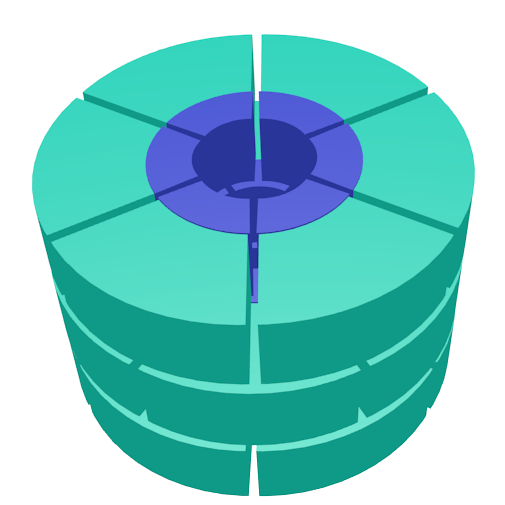
\includegraphics[width=\textwidth]{cartoon_pore.png}
		\caption{}~\label{fig:undetailed_pore}
	\end{subfigure}
	\begin{subfigure}{0.45\linewidth}
		\centering
		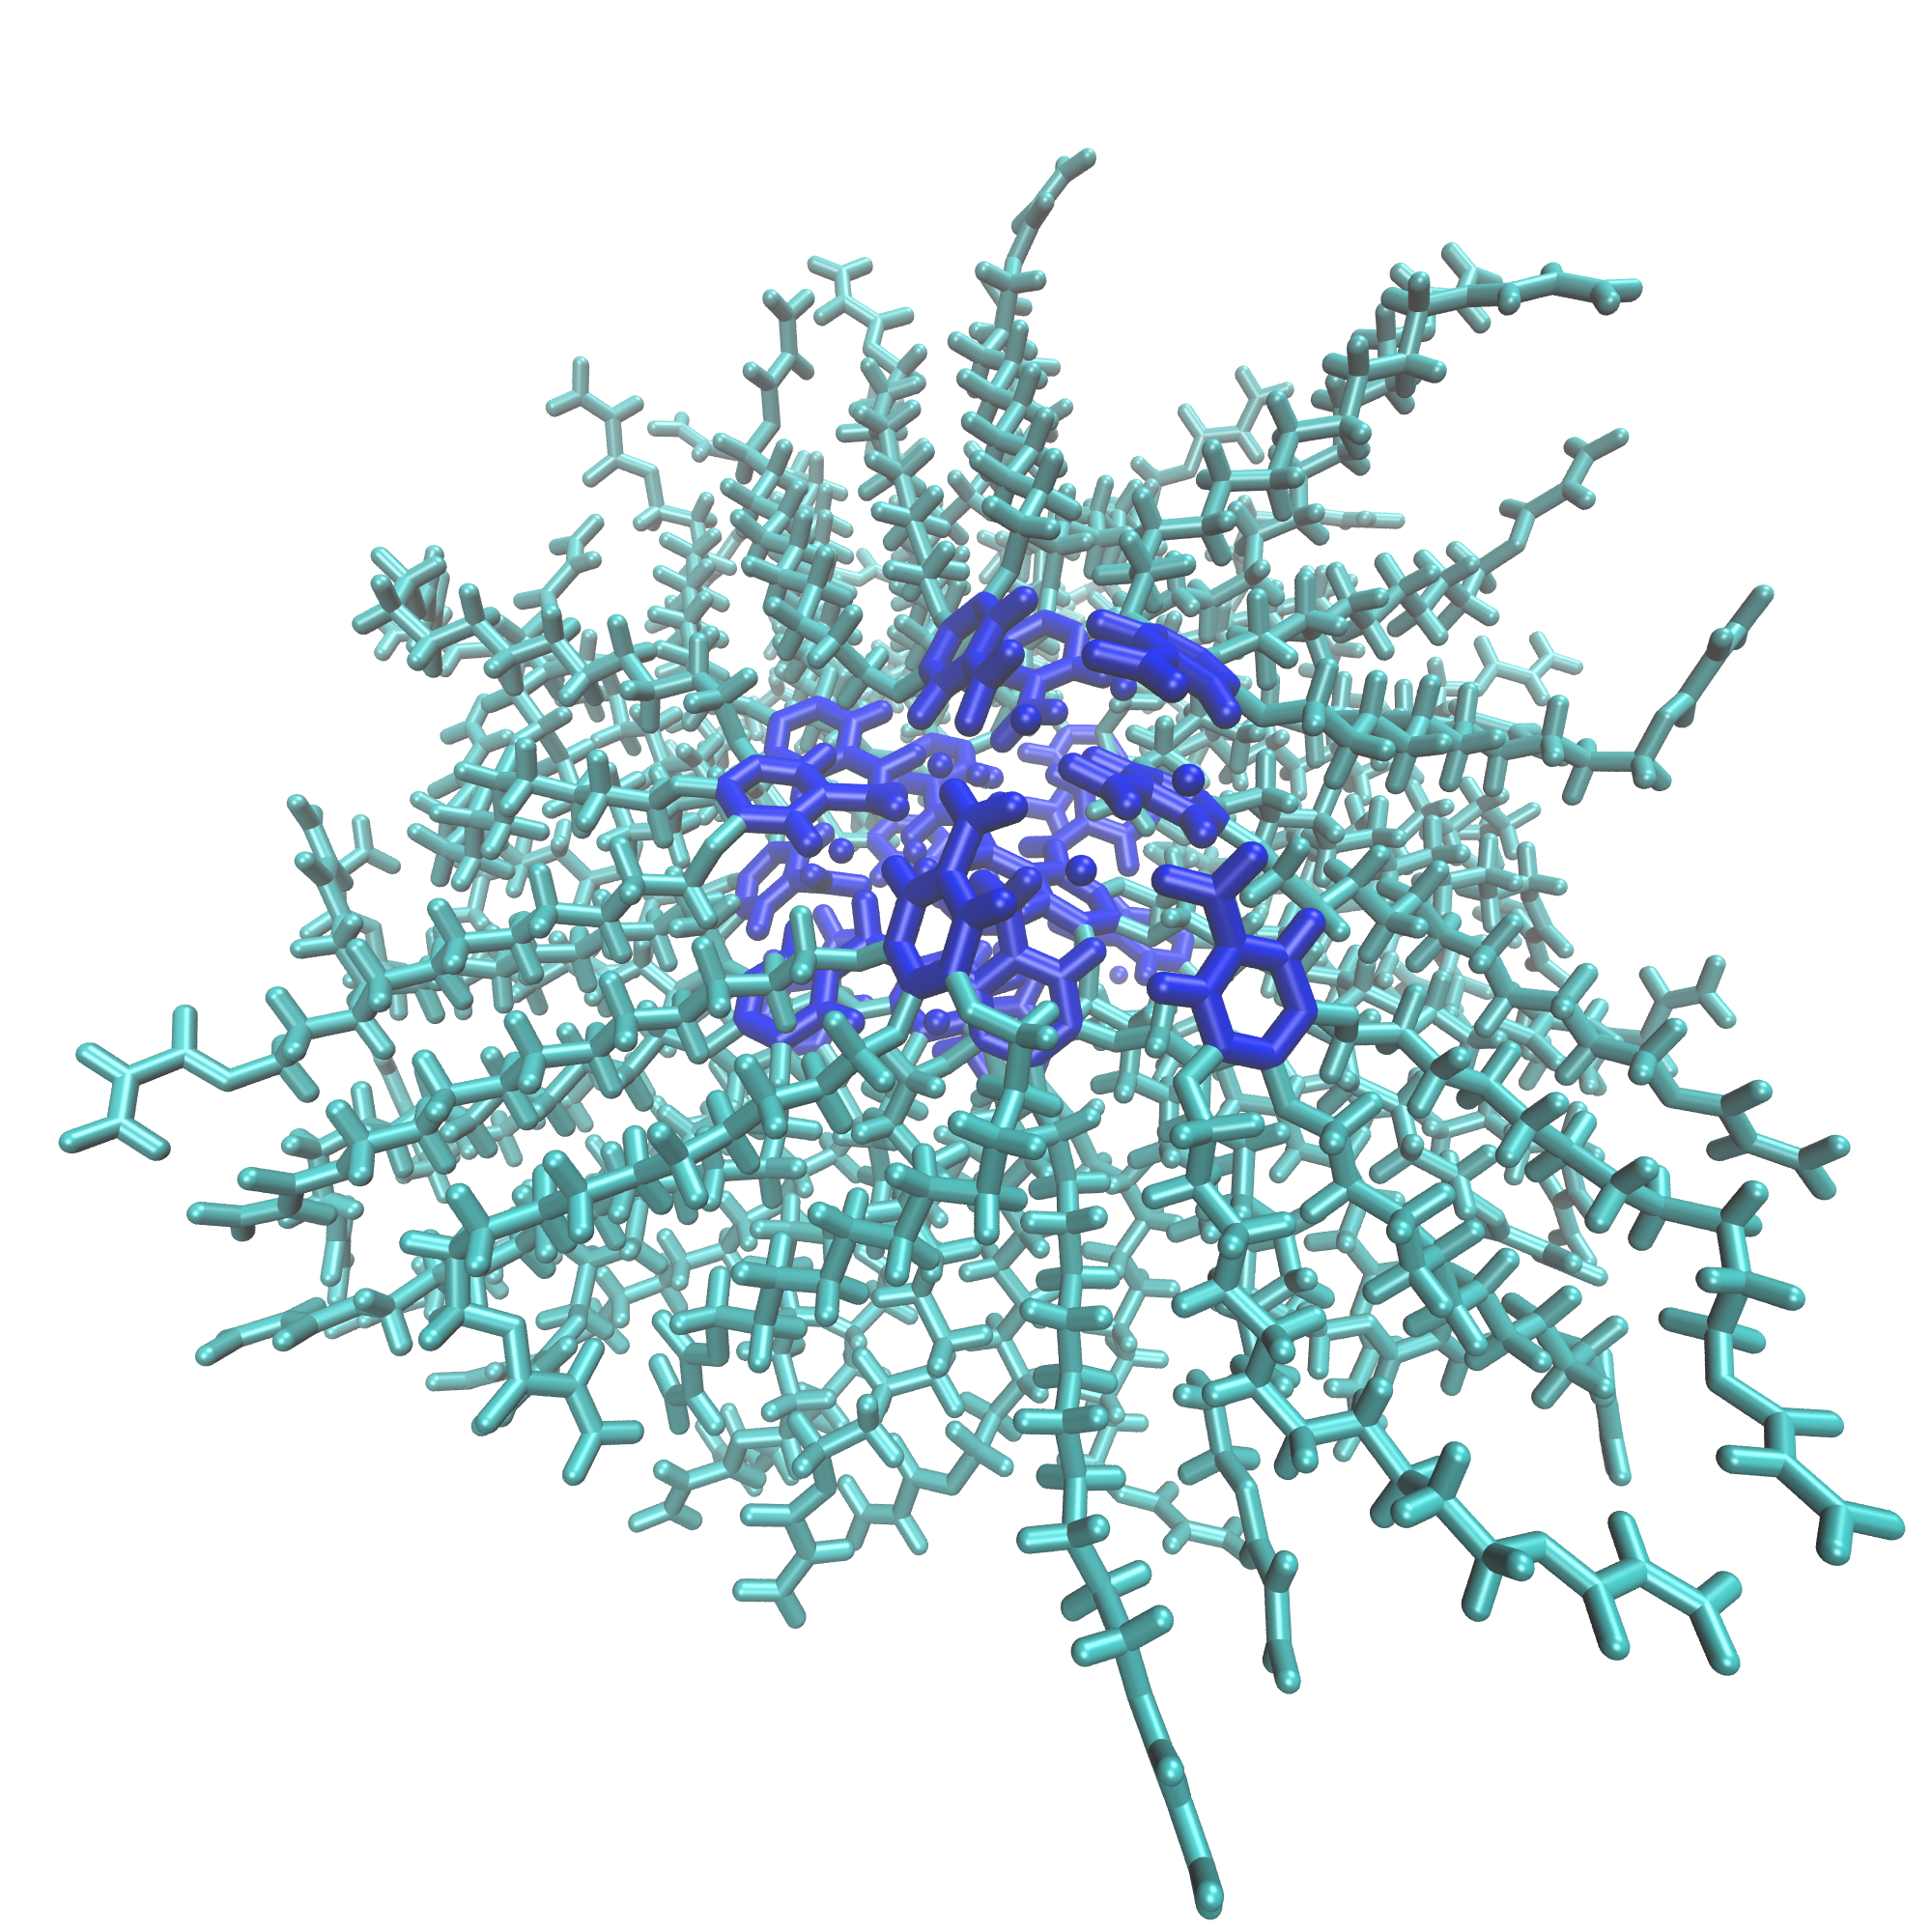
\includegraphics[width=\textwidth]{detailed_pore.png}
		\caption{}~\label{fig:detailed_pore}
	\end{subfigure}
  \caption{We can only speculate about solute behavior inside the membrane
	  pores based on our previous picture of the pore structure (a). We will use a
	  detailed molecular model in order to appropriately model the pore's complex
	  architecture which is crucial to understanding the mechanism of solute
	  transport (b). The head group region is colored blue
	  and the tail region is colored cyan in both representations.}~\label{fig:detail}
  \end{figure}
 
  %BJC: I think the first sentence of the following paragraph is
  %necessary to put somewhere, but maybe not in this spot exactly
  In order to appropriately model transport in these ordered, nanoporous
  organic systems, we must first gain a thorough understanding of the nanoscopic
  structure of LLC polymer membranes. Our approach to constructing a general
  model will follow the development of a model of the assembly formed by
  Na-GA3C11 since it has sufficient experimental characterization. We have also
  narrowed our scope to the development of a model of the Col\textsubscript{h}
  phase membrane. Compared to the H\textsubscript{II} phase, the
  Col\textsubscript{h} phase is a simpler starting point, due to the absence of
  water, and has detailed experimental wide-angle X-ray scattering (WAXS)
  patterns useful for reconstructing structural data. The two phases appear to
  share similar structural characteristics since the pore spacings in each system
  are in close agreement \cite{feng_thin_2016,resel_structural_2000}.

  Despite having structural data, there is still information which experiment
  cannot definitively answer. Our current level of understanding suggests that
  monomers partition into layers with head groups facing towards the center, then 
  stack on top of each other to create pores that pack together hexagonally.
  There are several key questions that we will investigate in order to
  expand this understanding:
 
  \begin{enumerate}

  \item If layers do exist, how many monomers constitute a single layer? \label{point:monomernum}
  
  A simple molecular simulation study of a similar molecule suggested that
  there are 4 monomers in each layer \cite{zhu_methacrylated_2006}. Their 
  model likely does not sufficiently model the chemical environment present
  in the real system since it only contains 16 total monomers.
%BJC3: rephrased
%  However, their estimate is based on a simulated system that contains 16 total
%  monomers which likely does not sufficiently model the chemical environment
%  present in the real system
  A separate calculation based on the estimated volume of the liquid crystal
  monomers proposes that each layer consists of seven monomers
  \cite{resel_structural_2000}. Our best chance to answer this question is by
  using a molecular model orders of magnitude larger than any other reported
  atomistic liquid crystal membrane simulation, as we present here. We will
  directly change the layer composition and note its effect on membrane
  structure.

  \item Does our model support the existence of layers and if so, how well
  defined are the layers? \label{point:layers} 

  Strong $\pi$-$\pi$ stacking interactions in the direction perpendicular to
  the membrane plane support the existence of layers experimentally. $\pi$-$\pi$
  stacking will only occur between the aromatic monomer head groups which leaves
  no description of what is happening in the monomer tail region. The tails may
  entangle isotropically while maintaing stacking order among headgroups. 

  \item How do monomers in each layer position themselves with respect to
  surrounding layers? \label{point:orientation}

  The $\pi$-$\pi$ stacking interactions may be a driving force of self-assembly
  in this system \cite{gazit_possible_2002}. Gas phase ab initio studies of
  benzene dimers have shown a clear energetic advantage for parallel displaced
  and T-shaped $\pi$-$\pi$ stacking conformations over a sandwiched
  conformation \cite{sinnokrot_estimates_2002}. Substituted benzene rings
  exhibit an even stronger $\pi$-$\pi$ stacking attraction which favors the
  parallel displaced configuration in all cases except where the substitutions
  are extremely electron withdrawing.
  \cite{waller_hybrid_2006,ringer_effect_2006} In this study, we compare
  simulated X-ray diffraction patterns to experiment in order to deduce which
  stacking configuration is most likely. 

  \item Can the system exist in other metastable states or phases that are not
  accessed during experiments? \label{point:metastable}
  
  There remains the possibility that there is more than one metastable state
  associated with a given LLC phase. Simulating a membrane atomistically
  requires many atoms which limits the timescales acessible with MD. It is
  reasonable to expect that we will generate configurations which are kinetically
  trapped in a metastable free energy basin. We must be able to identify which
  state is produced experimentally.

  %\item What constitutes a pore, and how well-defined are the pore regions? \label{point:poredefinition}
  \item What constitutes a pore, and what does the pore architecture look like? \label{point:poredefinition}

  The limited picture that experiment provides tells us that there are
  hexagonally packed, hydrophilic regions where transport is likely to occur.
  One may instinctively assume that these regions are tube-like pathways. We will
  explore the composition of the pores and the partition between the
  hydrophilic and hydrophobic regions. 

  \item Is it necessary to include any water in order to appropriately model
  the Col\textsubscript{h} phase? \label{point:water}

  While past work describes the Col\textsubscript{h} phase as dry
  ~\cite{feng_scalable_2014}, it has been suggested by experimentalists, in
  unpublished communications, that it is likely that neat monomer leaches small
  amounts of ambient water. Experimentally, achieving a hexagonal phase with a
  completely dry system has proven difficult. If neat monomer sits in ambient
  conditions, its color turns from transparent to slightly opaque and a hexagonal
  phase forms. Although we will not explore whether water is necessary for
  self-assembly, we hypothesize that the hydrogen bonding network formed by the
  water may play a role in structuring the pores and holding together the
  hexagonal phase. We can use simulated X-ray diffraction patterns to see if
  there is any meaningful structural difference between a ``dry'' and ``wet''
  system.

  \end{enumerate}
  
  %Once we have addressed all of the above questions, we must show that the 
  %developed molecular model is consistent with physical observations so that we
  %can rely on conclusions drawn about structural features characteristic of 
  %the system.
 
  We used experimental small-angle X-ray scattering (SAXS) data from
  \cite{feng_thin_2016} (Fig.~\ref{fig:SAXS}) and wide angle X-ray scattering
  (WAXS) data (Fig.~\ref{fig:WAXS}, produced as described in
  \cite{feng_scalable_2014}) for comparison to our model. We rely primarily on the 2D WAXS data
  since it encodes all structural details down to the sub-nm scale.  There are
  five major features of interest present in the 2D experimental pattern shown in
  Figure \ref{fig:WAXS}.

  \begin{enumerate} 
  
	\item The location of the first is at $q_z$ = 1.7 \angstrom$^{-1}$,
	corresponding to a real space separation of 3.7 \angstrom~. Previous
	work~\cite{feng_scalable_2014} attributes this reflection to $\pi$-$\pi$
	stacking between aromatic rings in the direction perpendicular to the membrane
	plane, or z-axis \cite{feng_scalable_2014}. For simplicity, we will refer to
	this reflection as R-$\pi$.
 
	\item A weak intensity line, located at exactly half the $q_z$ value of
	R-$\pi$ ($q_z$ = 0.85 \angstrom$^{-1}$), corresponds to a real space periodic
	spacing of 7.4 \angstrom~. This reflection has been interpreted as
	2\textsubscript{1} helical ordering of aromatic rings along the z axis
	\cite{feng_scalable_2014}, meaning that if one traces the positions of the
	aromatic rings with a helical curve, then for each full turn in the helix, one
	will encounter two aromatic rings. For this reason we will refer to reflection
	as R-helix. 

	\item A low intensity ring located at r = 1.4 \angstrom$^{-1}$ marks
	the third major reflection of interest. The real space separation corresponds
	to 4.5 \angstrom~ which is characteristic of the average spacing between packed
	alkane chains \cite{mcintosh_organization_1980}. We will call this reflection
	R-alkanes.

	\item Within R-alkanes, are four spots of higher relative intensity.
	Accordingly, we name these reflection R-spots. The location of all spots is $\sim 37$
	degrees from the $q_z$ axis in their respective quadrants. In many liquid
	crystal systems one can explain the spots by the tilt angle of the alkane chains
	with respect to the membrane plane \cite{govind_simple_2001}.
 
	\item The final feature corresponds to the spacing and symmetry of the
	d\textsubscript{100} plane. This plane is geometrically related the distance
	between pores. The feature, which we named R-pores, is characterized by dots
	along the equatorial axis defined when $q_z$ = 0. The spacing between dots is
	indicative of the hexagonal symmetry of the packed pores. We observe the same
	information with higher resolution using SAXS (Fig.~\ref{fig:SAXS}). 

  \end{enumerate}

  %BJC: TODO: update colorbar
  \begin{figure}
        \centering
        \begin{subfigure}[t]{0.43\linewidth}
                \centering
                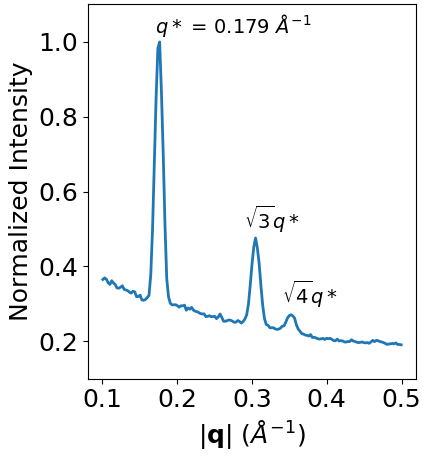
\includegraphics[width=\linewidth]{SAXS.png}
                \caption{}\label{fig:SAXS}
        \end{subfigure}
        \begin{subfigure}[t]{0.47\linewidth}
                \centering
                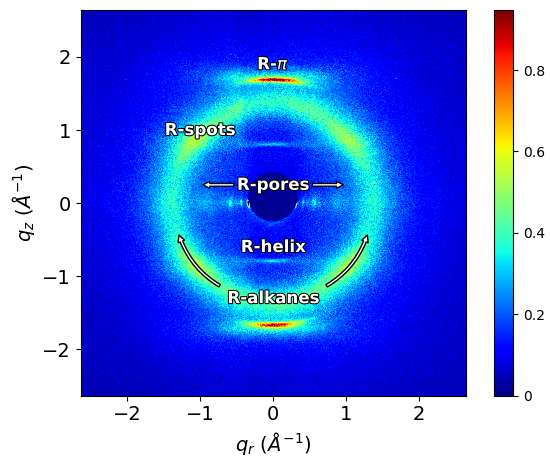
\includegraphics[width=\linewidth]{WAXS_annotated_words.png} 
                \caption{}\label{fig:WAXS}
        \end{subfigure}
%BJC: What do you think of the labels now? I tried to make it more clear what each label refers
% to graphically. I can't decide if it's too cluttered. An alternative is to number them as  
% I had them before, and then define them in a little box inset to the figure
	\caption{(a) (Reproduced from \cite{feng_thin_2016}) The repeat spacing
		in the 1D small angle X-ray scattering pattern is characteristic of hexagonal
		packing. The leading peak, q*, represents the distance between the
		d\textsubscript{100} planes. Using this distance, we know that the distance
		between pore centers is 4.12 nm. (b) 2D WAXS gives
		details about repeating features on the order of angstroms. Experimentalists
		have explained each of the 5 major reflections present as follows: (R-$\pi$) Aromatic
		head groups $\pi-\pi$ stack 3.7 \AA~apart. (R-helix) Monomers arrange vertically in
		a 2\textsubscript{1} helix. (R-alkanes) Alkane chain tails pack 4.5 \AA~apart. (R-spots)
		Monomer tails are tilted with respect to the membrane plane. (V) As derived from
		SAXS, the pores are spaced 4.12 nm apart and pack hexagonally}
	\label{fig:SWAXS}
 \end{figure}

  \section{Methods}
 
  \subsection{Monomer Parameterization}

  We parameterized the liquid crystal monomers using the Generalized AMBER
  Force Field \cite{wang_development_2004} with the Antechamber package
  \cite{wang_automatic_2006} provided with AmberTools16
  \cite{case_ambertools16_2016}. We assigned atomic charges using the am1bccsym
  method of \texttt{molcharge} shipped with QUACPAC from Openeye Scientific
  Software. We ran all molecular dynamics simulations using Gromacs 2016
  \cite{bekker_gromacs:_1993,berendsen_gromacs:_1995,van_der_spoel_gromacs:_2005,hess_gromacs_2008}.

  We generated an ensemble of characteristic, low-energy vacuum monomer
  configurations by applying a simulated annealing process to a
  parameterized monomer. We cooled monomers from 1000K to 50K over 10
  nanoseconds. We randomly pulled a low energy configuration from the
  trajectory then reassigned charges using \texttt{molcharge}. Using the new
  charges, we annealed the monomer system again and pulled a random monomer
  configuration from the trajectory which we used for full system
  construction (Figure~\ref{fig:python}a). See supplemental information for
  further detail.

% Note: we should put scripts and starting configurations (not all that were
% done but the important ones) in a public repository by the time of
% submission. 
%MRS4: I would give a ``plain text'' version of the script in supplementary. BJC: referring to parameterization script
%MRS4: somewhere would need to specify things like time step tau_t, tau_p, etc., so that people could in theory replicate 

  \subsection{Unit Cell Preparation}

%MRS4: check grammar additions in this paragraph.
  The timescale for self-assembly of monomers into the hexagonal phase is
  unknown and likely outside of a reasonable length for an atomistic simulation,
  calling for a more efficient way to build the system. Previous work has shown
  a coarse-grained model self assemble into the H\textsubscript{II} phase
  configuration in $\sim$1000 ns \cite{mondal_self-assembly_2013}.  We
  attempted atomistic self-assembly by packing monomers into a box using Packmol
  \cite{martinez_packmol:_2009}.  Simulations of greater than 100 ns show no
  indicators of progress towards an ordered system. To bypass the slow
  self-assembly process, we use Python scripts to assemble monomers into a
  structure close to one of a number of hypothesized equilibrium configurations
  (Figure~\ref{fig:python}).

  %BJC: TODO: reproduce figure in latex (or gimp?) with higher resolution arrows
  \begin{figure}
	\centering
	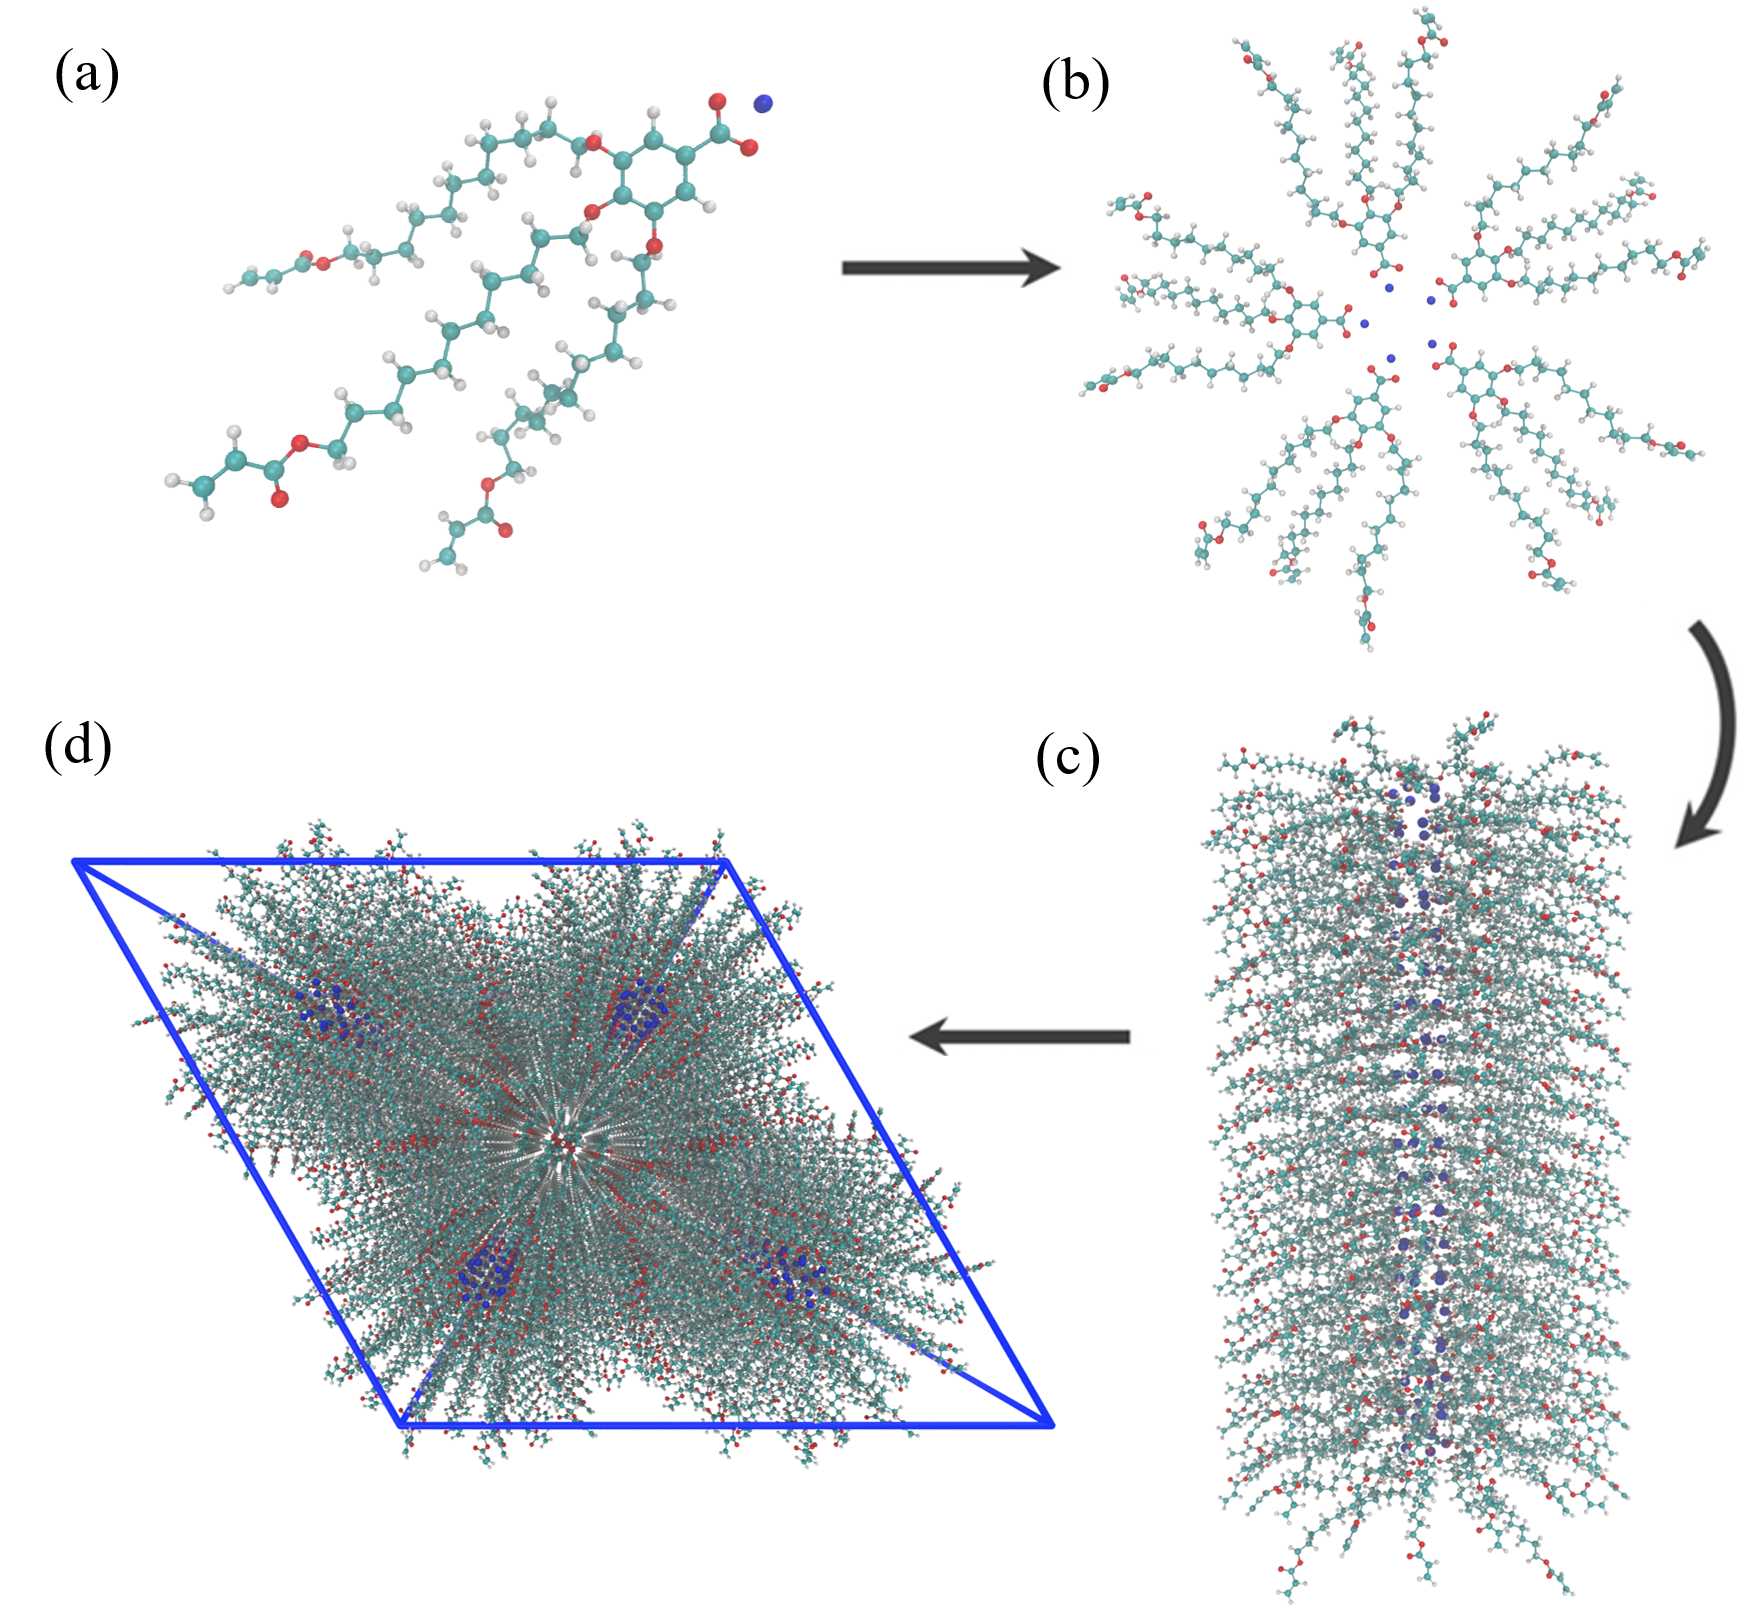
\includegraphics[width=0.75\linewidth]{build.PNG} %BJC: put an xyz axis with the unit cell
	\caption{(a) We parameterized a single monomer and annealed it to produce a low energy
		configuration. (b) A python script rotates and assembles monomers into layers with 
		hydrophilic centers. (c) We chose to stack twenty layers on top of each other to create
		pores. (d) The pores are duplicated and placed into a monoclinic unit cell}\label{fig:python}
  \end{figure}
  
  A typical simulation volume contains four pores in a monoclinic unit cell,
  the smallest unit cell that maintains hexagonal symmetry when extended
  periodically. Each pore is made of twenty stacked monomer layers with periodic
  continuity along the pore axis, avoiding any edge effects and creating an
  infinite length pore ideal for studying transport. We prefer a small number of layers
  in order to reduce computational cost and to allow us to look at
  longer timescales. Ultimately, we chose to build a system with 20 monomer
  layers in each pore in order to obtain sufficient resolution when simulating
  X-ray diffraction patterns. %This point will be explained in more detail later.
%MRS3: isn't there some observations you need at least 10?  
%BJC2: When I first set up the system, there was a gap and a small number of layers 
% appeared to cause the phase to disassociate. However, I can get a pretty small
% number of layers in the infinite pore system, but the diffraction is low resolution.

\subsection{Monomer Placement} 

  When constructing an initial configuration, there are a number of variables
  which require careful consideration while placing monomers. The equilibrium
  configuration is sensitive to some while insensitive to others. The starting
  pore radius, defined as the distance of a chosen head group carbon from the
  pore's central axis, does not influence the equilibrium structure if one choses
  a reasonable value (See Supplemental Information). The pore radius is chosen to
  be 0.5 nm in our initial configurations. The initial distance between pores
  also has little effect on the the equilibrated structure (See supplemental
  information). However, one should not start them too close or there will be
  high energy repulsions during early equilibration. We chose an initial pore
  spacing of 4.5 nm, $\sim$10\% larger than the experimental value of 4.12 nm.
  The distance between layers, the rotation of the layers with respect to
  adjacent layers, and the number of monomers per layer do influence the
  equilibrium structure and require further justification for their choices.  We
  rely on experimental data to inform them. 

  We chose the layer spacing for the initial configuration based on R-$\pi$ and
  then allowed the system to readjust during equilibration. Each monomer was
  rotated so the plane of the aromatic head groups would be coplanar with the xy
  plane. We explored three different initial layer spacings. The first is exactly
  equal to R-$\pi$ with layers placed so aromatic rings stack 3.7 \AA~apart in
  the z-direction. We explore a second system with an initial layer spacing of 5
  \AA. We briefly explored a third system with an initial layer spacing of 10
  \AA. If we initially space layers too far apart, they will collapse on each
  other while simultaneously slipping in between layers of adjacent pores, which
  leads to an artificially thick membrane with pores spaced closely together.
  Further details of simulations with layer stacked 10 \AA apart are in the supplemental
  information.

  We chose the relative interlayer orientation based on clues from diffraction
  data as well as the various known stacking modes of benzene and substituted
  benzene rings: sandwiched, parallel-displaced and T-shaped
  \cite{sinnokrot_estimates_2002} (Fig. \ref{fig:sandwiched} and
  \ref{fig:pd,fig:tshaped}).  We ruled out the T-shaped configuration because its
  $\sim$5 \angstrom~ equilibrium stacking distance
  \cite{sinnokrot_estimates_2002} is inconsistent with R-$\pi$. It is also
  infeasible for the monomers to orient in the T-shaped conformation because of
  the bulky tail groups. We will explore the system's preference towards the
  sandwiched vs. parallel displaced stacking modes in some detail. Both have
  reported stacking distances near the R-$\pi$ value of 3.7 \angstrom. Headgroups
  in our sandwiched initial configuration stack directly on top of each other
  while headgroups in the parallel displaced initial configuration stack
  with an offset of $180/nmon$ degrees where $nmon$ equals the number of monomers
  per layer.

  The number of monomers in each layer is unknown, as stated in
  (\ref{point:monomernum}). We tested configurations constructed with a varied
  number of monomers per layer. We built systems in the offset and parallel
  displaced configurations with 4, 5, 6, 7 and 8 monomers per layer.

  \subsection{Equilibration}

  We developed equilibration schemes to create dry and wet configurations. Both
  schemes start with an initial configuration generated according to the previous
  guidelines. To create a dry configuration, we fix monomer head groups in the
  sandwiched or parallel-displaced configuration using position restraints with a
  force constant of 10$^6$ kJ mol$^{-1}$ nm$^{-2}$. We run a 50 ps simulation in
  the NVT ensemble which allows the monomer tails to settle without disrupting
  the ordering of the head groups. Doing so also mitigates system dependence on
  initial monomer configuration. Every 50 ps, we reduce the force constants by
  the square root of its previous value. Once the force constant is below 10 KJ
  mol$^{-1}$ nm$^{-2}$, we reduce the restraints in a sequence with values of
  8, 3, 2, 1, and 0 KJ mol$^{-1}$ nm$^{-2}$ respectively. We allow the resulting
  unrestrained structure to equilibrate for 5 ns in the NPT ensemble
  with pressure controlled by the berendsen barostat. Next, we run long NPT
  equilibration simulations for at least 400 ns using the Parrinello-Rahman
  barostat with a time constant of 10 ps.

  In order to create a wet system, we solvated an initial configuration with
  water using \texttt{gmx solvate}. We remove all water molecules placed outside
  the pore region. Then we randomly remove water molecules inside the pore region
  until the pores reach the desired concentration of water. The remainder of the
  equilibration follows the same procedure as the dry system. 

  \subsection{Cross-linking}
  
  In order to fully match synthetic procedures, we created a cross-linking
  algorithm that one can apply to equilibrated structures. The purpose of
  cross-linking is to maintain macroscopic alignment of the crystalline domains,
  ensuring aligned, hexagonally packed pores. For that reason, we are not
  concerned with replicating the kinetics of the reaction, but instead emphasize
  the consistency of the final structure with experimental structural data. 

  We developed the algorithm based on the known reaction mechanism.
  Cross-linking of this system is a free radical polymerization (FRP) taking
  place between terminal vinyl groups present on each of the three monomer tails.
  FRPs require an initiator which bonds to the system, meaning new atoms are
  introduced into the system. For simplicity, we simulated the initiator as
  hydrogen and made it present in the simulation by including them as dummy atoms
  in all possible locations where an addition could occur. We carry out the
  cross-linking procedure iteratively. During each iteration, the algoritm
  selects eligible bonding carbon atoms based on a distance cut-off. The topology
  is updated with new bonds and dummy hydrogen atoms are changed to appropriate
  hydrogen types.  Head-to-tail addition was the only propagation mode considered
  due to its dominance in the real system \cite{young_introduction_2011}. We did
  not consider direction of attack because the resultant mixture is racemic.

  Our implementation requires long simulation times to achieve high cross-link 
  densities. A typical cross-linking procedure can take up to 24 hours. In
  order to collect equilibrated data, further NPT simulation is necessary. We
  typically run a cross-linked system for an additional 100 ns to allow the system
  to readjust. For those reasons we did not cross-link all systems tested, but only
  the most promising structure. We show that cross-linking does not significantly
  change any of our drawn conclusions in Section 3.6.

  \subsection{Equilibrium Calculations}

  Using equilibrated structures, we carry out various calculations to
  characterize the system. We define the point at which a system is equilibrated
  based on when the distance between pores stops changing.  We determined when
  the distances stopped changing by applying the statistical test,
  \texttt{pymbar.timeseries.detectEquilibration}, to the time series
  \cite{chodera_simple_2016,shirts_statistically_2008}. Simulations of 400 ns
  give at least 50 ns of equilibrated simulation trajectory.

  To calculate the equilibrated pore spacing, we measured the distance between
  pore centers. We located the pore centers by averaging the coordinates of sodium
  ions in their respective pores. We generated pore spacing statistics 
  using the bootstrapping technique (See Supplemental Information).

  To quantify the degree of layering and the equilibrium distance between layers
  in our system, we calculate a spatial correlation function, $g(z)$, measured
  along the z-axis (perpendicular to the membrane plane). To calculate $g(z)$,
  we binned the z-component distances between the center of mass of each
  component and all others of the same pore over at least 50 ns of equilibrated
  trajectory and then normalized by the average number density. To extract the
  average distance between layers we applied a discrete Fourier transform to
  $g(z)$ and extracted the highest intensity frequency.

  % BJC: To be replaced by Joe's description
  {\color{red}This section replaced by Yelk/Glaser text}. 
  Simulated X-ray diffraction patterns are generated based on atomic
  coordinates in order to make a direct experimental comparison. All atomic
  coordinates were simulated as Gaussian spheres of electron density
  corresponding to each atom's atomic number. A three dimensional Fourier
  transform (FT) of the array of electron density results in a three dimensional
  structure factor which represents the unit cell in reciprocal space. We matched
  experimental 2D WAXS patterns by adjusting the initial spacing between layers
  and the orientation of the head groups with respect to adjacent layers.

  We normalized the colorbars on all diffraction patterns relative to
  R-alkanes. We believe that the alkane-alkane density, averaged over all angles,
  is the feature most likely to be replicated between experiment and simulation.
  Other features are dependent on system ordering which is likely to have some
  dependence on initial configuration. We calculated the average intensity within
  R-alkanes of the experimental pattern, $I_{avg}$. We exclude intensities
  within $\pm$ 30\degree~of the meridional axis defined by $q_r=0$ , since the simulated patterns differ
  from experiment in those regions. Specifically, in contrast to the
  experimental WAXS pattern, R-$\pi$ appearing in simulated diffraction patterns
  intersects with R-alkanes (See Fig. \ref{fig:XRDsim}). We multiplied $I_{avg}$
  by a scaling factor of 2.5. Intensities that appear in the experimental pattern
  $\geq$ 2.5$I_{avg}$ receive colorbar values of 1. We apply the same scaling
  method to the simulated patterns. We carefully chose a scaling factor of 2.5 in
  order to (1) visibly display all features in the experimental pattern and (2)
  to allow us to compare the relative intensities of features between simulated
  and experimental diffraction patterns.

  % BJC: I think this figure belongs somewhere else 
%MRS4: yeah, probably. Possibly supplemental information.
%  \begin{figure}
%	\centering
%	\begin{subfigure}[b]{0.32\textwidth}
%		\centering
%		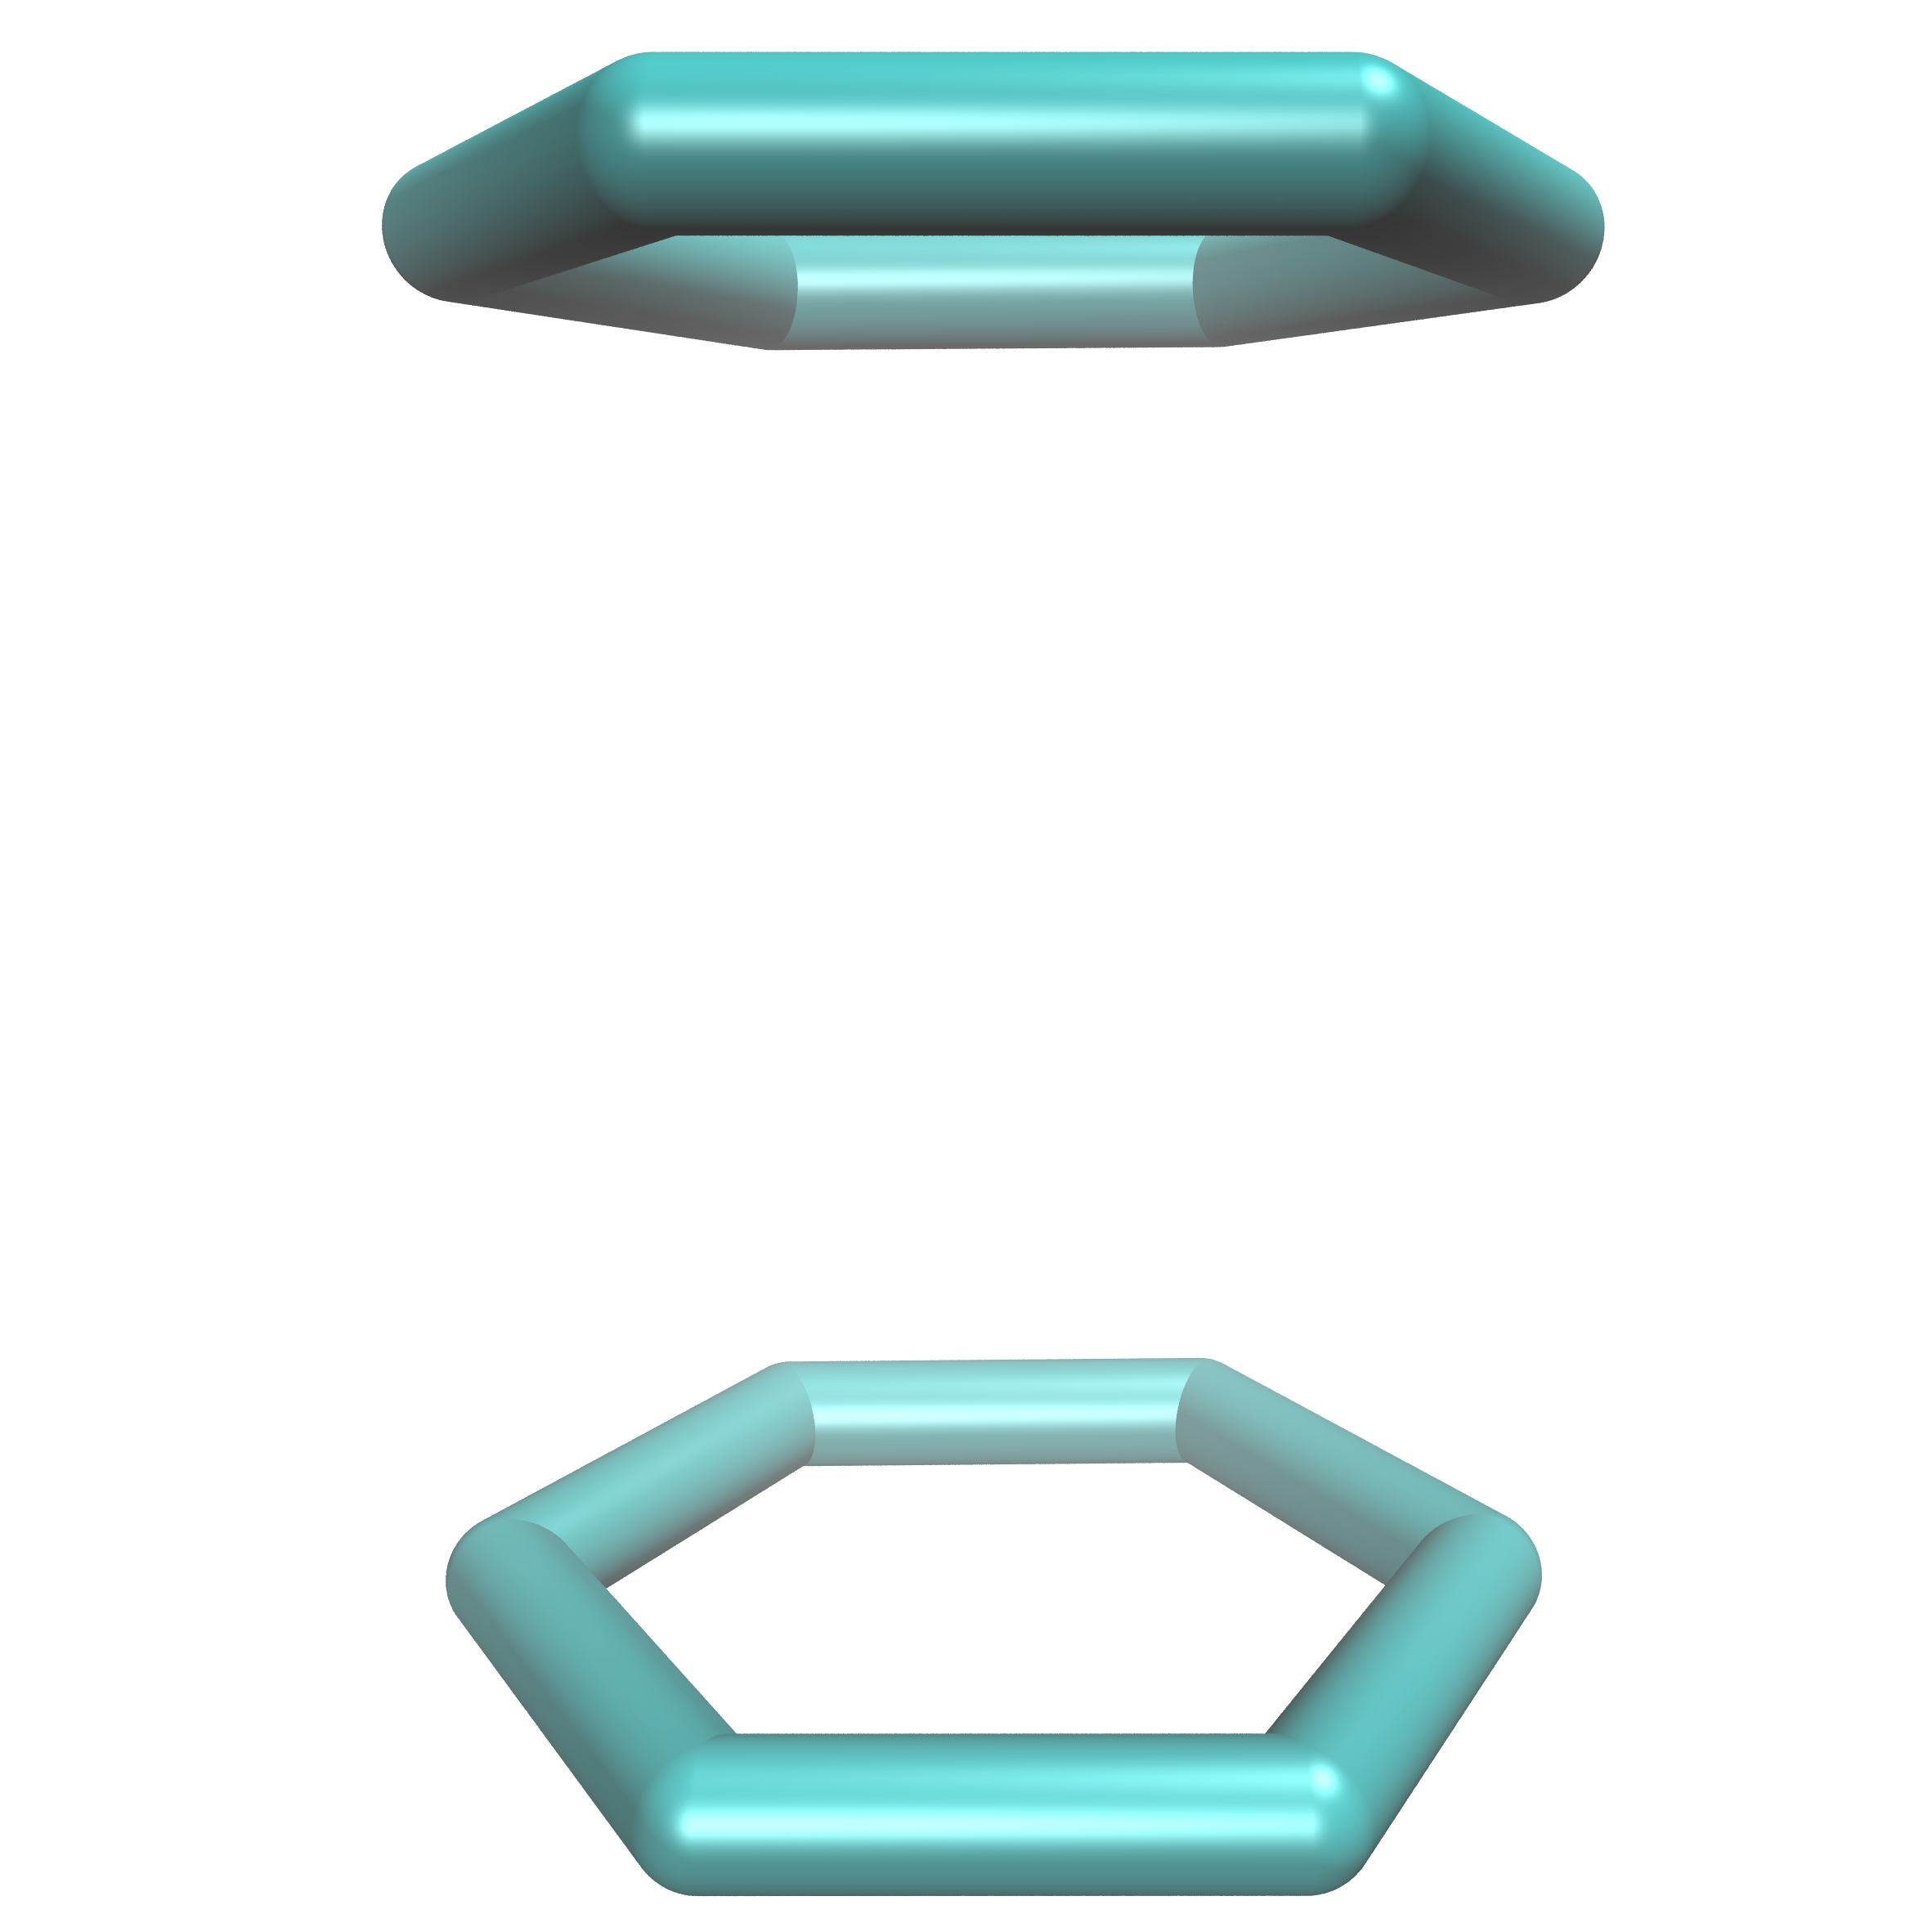
\includegraphics[width=\textwidth]{sandwiched.png}
%		\caption{}\label{fig:sandwiched}
%	\end{subfigure}
%	\begin{subfigure}[b]{0.32\textwidth}
%		\centering
%		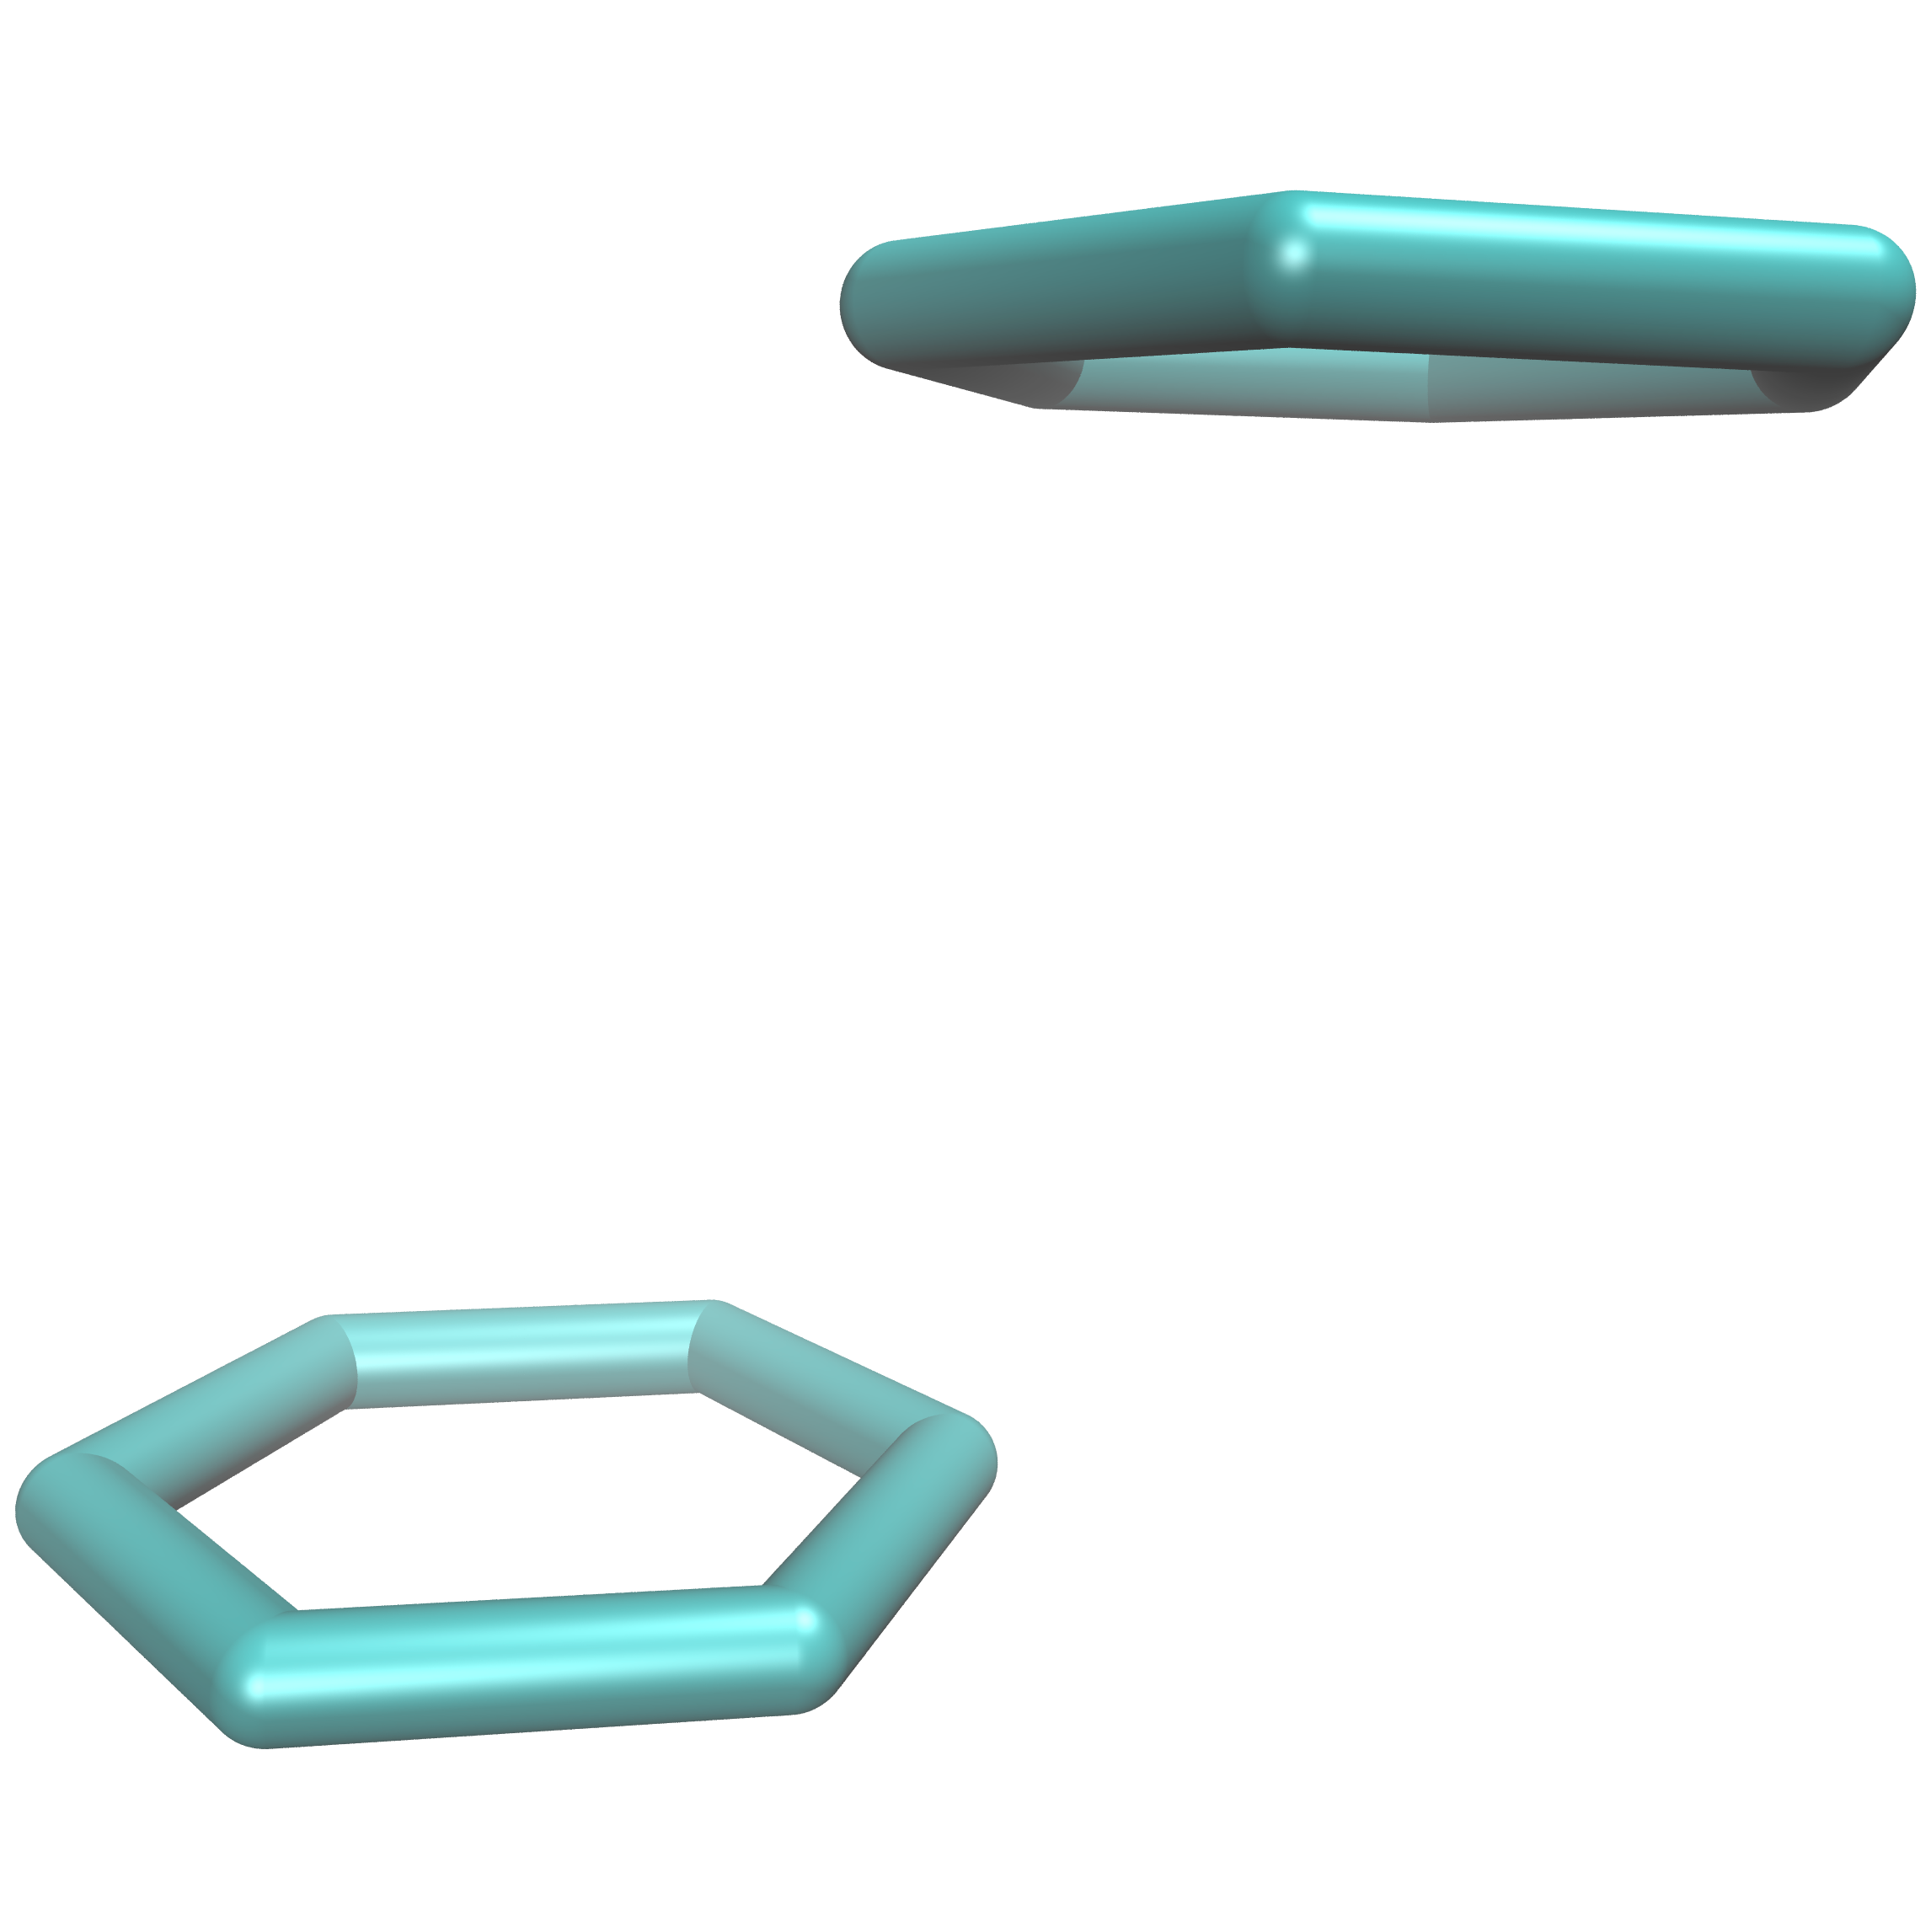
\includegraphics[width=\textwidth]{PD.png}
%		\caption{}\label{fig:pd}
%	\end{subfigure}
%	\begin{subfigure}[b]{0.32\textwidth}
%		\centering
%		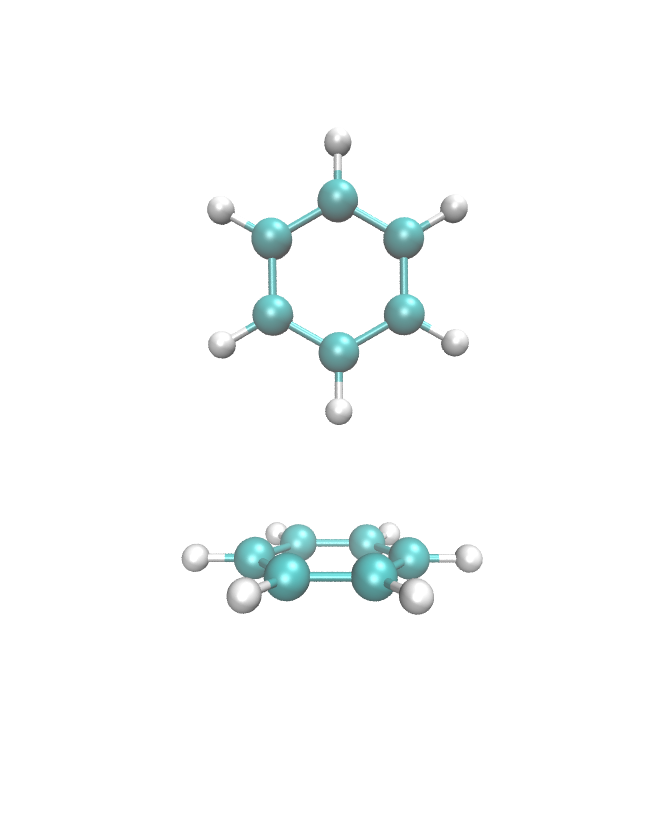
\includegraphics[width=\textwidth]{Tshaped.png}
%		\caption{}\label{fig:tshaped}
%	\end{subfigure}
%	\vskip\baselineskip
%	\begin{subfigure}[b]{0.475\textwidth}
%		\centering
%		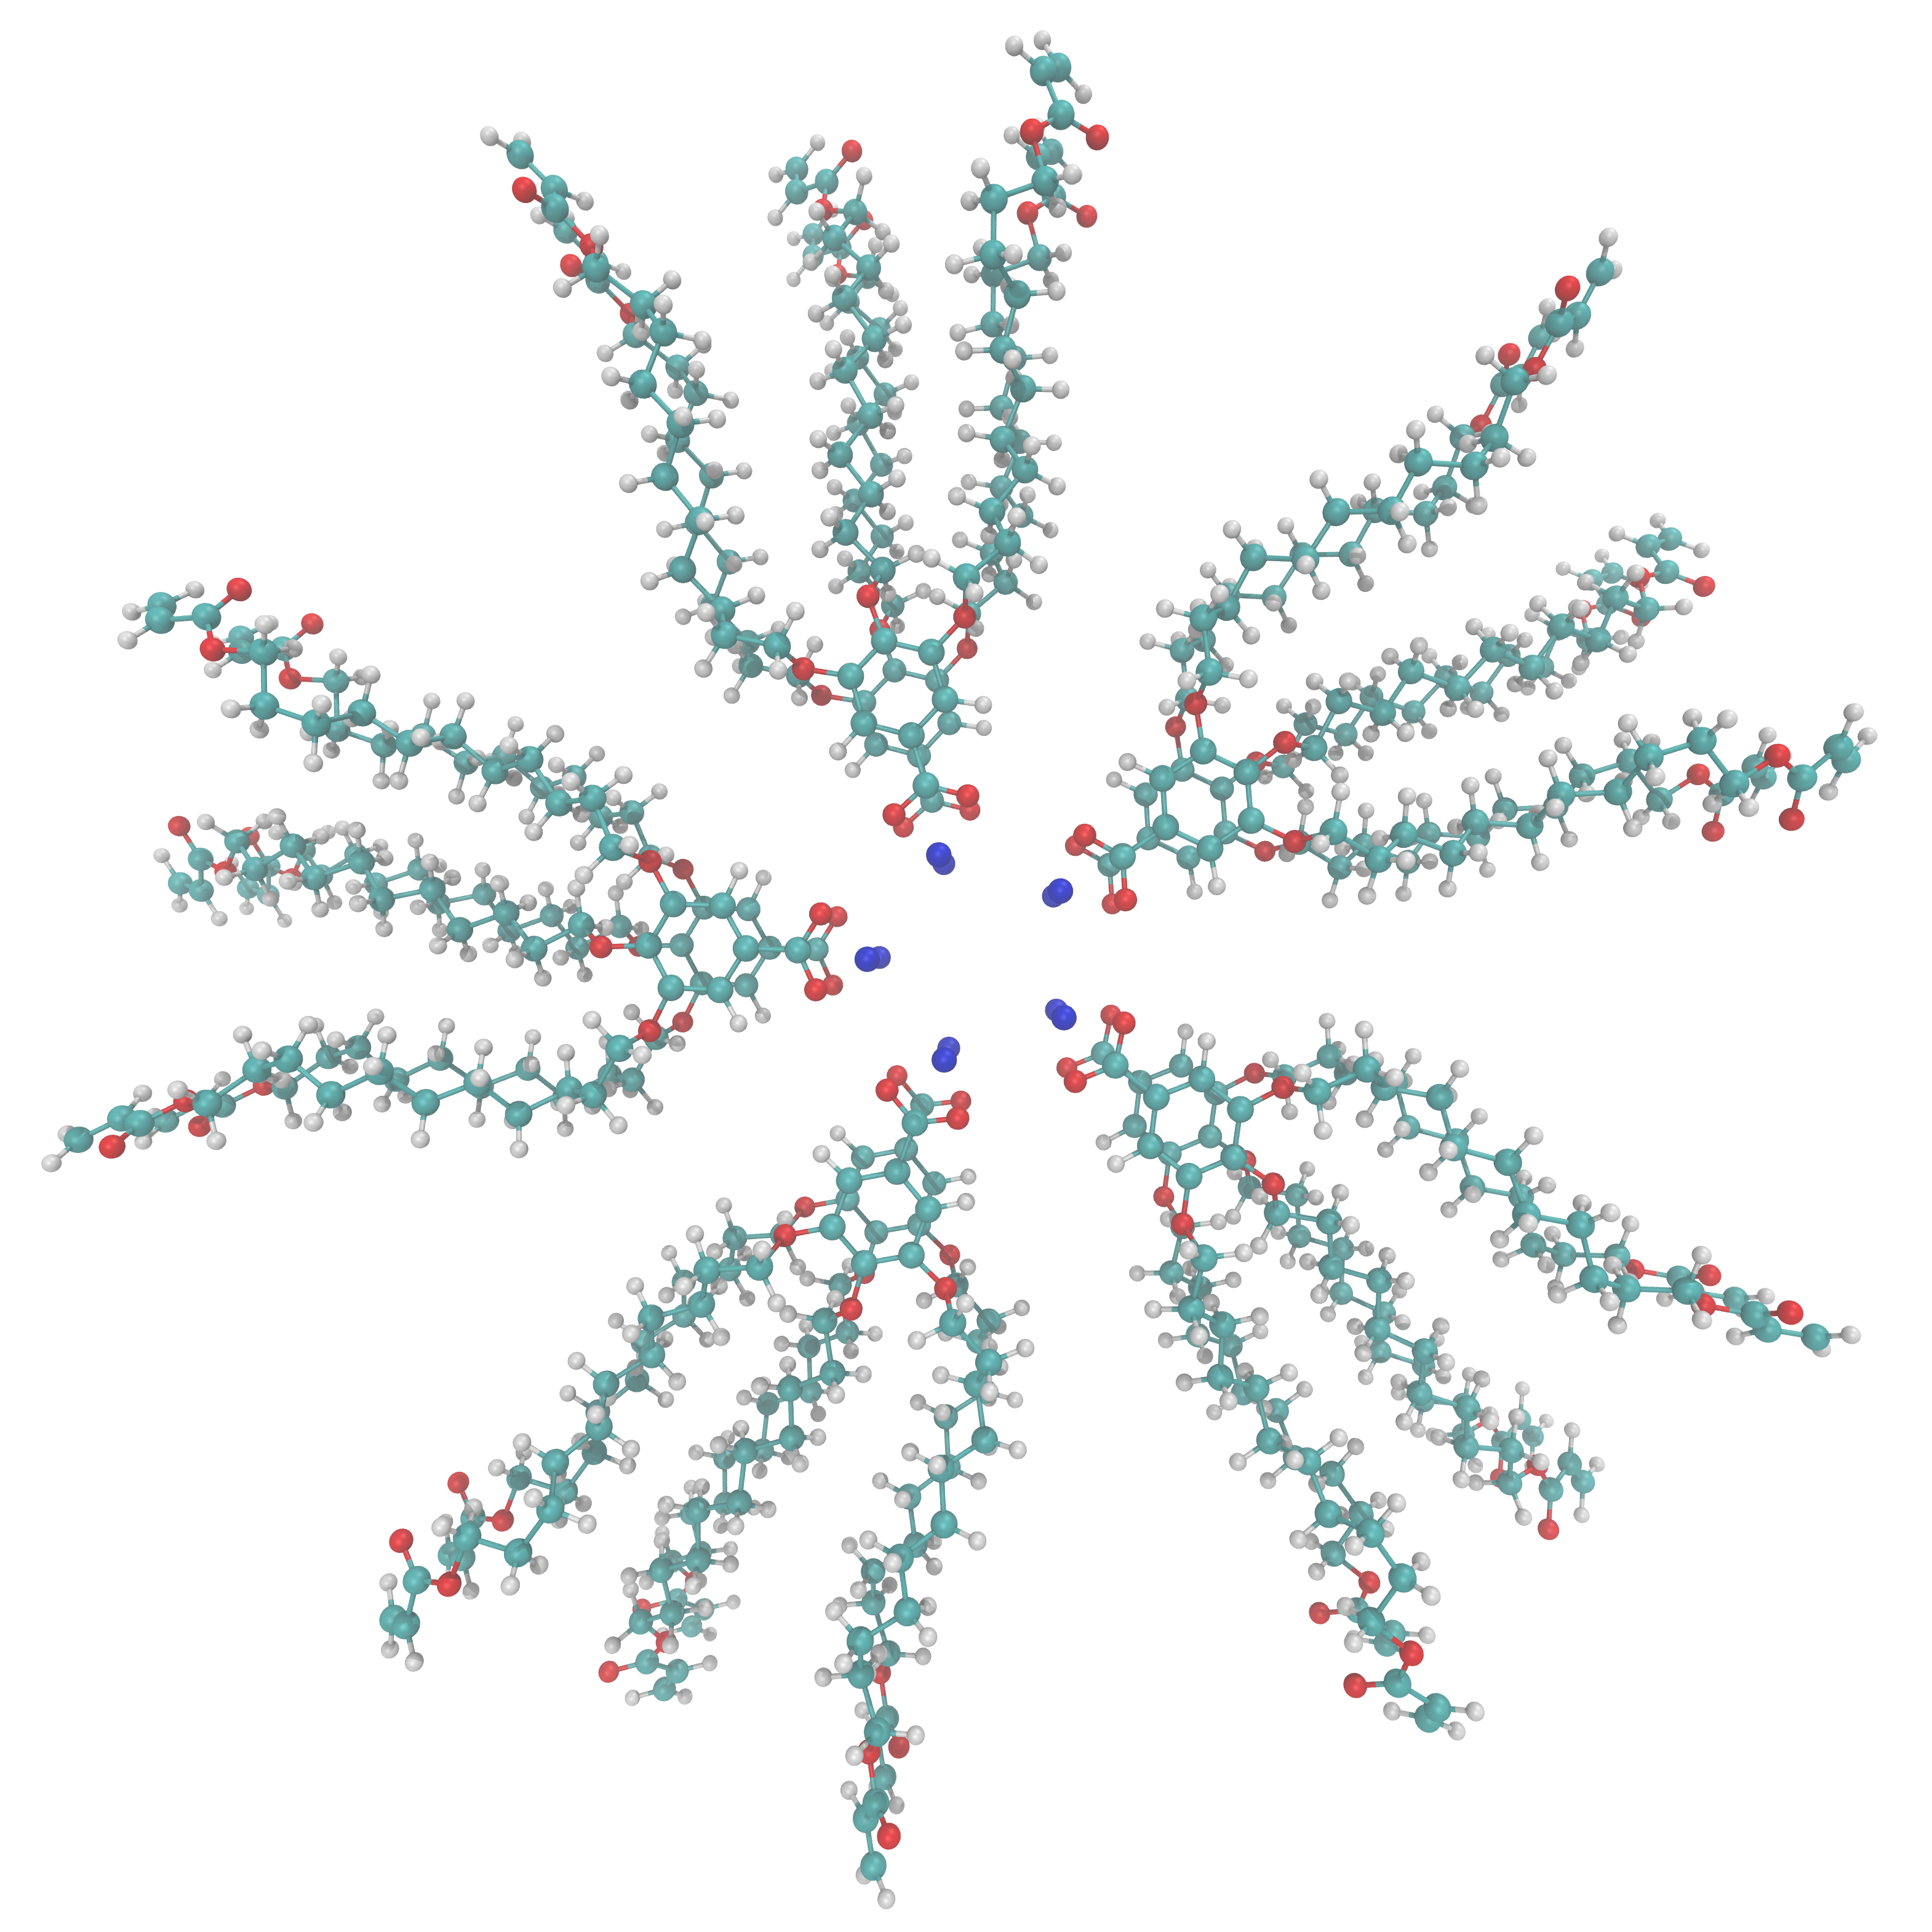
\includegraphics[width=\textwidth]{sandwichedlayers.png}
%		\caption{}\label{fig:sandwichedlayers}
%	\end{subfigure}
%	\begin{subfigure}[b]{0.475\textwidth}
%		\centering
%		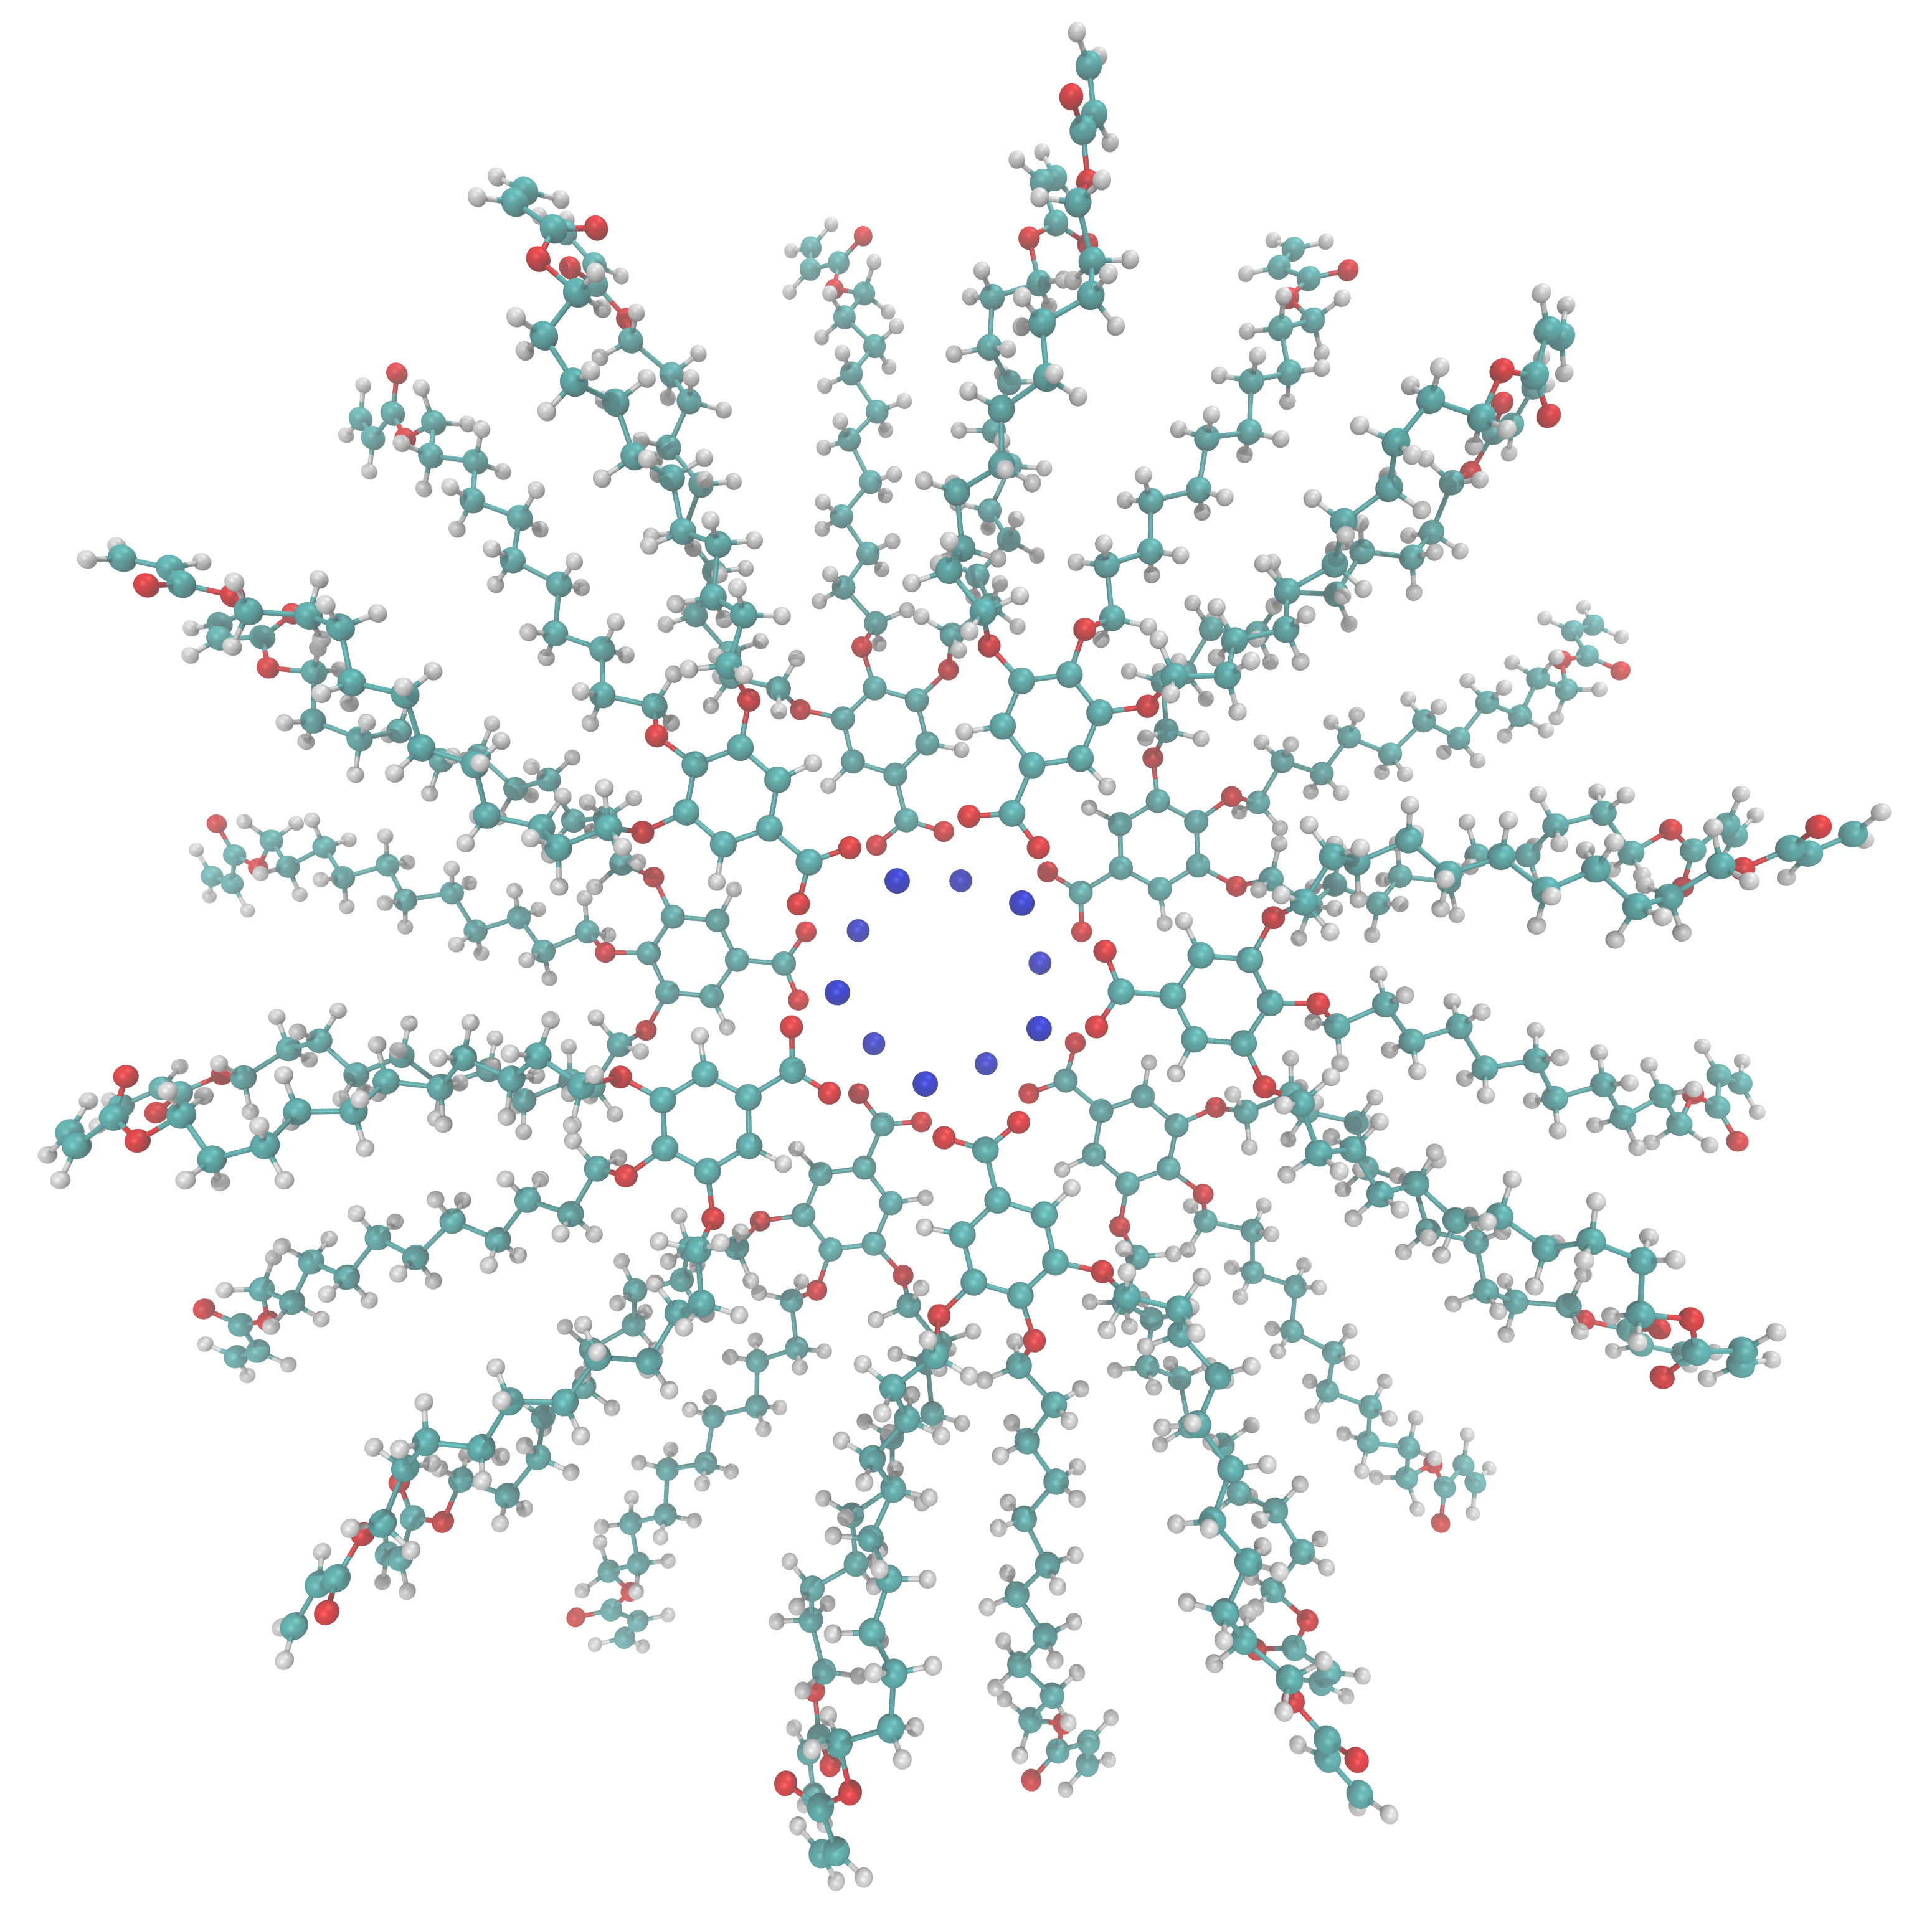
\includegraphics[width=\textwidth]{offsetlayers.png}
%		\caption{}\label{fig:offsetlayers}
%	\end{subfigure}
%	\caption{(a) Sandwiched benzene dimers stack 3.8 \angstrom~apart. (b) Parallel-Displaced benzene dimers stack
%	3.4 \angstrom~vertically and 1.6 \angstrom~horizontally apart. (c) T-shaped benzene dimers stack 5.0 \angstrom~apart. 
%	(d) Two monomer layers stacked in the sandwiched configuration (e) Two monomer layers stacked in the parallel-displaced
%	configuration }\label{fig:stacking}
%  \end{figure}
  
  We explored the pore composition by measuring the average number densities of
  various monomer components as a function of distance from the pore centers. We
  looked at the average number density of sodium ions, aromatic rings and carbon
  atoms making up the monomer tails. We binned the radial distance of all atoms
  in each group from the pore centers, then normalized by the volume of the
  annulus defined by the bin edges and z box vector.
  %BJC: Maybe write an equation here? It's hard to say precisely how I did it
  %in words without it sounding confusing 

  We calculated ionic conductivity using two different methods for robustness.
  The Nernst-Einstein relation relates the DC ionic conductivity to ion
  diffusivity, $D$, concentration, $C$, ion charge, $q$, the Boltzmann constant,
  $k_b$, and temperature, $T$: $$\sigma = \dfrac{q^2CD}{k_b T}$$ 
  We measured sodium ion diffusion coefficients by calculating the slope
  of the linear region of the z-direction mean square displacement curve as
  indicated by the Einstein relation \cite{einstein_investigations_1956}. We
  visualized the MSD plot to determine where to begin and end a linear fit. We
  measured ion concentration with respect to the volume of the entire unit cell. 

  The second method, termed the Collective Diffusion model, measures the
  movement of the collective variable, Q, which is defined as the amount of
  charge transfer through the system and can be thought to represent the center
  of charge of the system. The conductance, $\gamma$, of the system can be
  calculated as: $$ \gamma = \dfrac{D_Q}{k_b T} $$ We convert the resulting value
  to ionic conductivity by multiplying by channel length and dividing by the
  membrane cross sectional area. $D_Q$ is the diffusion coefficient of the
  collective variable Q. It is calculated using the Einstein relation. One can
  access a full derivation of the model elsewhere \cite{liu_collective_2013}.

  \section{Results and Discussion}
  
  \subsection{Determining the Number of Monomers per Layer}

  Our simulations best support a model built with 5 monomers per layer based on
  the measured equilibrated pore-to-pore distances. To discern the composition of
  the monomer layers, addressing (\ref{point:monomernum}), we ran simulations of
  systems created with 4 - 8 monomers per layer. We built systems in both the
  parallel displaced and sandwiched configurations with layers initially spaced
  3.7 \AA~apart. We prepared equilibrated configurations according to the dry
  equilibration procedure. All systems are stable after 400 ns of simulation. In
  a sense, all systems are at least metastable, addressing
  (\ref{point:metastable}), however not all will make physical sense or fit the
  experimental profile that we are looking to match. Figure~\ref{fig:p2p} shows
  the pore spacing for all systems tested. Systems built with 5 monomers in each
  layer equilibrate to a pore spacing that is most consistent with the
  experimental value of 4.12 nm derived from SAXS measurements
  (Figure~\ref{fig:SAXS}). The remainder of this discussion will focus on the
  analysis of systems built with 5 monomers per layer.

  \begin{figure}
	\centering
	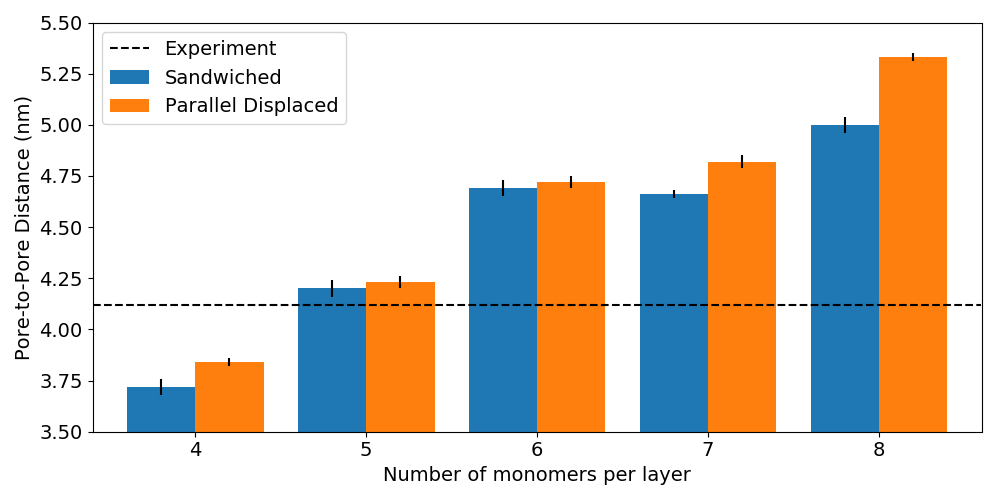
\includegraphics[width=\linewidth]{p2p.png}
	\caption{When we build systems with 5 monomers per layer in the
		parallel displaced configuration, the equilibrated pore spacing is closest to
		the experimental value of 4.12 nm. The equilibrated pore spacing of the model
		increases as the number of monomers in each layer increases. The pore spacing
		of systems starting in the sandwiched configuration is systematically slightly
		lower than those started in the parallel displaced configuration.}~\label{fig:p2p}
  \end{figure}  

  \subsection{Layer partitioning}

  We learned that layers are well-defined and persistent, answering
  (\ref{point:layers}). We established our conclusion by plotting the one dimensional pair
  distribution function, $g(z)$, calculated between atoms along the length of the
  pores (Fig.~\ref{fig:zdf}). We measured $g(z)$ with respect to aromatic rings in
  the head groups and, separately, with respect to carbon atoms in the alkane
  chains. Using a Fourier transform of $g(z)$, we see that sandwiched
  configuration layers stack 4.39 \angstrom~apart while parallel displaced
  configuration layers stack 4.38 \angstrom~apart.

  Insert paragraph about 2D pair distribution function (yz cross section). 

  We measured the correlation length, L, by fitting a function of the form:
  $$1 + Asin(Bx + C)e^{-z/L}$$ where z is the independent variable and all
  other variables are fitting parameters. The correlation length for each
  system is given in Table~\ref{fig:correlation_length}.

  \begin{table}[h]
  \centering
  \begin{tabular}{ccc}
  \toprule
  System & Layer Separation & Correlation Length \\
  \midrule
  Sandwiched & 4.39 \AA & 41 $\pm$ 3 \AA \\
  Parallel Displaced & 4.38 \AA & 86 $\pm$ 14 \AA \\
  Experiment* & 3.7 \AA & 32 $\pm$ 1 \AA \\  
  \bottomrule
  \end{tabular}
  \caption{*See supplemental information for derivation of experimental correlation length}~\label{fig:correlation_length}
  \end{table} 

  %BJC: TODO: increase font size on legends
  \begin{figure}
        \centering
        \begin{subfigure}{0.45\textwidth}
                \centering
                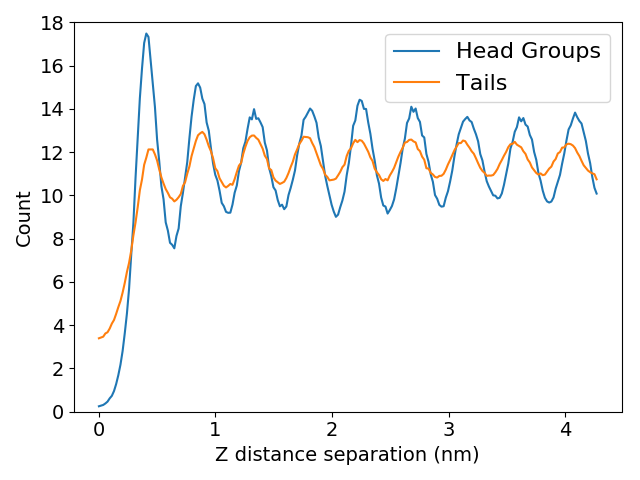
\includegraphics[width=\textwidth]{zdf_overlay_layered.png}
                \caption{}\label{fig:zdf_layered}
        \end{subfigure}
        \begin{subfigure}{0.45\textwidth}
                \centering
                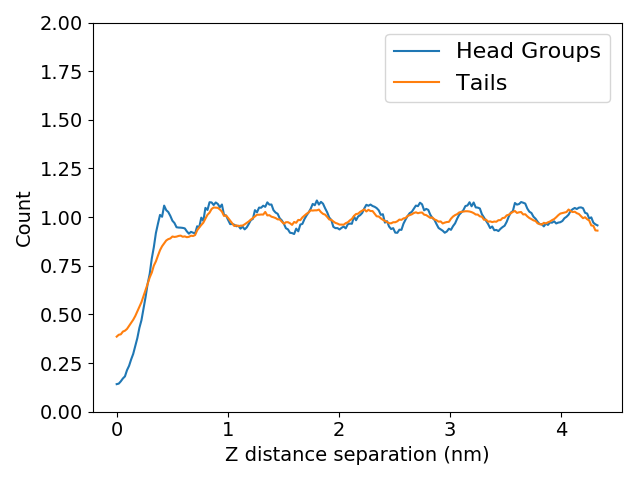
\includegraphics[width=\textwidth]{zdf_overlay_offset.png}
                \caption{}\label{fig:zdf_offset}
        \end{subfigure}
	\caption{We support the existence of layers with the observance of
		clear periodic maxima in the $z$-direction pair distribution functions of the
		(a) 5 monomer per layer, sandwiched and (b) 5 monomer per layer, parallel
		displaced configurations. The extent to which we consider a system to be
		layered is based on the magnitude of the deviation of the periodic maxima from
		the average number density. The sandwiched configuration possesses a higher
		degree of layering than the parallel displaced configuration and, in both
		cases, the head group region has a higher degree of layer partitioning than the
		tail region. (See supplemental information for detailed definitions of the head
		group and tail regions)}\label{fig:zdf}
  \end{figure}

  \subsection{Determination of Relative Interlayer Head Group Orientation}

  We answer question (\ref{point:orientation}) by simulating X-ray diffraction
  patterns produced from equilibrated MD trajectories. We tested systems built
  with 5 monomers per layer in the parallel displaced and sandwiched
  configurations. We generated simulated patterns using portions of simulation
  trajectory after equilibration. The patterns for both structures are shown and
  compared to experiment in Figure \ref{fig:XRDsim}.

  Simulated XRD of the sandwiched configuration contains all experimental
  features except for R-helix. R-alkanes, R-spots and R-pores appear close to their
  expected locations. R-$\pi$ is also present, however it intersects R-alkanes at
  a $q_z$ value lower than experiment meaning the head groups in our model prefer 
  to stack farther apart. 

  The parallel displaced configuration results in a simulated XRD pattern with
  the closest match to experiment. It produces the only pattern that exhibits all
  major reflections. R-alkanes and R-pores appear as they do in the sandwiched
  configuration. R-spots and R-$\pi$ appear, however with a lower intensity
  relative to R-alkanes when compared to the sandwiched configuration. R-helix
  appears due to the parallel displaced aromatic rings. It is a subharmonic of
  R-$\pi$ since the nearest vertically stacked head group to any given head group
  is 7.4 \AA~away. 

  %BJC: adjust figure size and alignment -- probably easiest to set figure size in matplotlib
  \begin{figure}
  \begin{subfigure}{0.3\linewidth}
        \centering
        \vspace{-0.2em}
        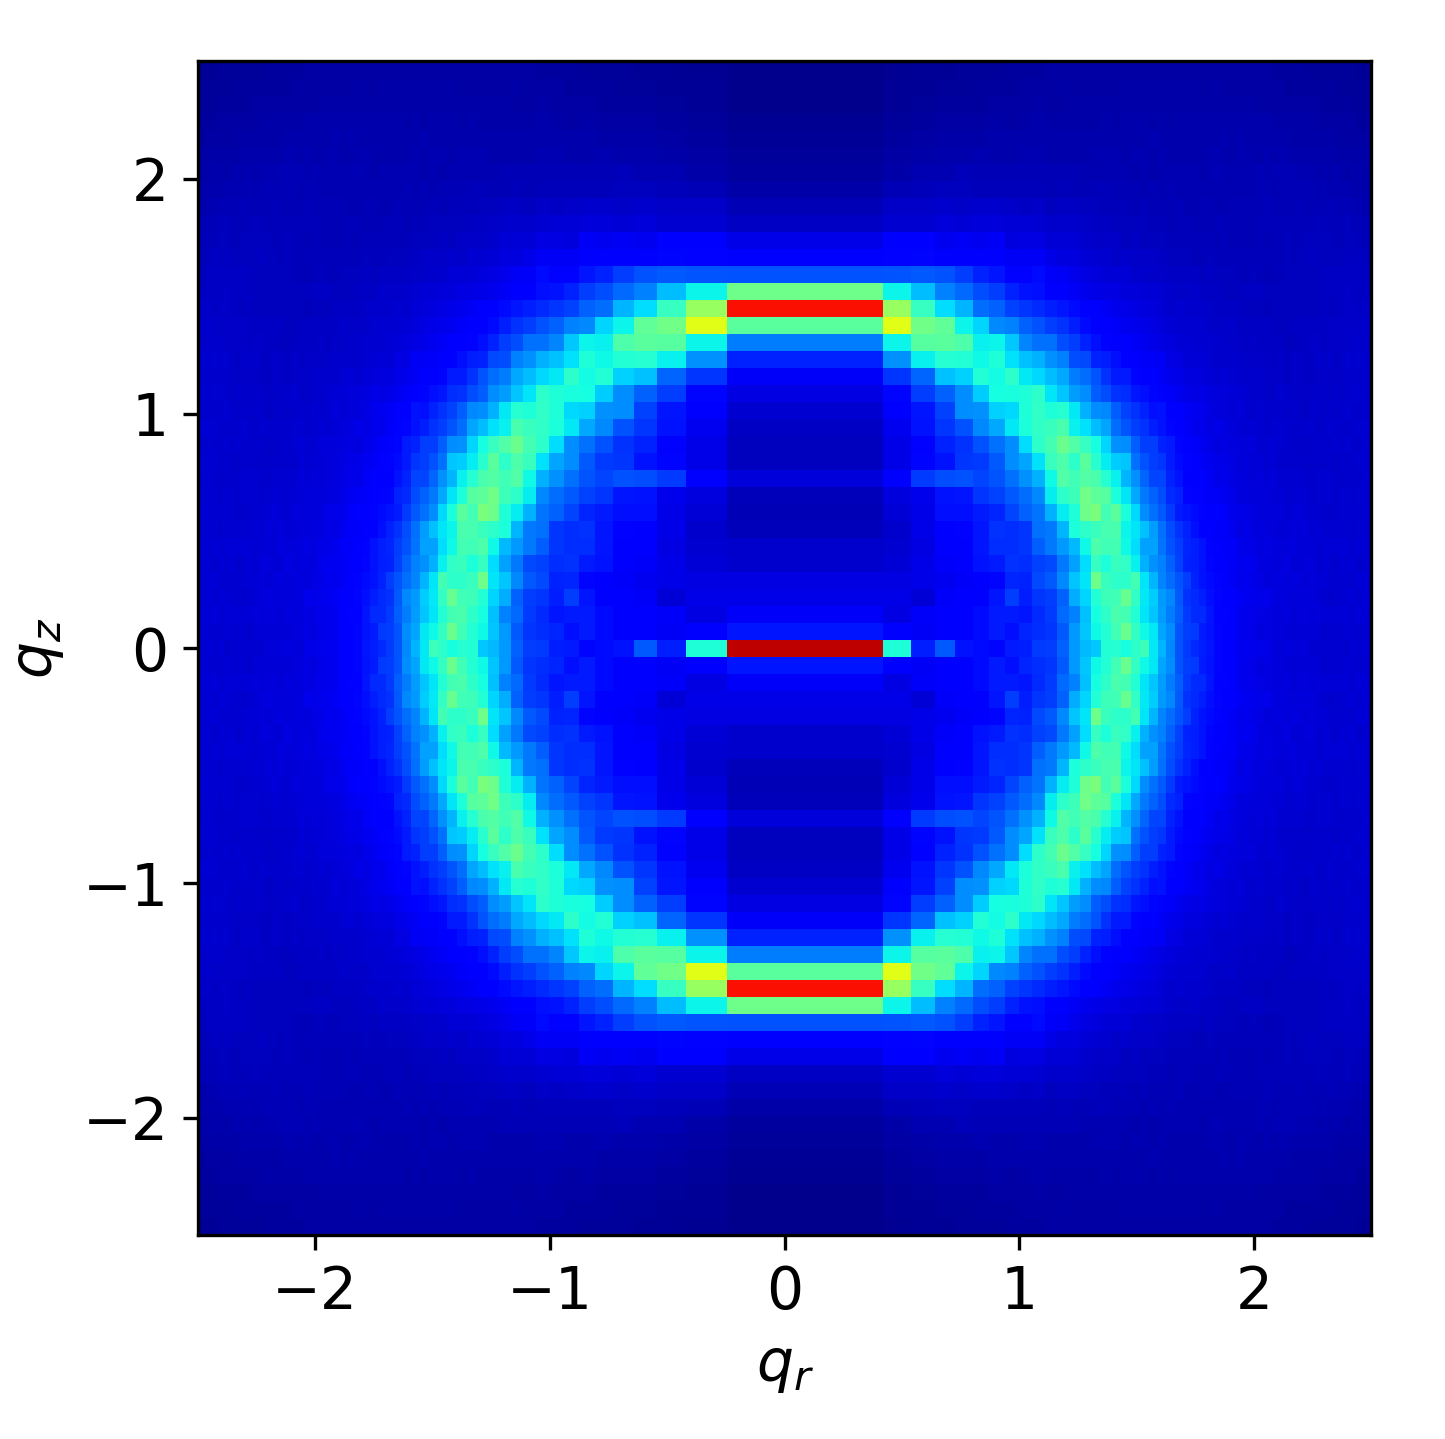
\includegraphics[width=1.018\linewidth]{offset_rzplot.png}
        \caption{}~\label{fig:rz_offset}
  \end{subfigure}
  \begin{subfigure}{0.3\linewidth}
        \centering
%        \vspace{0.25em}
        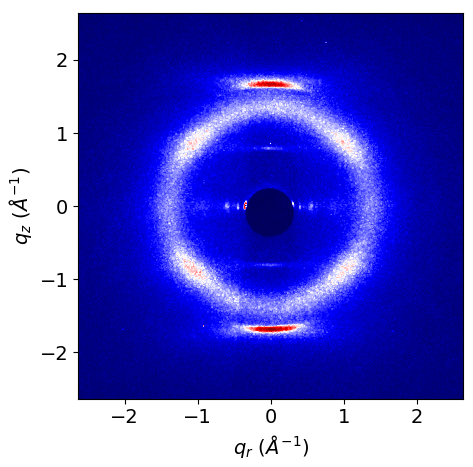
\includegraphics[scale=0.29]{WAXS_raw.png}
        \caption{}~\label{fig:raw_waxs}
  \end{subfigure}
  \begin{subfigure}{0.3\linewidth}
        \centering
        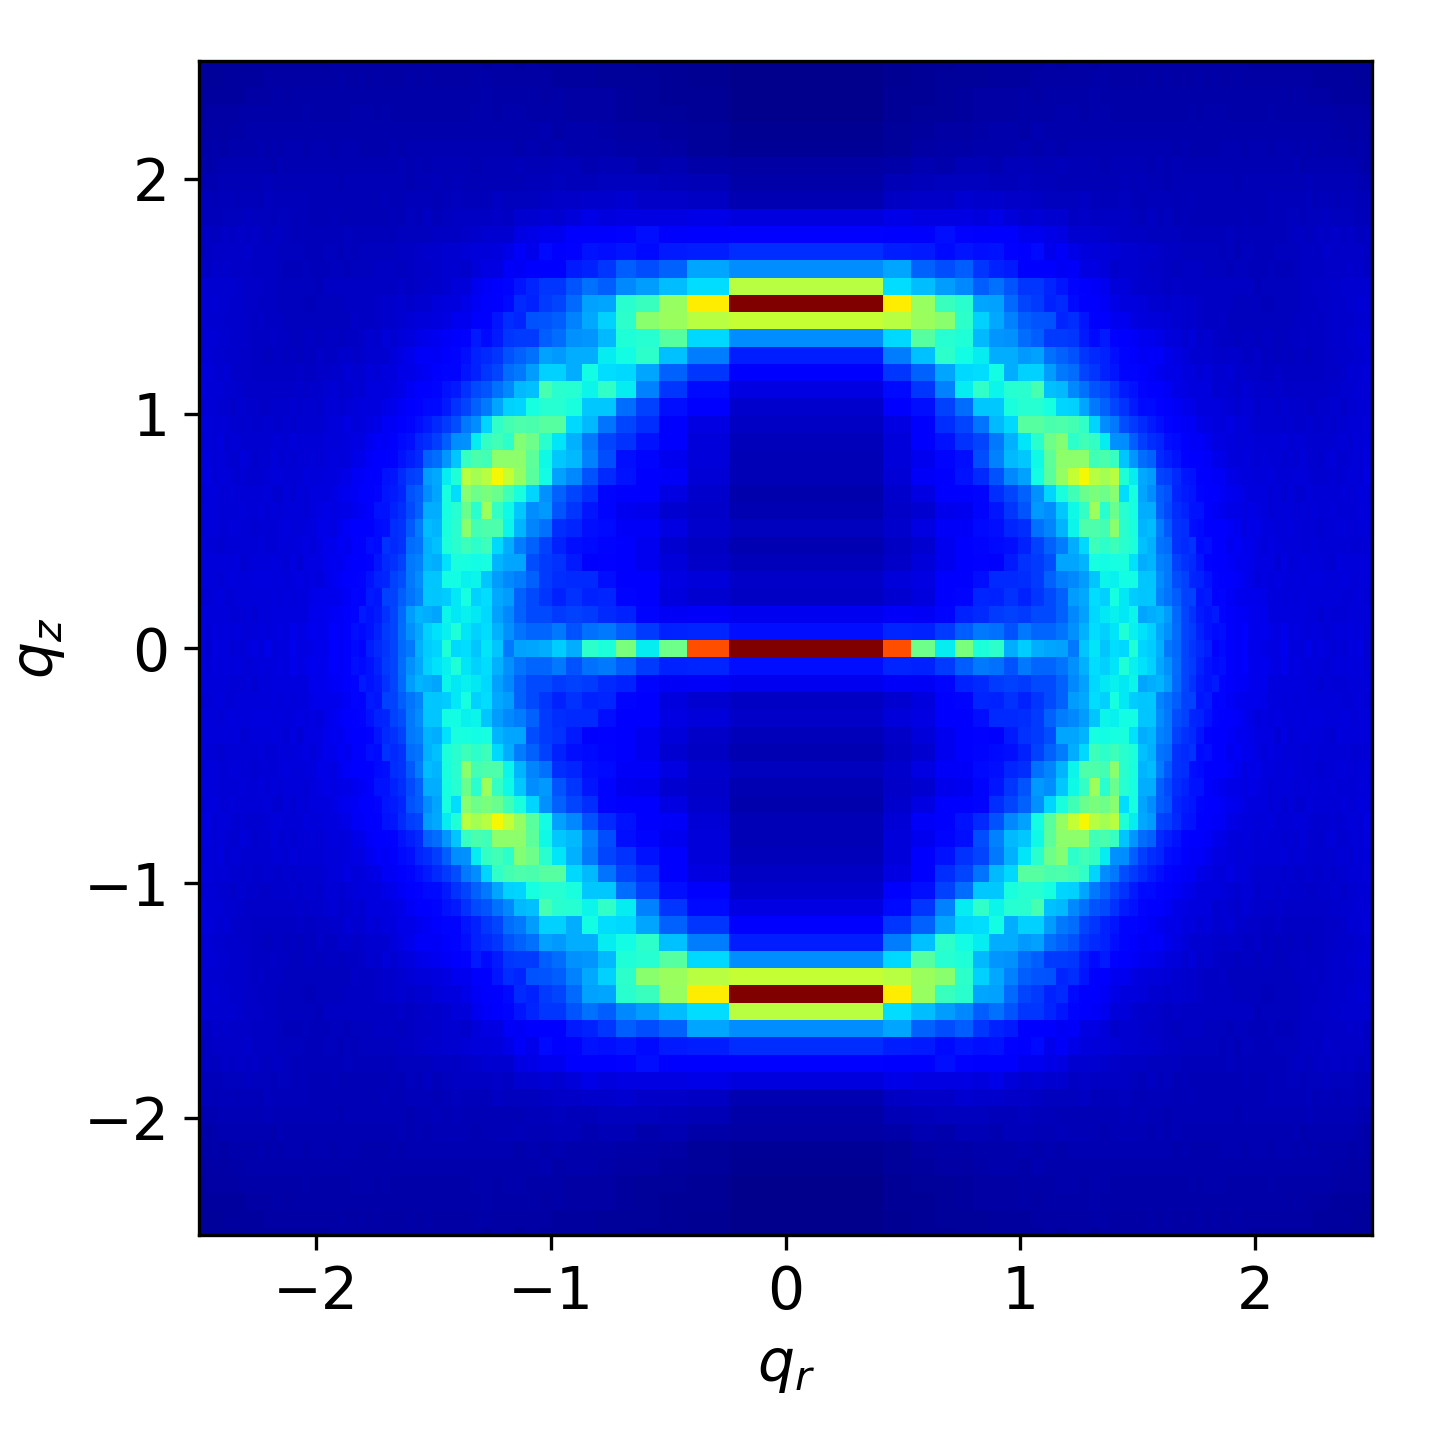
\includegraphics[width=\linewidth]{layered_rzplot.png}
        \caption{}~\label{fig:rz_layered}
  \end{subfigure}
  \begin{subfigure}{0.0544\linewidth}
        \centering
        \vspace{-4.00em}
        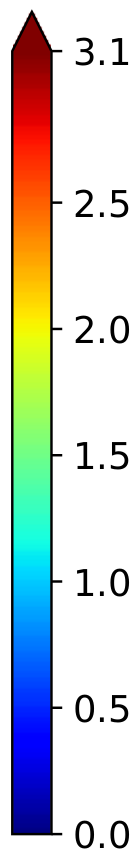
\includegraphics[width=\linewidth]{colorbar_jet.png}
  \end{subfigure}
  \caption{The simulated XRD pattern generated from the equilibrated trajectory
	  of the parallel displaced configuration (a) exhibits all major reflections
	  present in the experimental WAXS pattern (b). The simulated XRD pattern
	  generated from the equilibrated trajectory in the sandwiched configuration shows
	  all major reflections except R-helix.}
  \label{fig:XRDsim}
  \end{figure}

%  In both simulated diffraction patterns R-alkanes appears in the expected location. 
%  The location of R-pores is not well-defined in comparison to experiment. In order
%  to resolve those reflections it would be necessary to simulate a much larger system, 
%  but that is unnecessary since we can measure pore spacing manually as described 
%  earlier. R-$\pi$ and R

  In both the parallel displaced and sandwiched configurations, we noted that
  R-$\pi$ appears in a location which corresponds to a real space separation
  larger than experiment. We attribute this discrepancy to GAFF's inability to
  appropriately model the aromatic interactions which would be necessary to
  achieve the correct $\pi$-$\pi$ stacking distance. 
  %Systems have been modeled that exhibit the correct stacking distance, however
  %they are typically made of planar molecules spanning a large area.
  %BJC: I saw a paper like this a long time ago, but failed to save the citation and
  % now I am having a hard time finding it again. 
  The system we have modeled has bulky tails whose entropic contributions compete
  with the $\pi$-$\pi$ stacking interaction energy. There have been efforts to
  model systems that contain $\pi$ interactions in a classical mechanical context
  using polarizable forcefields \cite{baker_polarizable_2015}. We could
  implement a polarizable force field, however it is likely not worth the extra
  computational cost. If our model proves to be inadequate when simulating
  transport, we will revisit our current choice of forcefield.  

  The R-spots signal, which appears in both simulated XRD patterns, is a result
  of hexagonal alkane chain packing. Previous literature has explained the spots
  in the diffraction pattern as the product of tilted alkane chains. We measured
  the tilt angle of the alkane chains and showed that our system equilibrates to
  an average tilt angle close to zero degrees (Fig.~\ref{fig:tilt}). To
  understand the origin of the spots, we determined which atoms gave rise to the
  feature. Since R-spots is present as higher intensity spots within R-alkanes,
  it is likely that the spots arise as a consequence of the tails. By removing
  all non-tail atoms from the trajectory and simulating a diffraction pattern, we
  were able to isolate the cause of the spots to the tails
  (Figure~\ref{fig:tails}). Since the tails stay nearly flat, we plotted the
  centroids of the tails and measured the angle between each centroid and its
  nearest neighbors with respect to the plane of the membrane. We see distinct
  peaks in the distribution of these angles (Figure~\ref{fig:tail_packing}).

  \begin{figure}
  \centering
  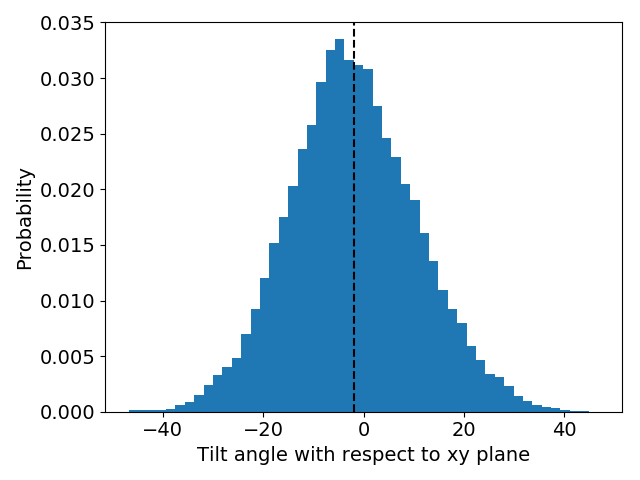
\includegraphics[width=0.5\linewidth]{tilt_dist.png}
  \caption{We measured the angle made between each monomer alkane tail and the membrane plane. 
  The average tilt angle is near 7\degree~which is far from the 37\degree~tilt angle 
  previously used to explain R-spots.}~\label{fig:tilt}
  \end{figure}

  The peaks in the nearest neighbor angle distribution are consistent with the
  location of R-spots. The peaks of interest in Figures \ref{fig:offset_tails}
  and \ref{fig:layered_tails} are located at $\pm 33 \degree$ which is the same
  location where the highest intensity of spots are located on the simulated
  patterns. We confirmed this conclusion by radially integrating the 2D WAXS
  pattern for $\left|\mathbf{q}\right|$ values between 1.4 and 1.57 (between 4
  and 4.5 \AA~in real space). We observe that distinct peaks appear ca. $30
  \degree$, in close agreement with the previously measured angle distribution
  (Figs.~\ref{fig:offset_integration}~and~\ref{fig:layered_integration}). We
  performed the same integration on the raw experimental data and found the angle
  at which R-spots reaches its highest intensity to be $\pm 37 \degree$ which
  is a reconcilable difference with our simulated results.  

  \begin{figure}
	\centering
	\begin{subfigure}{0.45\linewidth}
		\centering
	 	\vspace{-2em}
		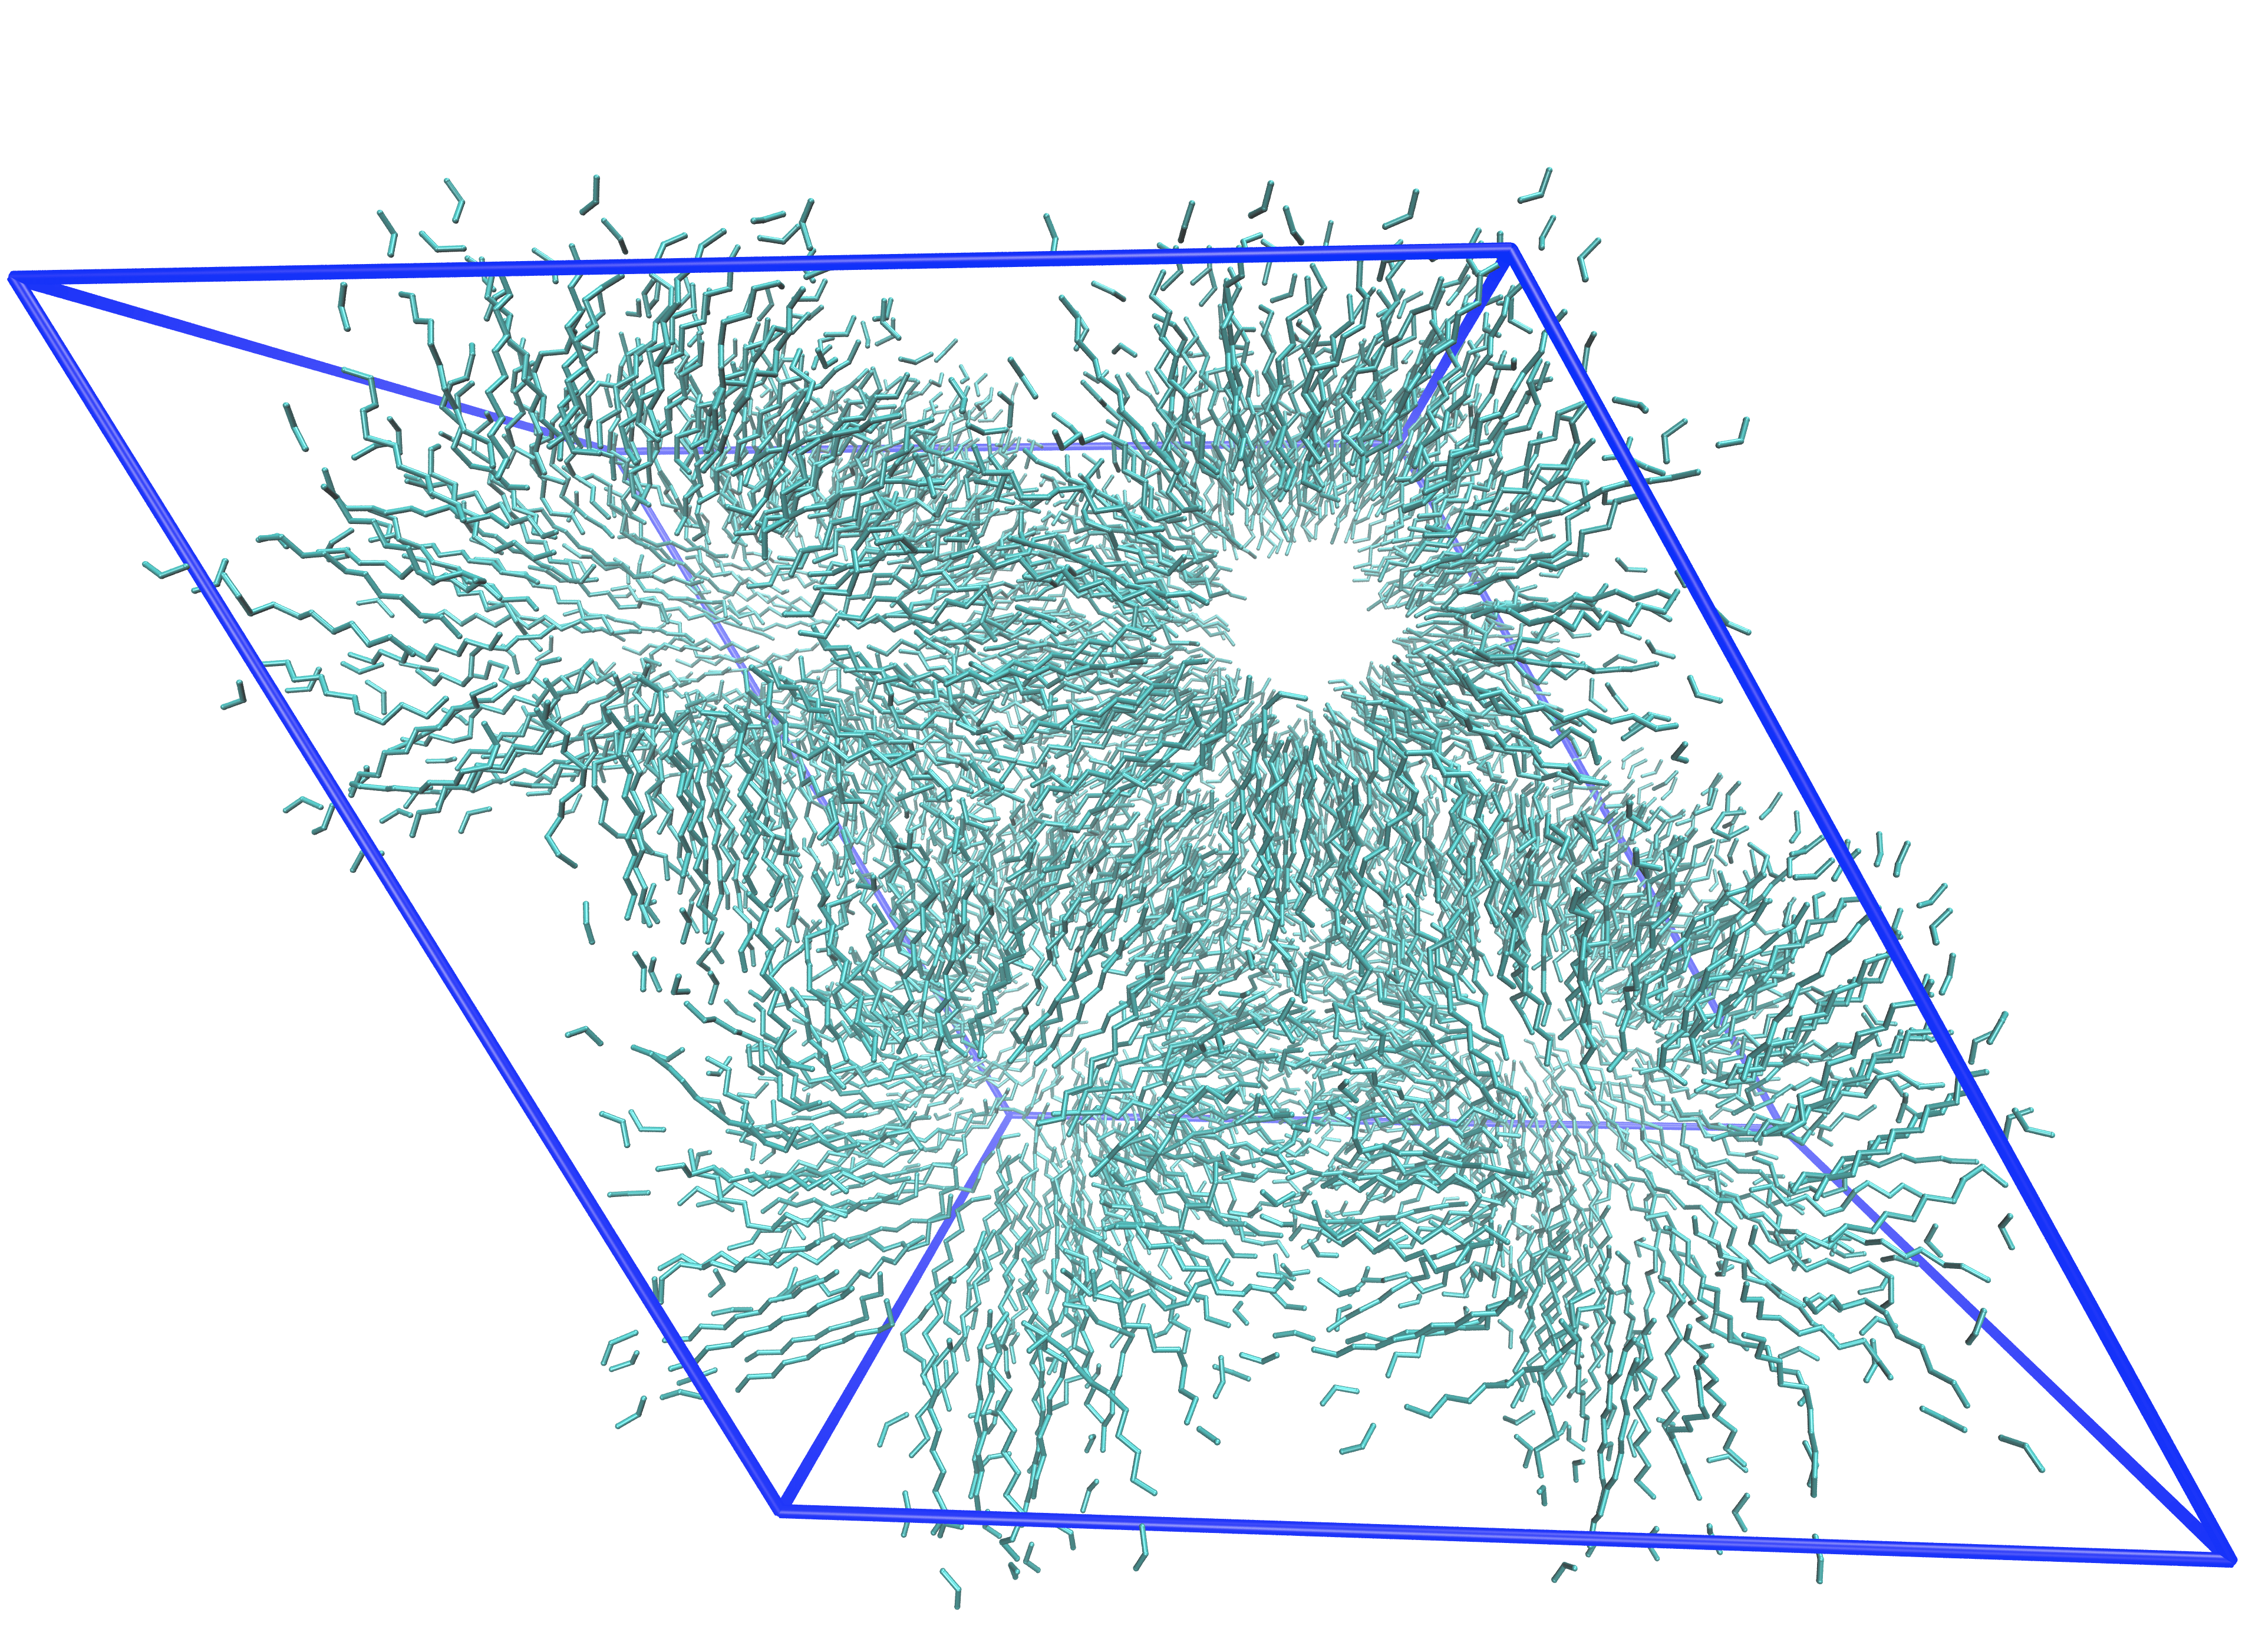
\includegraphics[width=\textwidth]{tails_topview.png}  % picture of top of unit cell with only tail atoms shown
		\caption{}\label{fig:topdown_tails_only}
	\end{subfigure}
	\begin{subfigure}{0.45\linewidth}
		\centering
		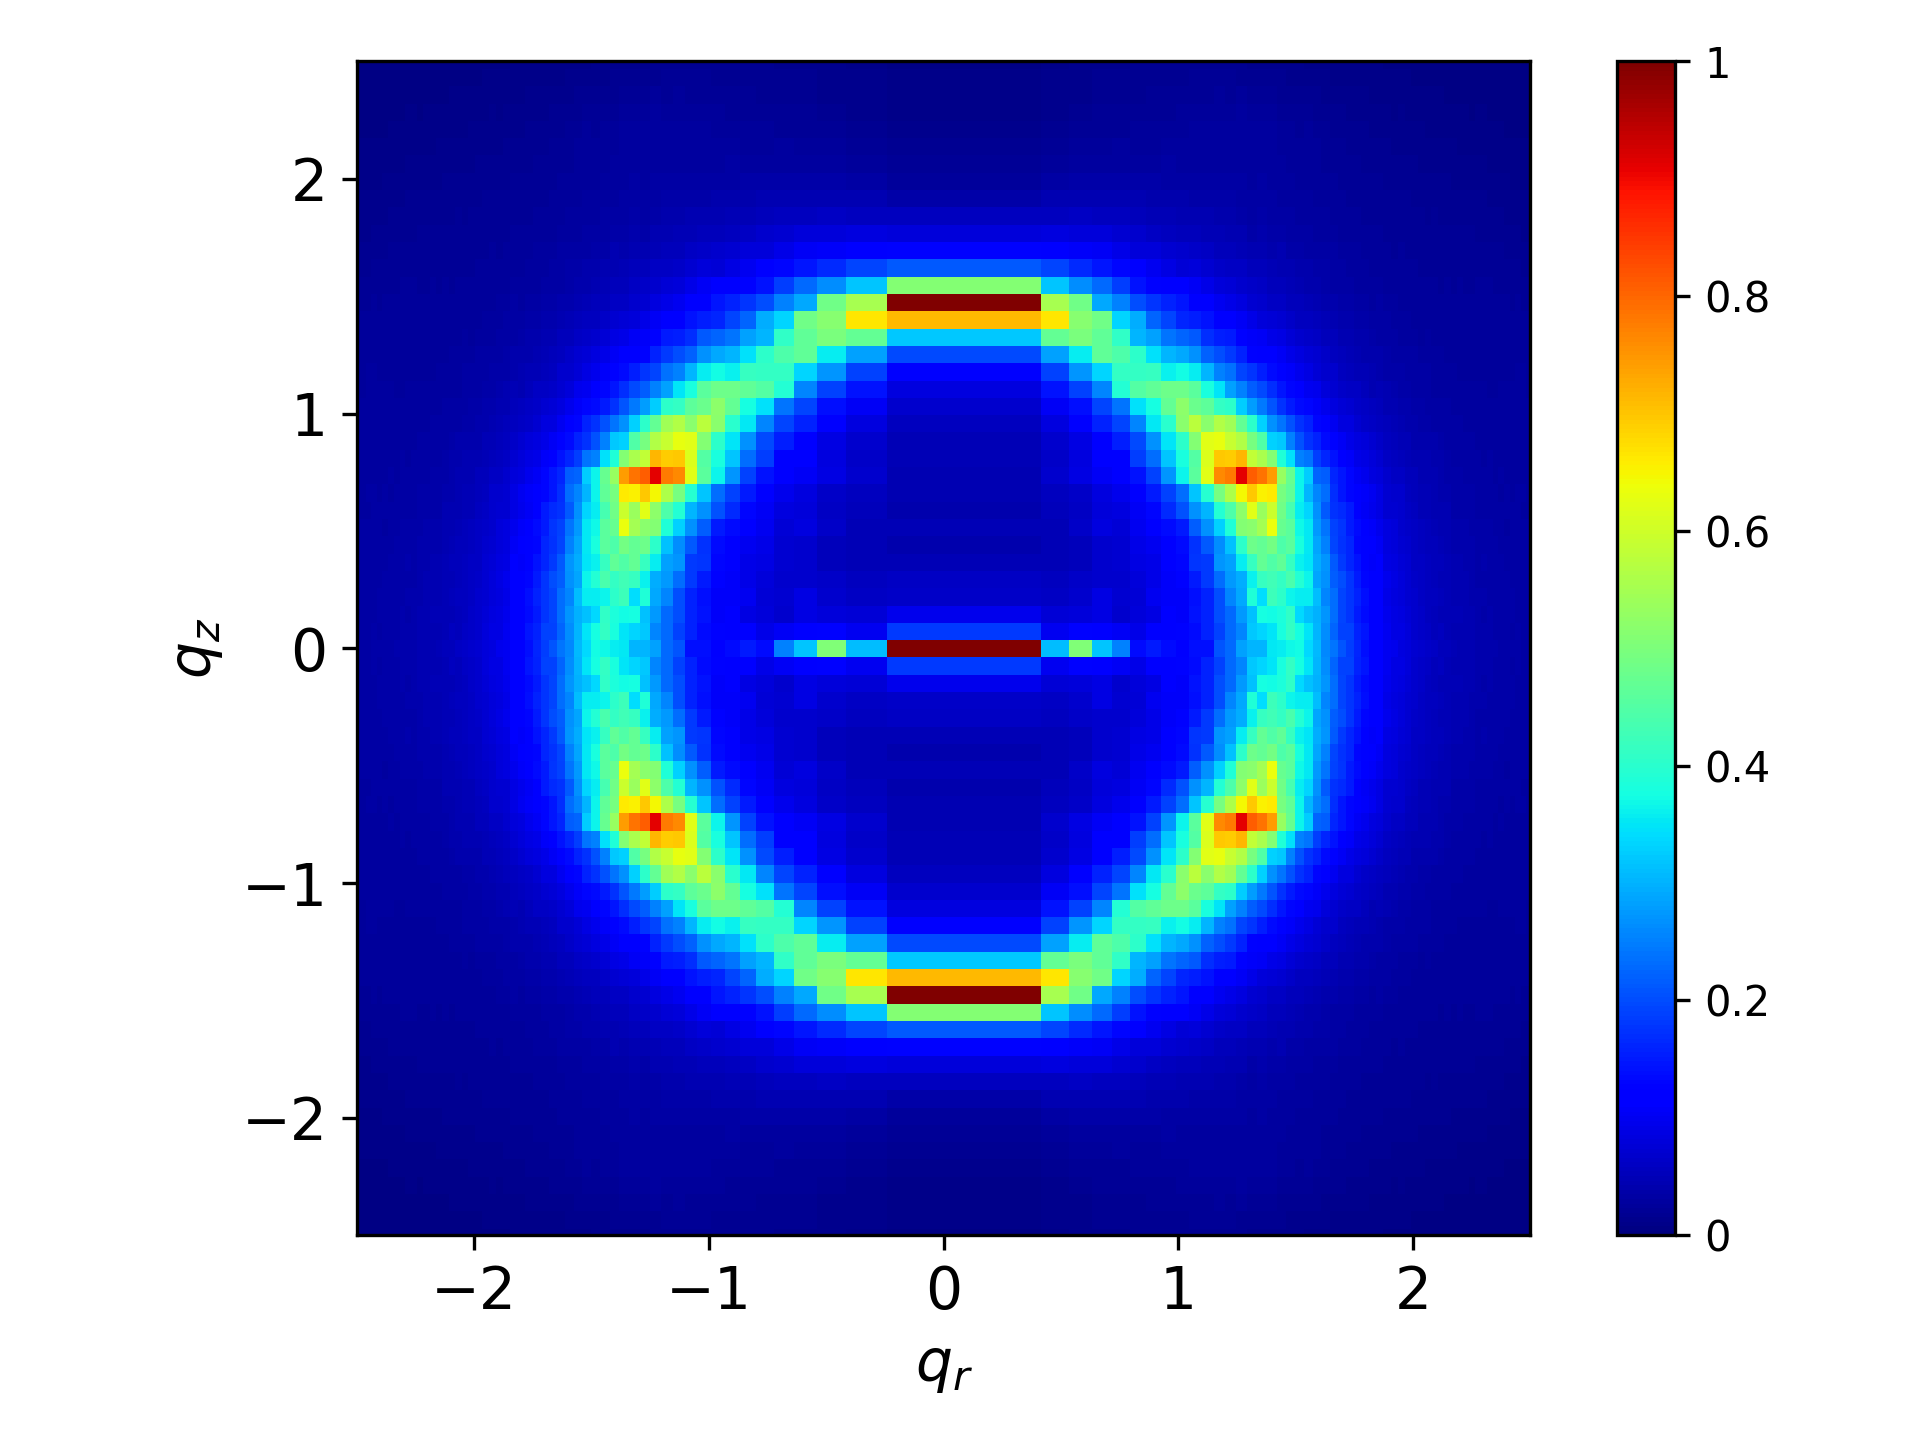
\includegraphics[width=\textwidth]{tails_rzplot.png}
		\caption{}\label{fig:tails_rzplot}
	\end{subfigure}
	\caption{(a) We removed all atoms except carbon atoms that constitute the tails from a 
	sandwiched configuration trajectory. (b) The simulated XRD pattern of the
        tail-only trajectory still shows R-spots}\label{fig:tails}
        %MRS3: so I didn't realize this before, but why are there still fairly significant peaks in the pi-stacking region when the head groups are removed?
        %Do you feel you understand this? I suppose it is because the top of the tails must be correlated with the aromatic ring by covalent bonding?
        %BJC2: Yea, I think the reflection is correlated to the aromatic rings. The system shown is the sandwiched configuration. The intensity of "R-pi"
        % in this pattern is lower than in the pattern generated by the full system. The aromatic rings appear to strengthen the reflection. 
        % Also, the system is layered in the z-direction, as we show, so a reflection like that should appear. 
        %MRS4: did you use a different scaling for the color bar here than above? If so, mention.
        %BJC3: The scaling is the same
  \end{figure}

  \begin{figure}[!htb]
  \centering
  	\begin{subfigure}{\linewidth}
	\centering
		\begin{subfigure}{0.45\textwidth}
        		\centering
        		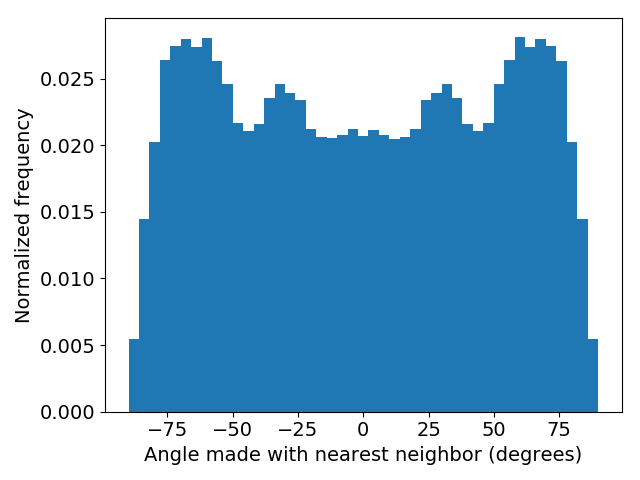
\includegraphics[width=\linewidth]{offset_tail_packing.png}
        		\caption{}~\label{fig:offset_tails}
		\end{subfigure}
		\begin{subfigure}{0.45\textwidth}
		\centering
	        	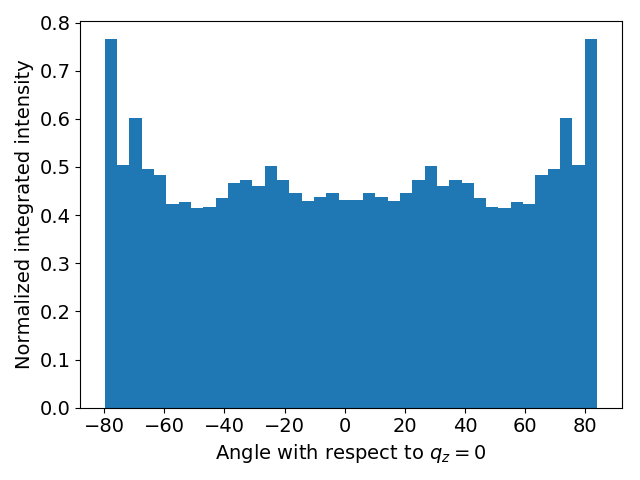
\includegraphics[width=\linewidth]{offset_angle_v_I.png}
		        \caption{}~\label{fig:offset_integration}
		\end{subfigure}
	\end{subfigure}
	\begin{subfigure}{\linewidth}
	\centering
		\begin{subfigure}{0.45\textwidth}
	        \centering
		        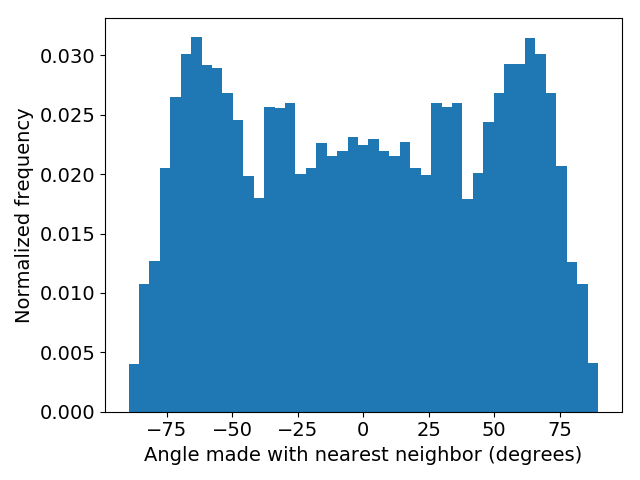
\includegraphics[width=\linewidth]{angles_traj_layered.png}
		        \caption{}~\label{fig:layered_tails}
		\end{subfigure}
		\begin{subfigure}{0.45\textwidth}
        	\centering
		        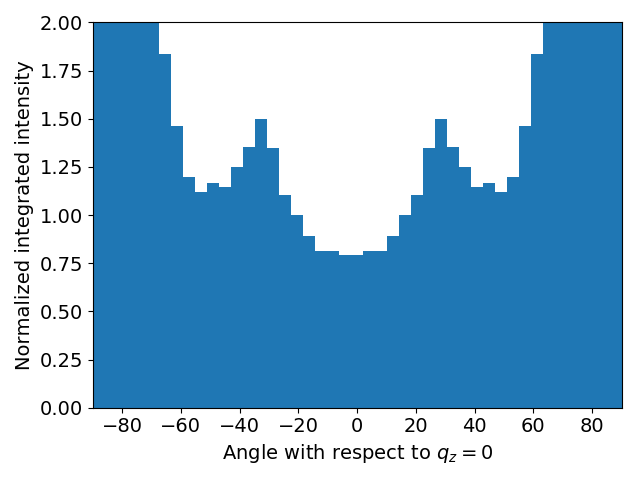
\includegraphics[width=\linewidth]{layered_angle_v_I.png}
		        \caption{}~\label{fig:layered_integration}
		\end{subfigure}
	\end{subfigure} 
  \caption{We hypothesize that R-spots is the result of ordered tail packing.
	  Defining the membrane plane to be 0\degree, we
	  measured the angles between each alkane chain tail centroid and its nearest
	  neighbor centroids for the equilibrated parallel displaced (a) and sandwiched
	  (c) configurations. Peaks that appear in each distribution are centered near
	  $\pm~33\degree$. We radially integrated the simulated XRD patterns of the
	  parallel displaced and sandwiched configuration within the region bounding
	  R-alkanes ((b) and (d) respectively).  Peaks appear in the same location as the
	  angle distributions which corroborates our hypothesis. Further, we note that
	  the peaks are strongest in both plots associated with the sandwiched
	  configuration. As shown in Figure \ref{fig:rz_layered}, systems simulated in
	  the sandwiched configuration exhibit more intense R-spots
	  reflections.}~\label{fig:tail_packing}
  \end{figure}

  \subsection{Initial Layer Spacing Affects System Equilibration}

%MRS4: can we come up with another name?  I still think disordered pores is a decent name, since there is no pi-stacking layering.  ``structures that form when layers are 5 AA apart'' is not so good.  or ``more disordered''?
%BJC3: agreed, I'll stick with disordered pores
%  The $z$-direction correlation functions show that layers in our model prefer
%  to stack further apart than 3.7 \angstrom~as suggested by experiment.
  When we build systems with layers stacked 5.0 \AA~apart and then let them
  equilibrate, we observe long-term stability of a qualitatively different
  configuration, suggesting that we have found another metastable free energy
  basin, further corroborating (\ref{point:metastable}). The basins are
  differentiated by their relative degrees of ordering resulting from different
  spatial arrangements. 

  We expect that the head groups in more ordered systems will be predominantly
  coplanar with the xy plane. We defined a director vector, \textbf{n}, as the
  vector normal to the plane of the monomer's aromatic head group, then measured
  the distribution of angles between it and the z-axis. We used the resulting
  distibution of angles to calculate the nematic order parameter, S. The values
  of S for systems resulting from each initial configuration are presented in
  Table \ref{table:nematic}. The full distributions of angles between \textbf{n}
  and the z-axis are presented in the supplemental material. In general, systems
  started with layers spaced 3.7 \AA apart are more nematically ordered than
  those initially spaced 5 \AA apart. We will refer to systems built with layers
  initially spaced 3.7 \AA apart and 5.0 \AA apart as the ordered and disordered
  pore basins respectively. We studied each basin in both the parallel displaced
  and sandwiched configurations.  

  \begin{table}[h]
  \centering
  \begin{tabular}{cc}
  \toprule
  System & Nematic Order Parameter (S) \\
  \midrule
  Sandwiched, Ordered & 0.659 $\pm$ 0.003 \\
  Parallel Displaced, Ordered & 0.601 $\pm$ 0.003 \\
  Sandwiched, Disordered & 0.565 $\pm$ 0.002 \\
  Parallel Displaced, Disordered & 0.503 $\pm$ 0.002 \\
  \bottomrule
  \end{tabular}
  \caption{The nematic order parameter is higher when layers are initially spaced
  3.7 \AA apart. A perfectly stacked system with aromatic rings coplanar with the
  xy plane would have a nematic order parameter of 1, while isotropically aligned
  director vectors would have a nematic order parameter of 0.}~\label{table:nematic}
  \end{table}

  We observe more evidence of disorder in the disordered pore basin when we 
  plot the two dimensional pair distribution function between the centers of 
  mass of monomer head groups. ADD MORE ANALYSIS ONCE CODE IS WORKING HOW I WANT IT

  \begin{figure}
  \begin{subfigure}{1\linewidth}
        \centering
        \begin{subfigure}{0.45\linewidth}
                \centering
                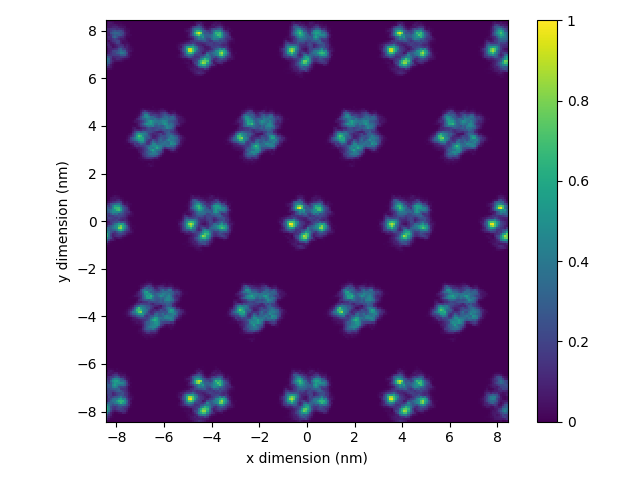
\includegraphics[width=\linewidth]{layered_xy_rings.png}
                \caption{}~\label{fig:sandwich_xy}
        \end{subfigure}%
        \begin{subfigure}{0.45\linewidth}
                \centering
                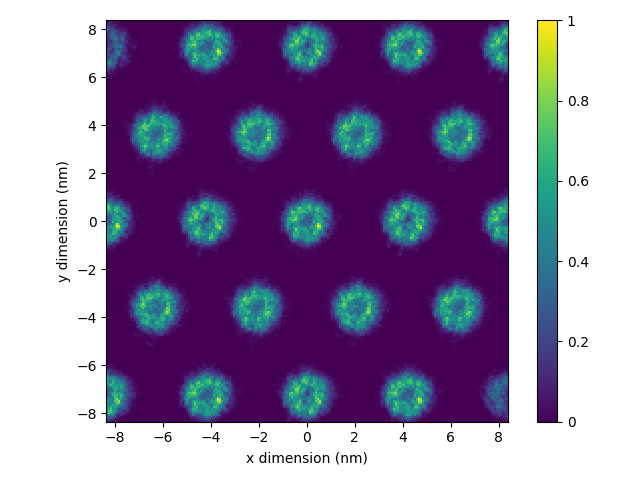
\includegraphics[width=\linewidth]{offset_xy_rings.png}
                \caption{}~\label{fig:offset_xy}
        \end{subfigure}
        \begin{subfigure}{0.45\linewidth}
                \centering
                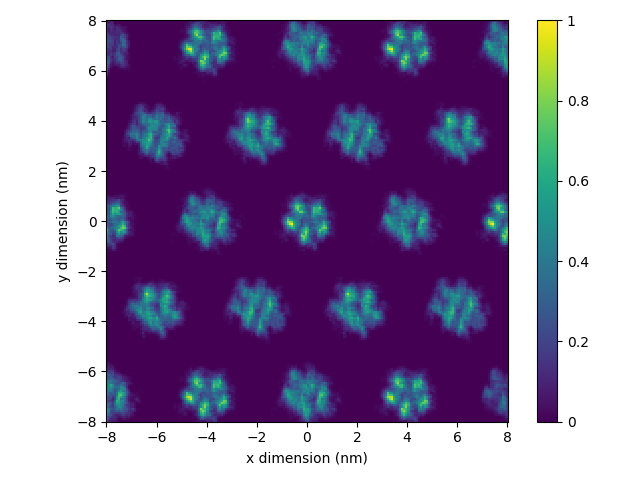
\includegraphics[width=\linewidth]{disorder_sandwich_xy_rings.png}
                \caption{}~\label{fig:disorder_sandwich_xy}
        \end{subfigure}%
        \begin{subfigure}{0.45\linewidth}
                \centering
                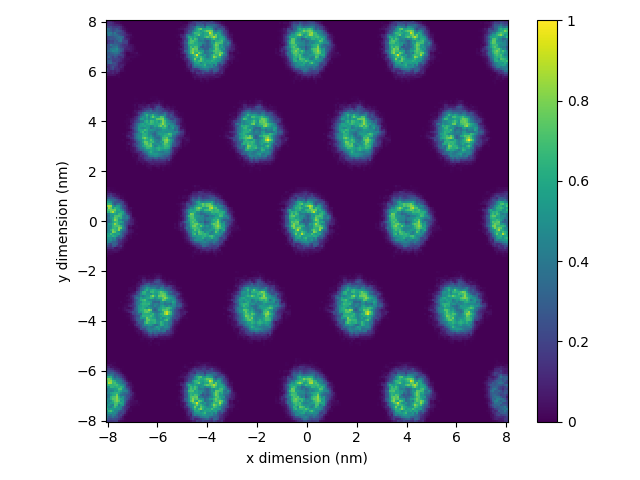
\includegraphics[width=\linewidth]{disorder_offset_xy_rings.png}
                \caption{}~\label{fig:disorder_offset_xy}
        \end{subfigure}
  \end{subfigure}
  \caption{}\label{fig:xy_correlation}
  \end{figure}

  The simulated X-ray diffraction patterns indicate further structural
  differences. In the parallel displaced configuration, almost all contrast
  between R-spots and R-alkanes fades (Fig.~\ref{fig:offset_disordered_xrd}). In
  the sandwiched configuration, R-spots is weakly present, but in different
  locations, showing higher intensity at the top and bottom of the pattern as
  well as at the intersection of R-alkanes with q$_z$ = 0 (Fig.
  ~\ref{fig:layered_disordered_xrd}). 

  The sandwiched and parallel displaced assemblies do not deviate from their
  initial head group arrangement. R-helix is still faintly visible in the
  parallel displaced configuration and is absent in the sandwiched simulated
  diffraction pattern. The spectroscopic signatures are unique to the two
  different head group configurations.

  The equilibrated pore spacing and distance between layers are different in
  the disordered pore basin. For both head group stacking arrangements, we
  observe a decrease in pore spacing (Fig.~\ref{fig:p2p_disordered}) and a
  corresponding increase in the equilibrated distance between layers
  (Fig.~\ref{fig:dbwl_disordered}). 

  \begin{figure}[!hbt]
        \centering
        \begin{subfigure}{0.45\linewidth}
                \centering
                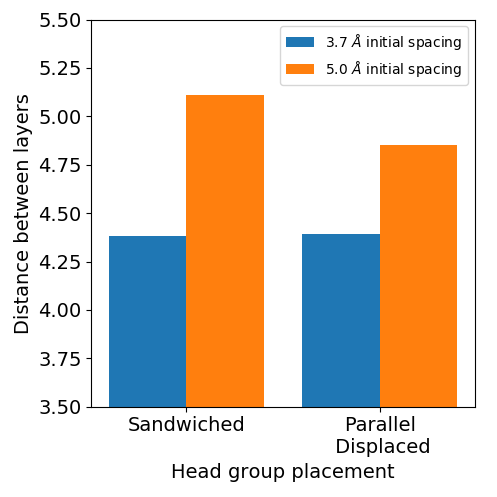
\includegraphics[width=\linewidth]{dbwl.png}
                \caption{}~\label{fig:dbwl_disordered}
        \end{subfigure}%
        \begin{subfigure}{0.45\linewidth}
                \centering
                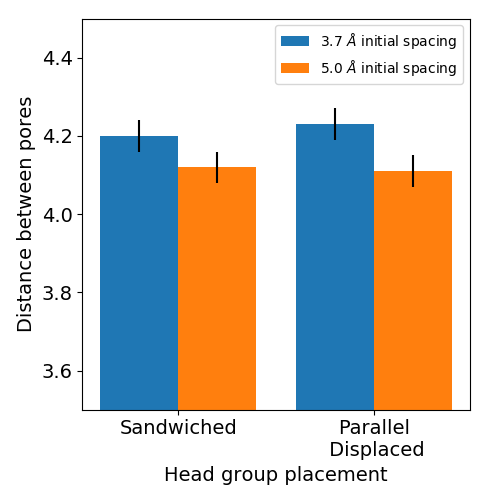
\includegraphics[width=\linewidth]{p2p2.png}
                \caption{}~\label{fig:p2p_disordered}
        \end{subfigure}
        \begin{subfigure}{0.45\linewidth}
                \centering
                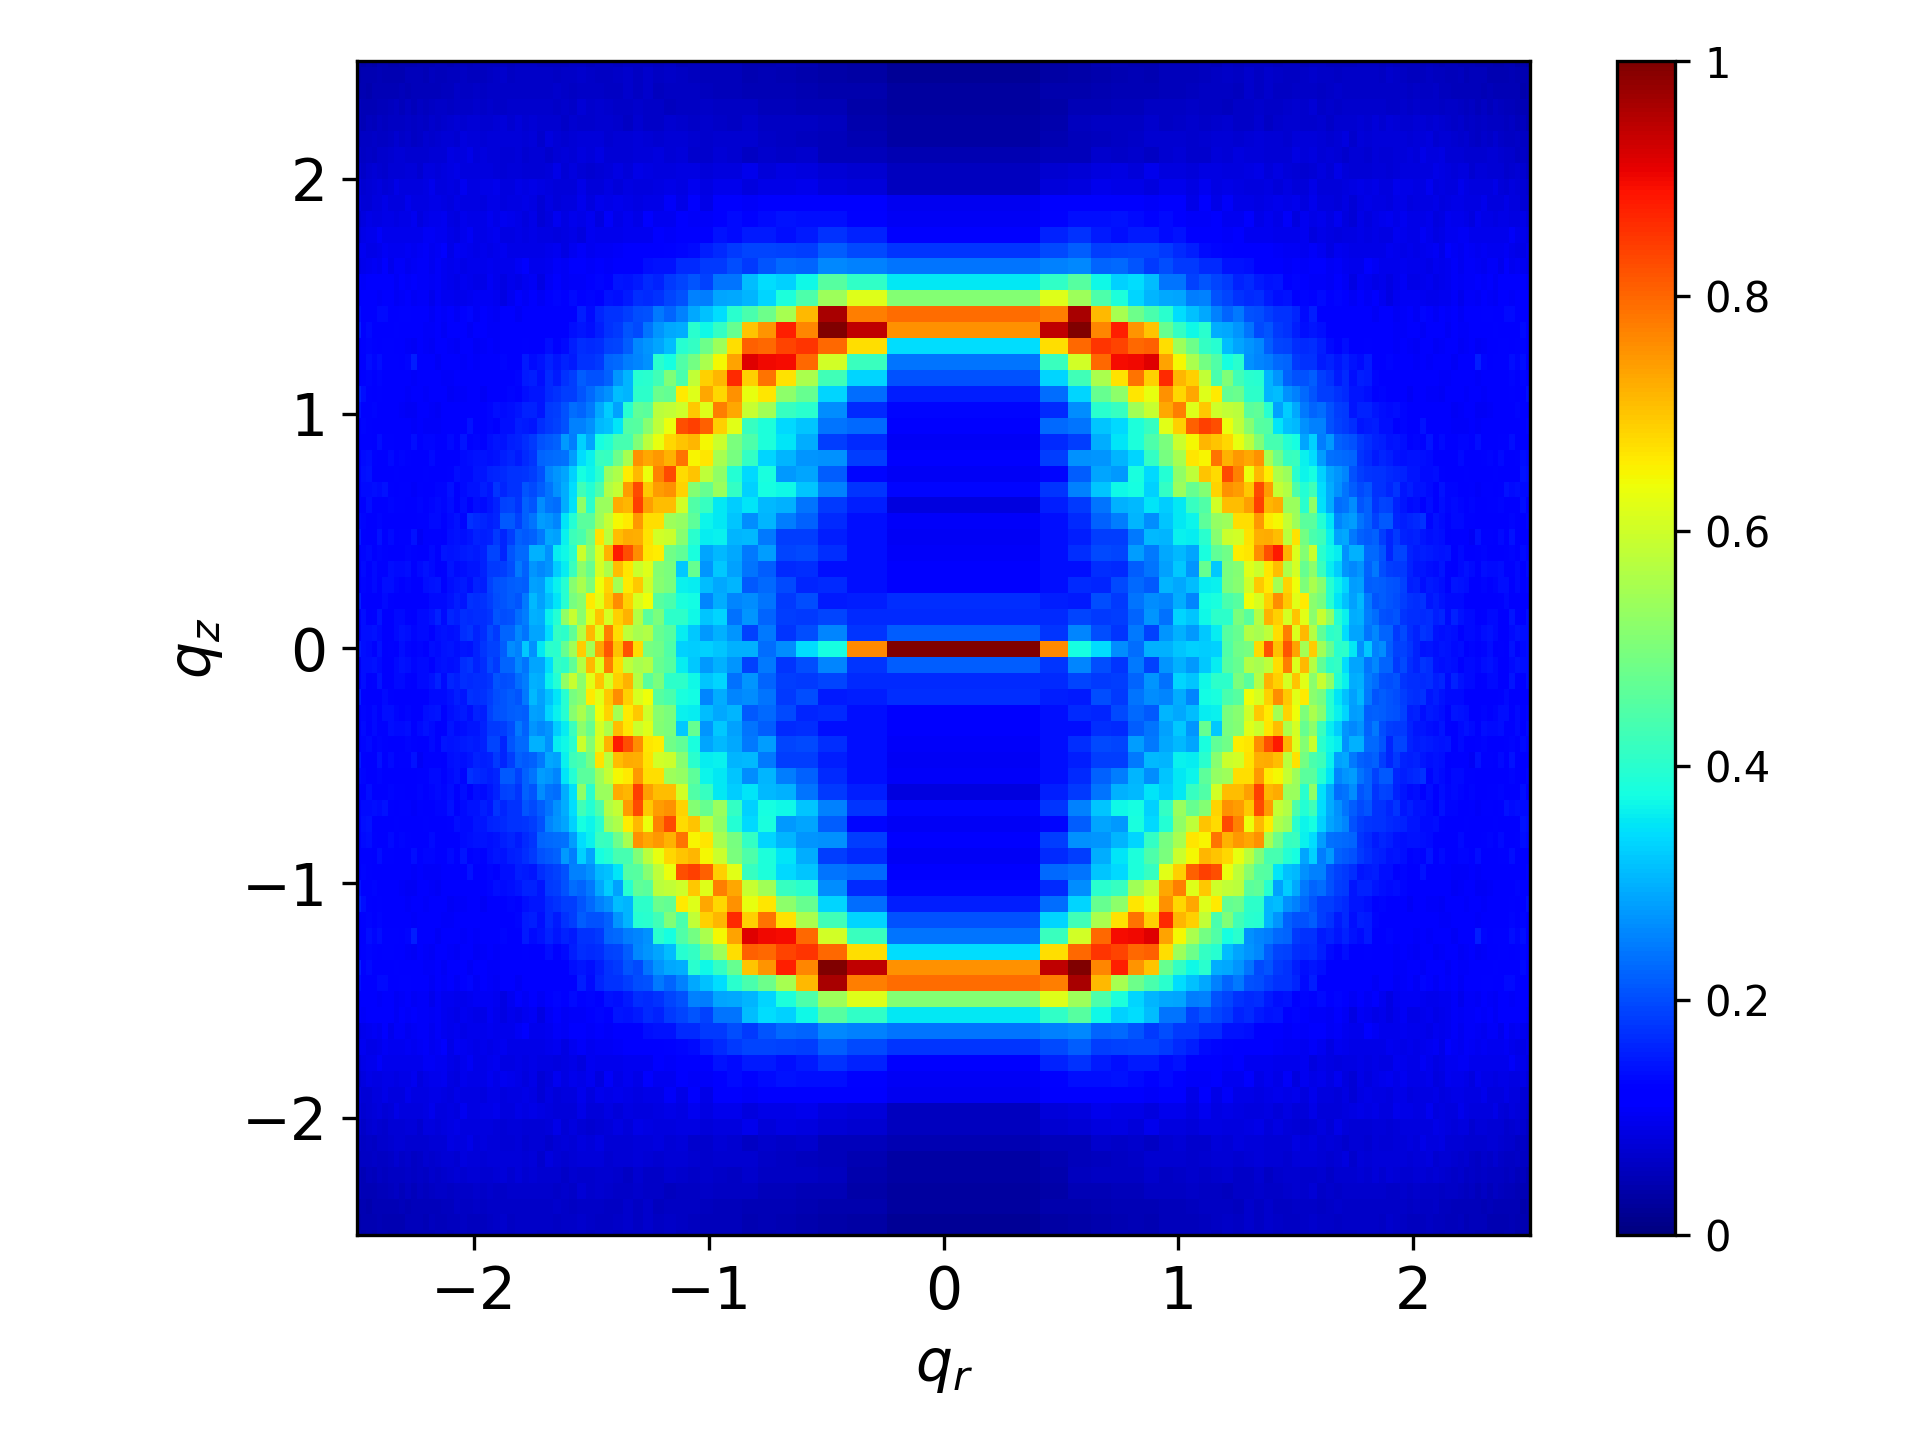
\includegraphics[width=\linewidth]{offset_disordered_rzplot.png}
                \caption{}~\label{fig:offset_disordered_xrd}
        \end{subfigure}%
        \begin{subfigure}{0.45\linewidth}
                \centering
                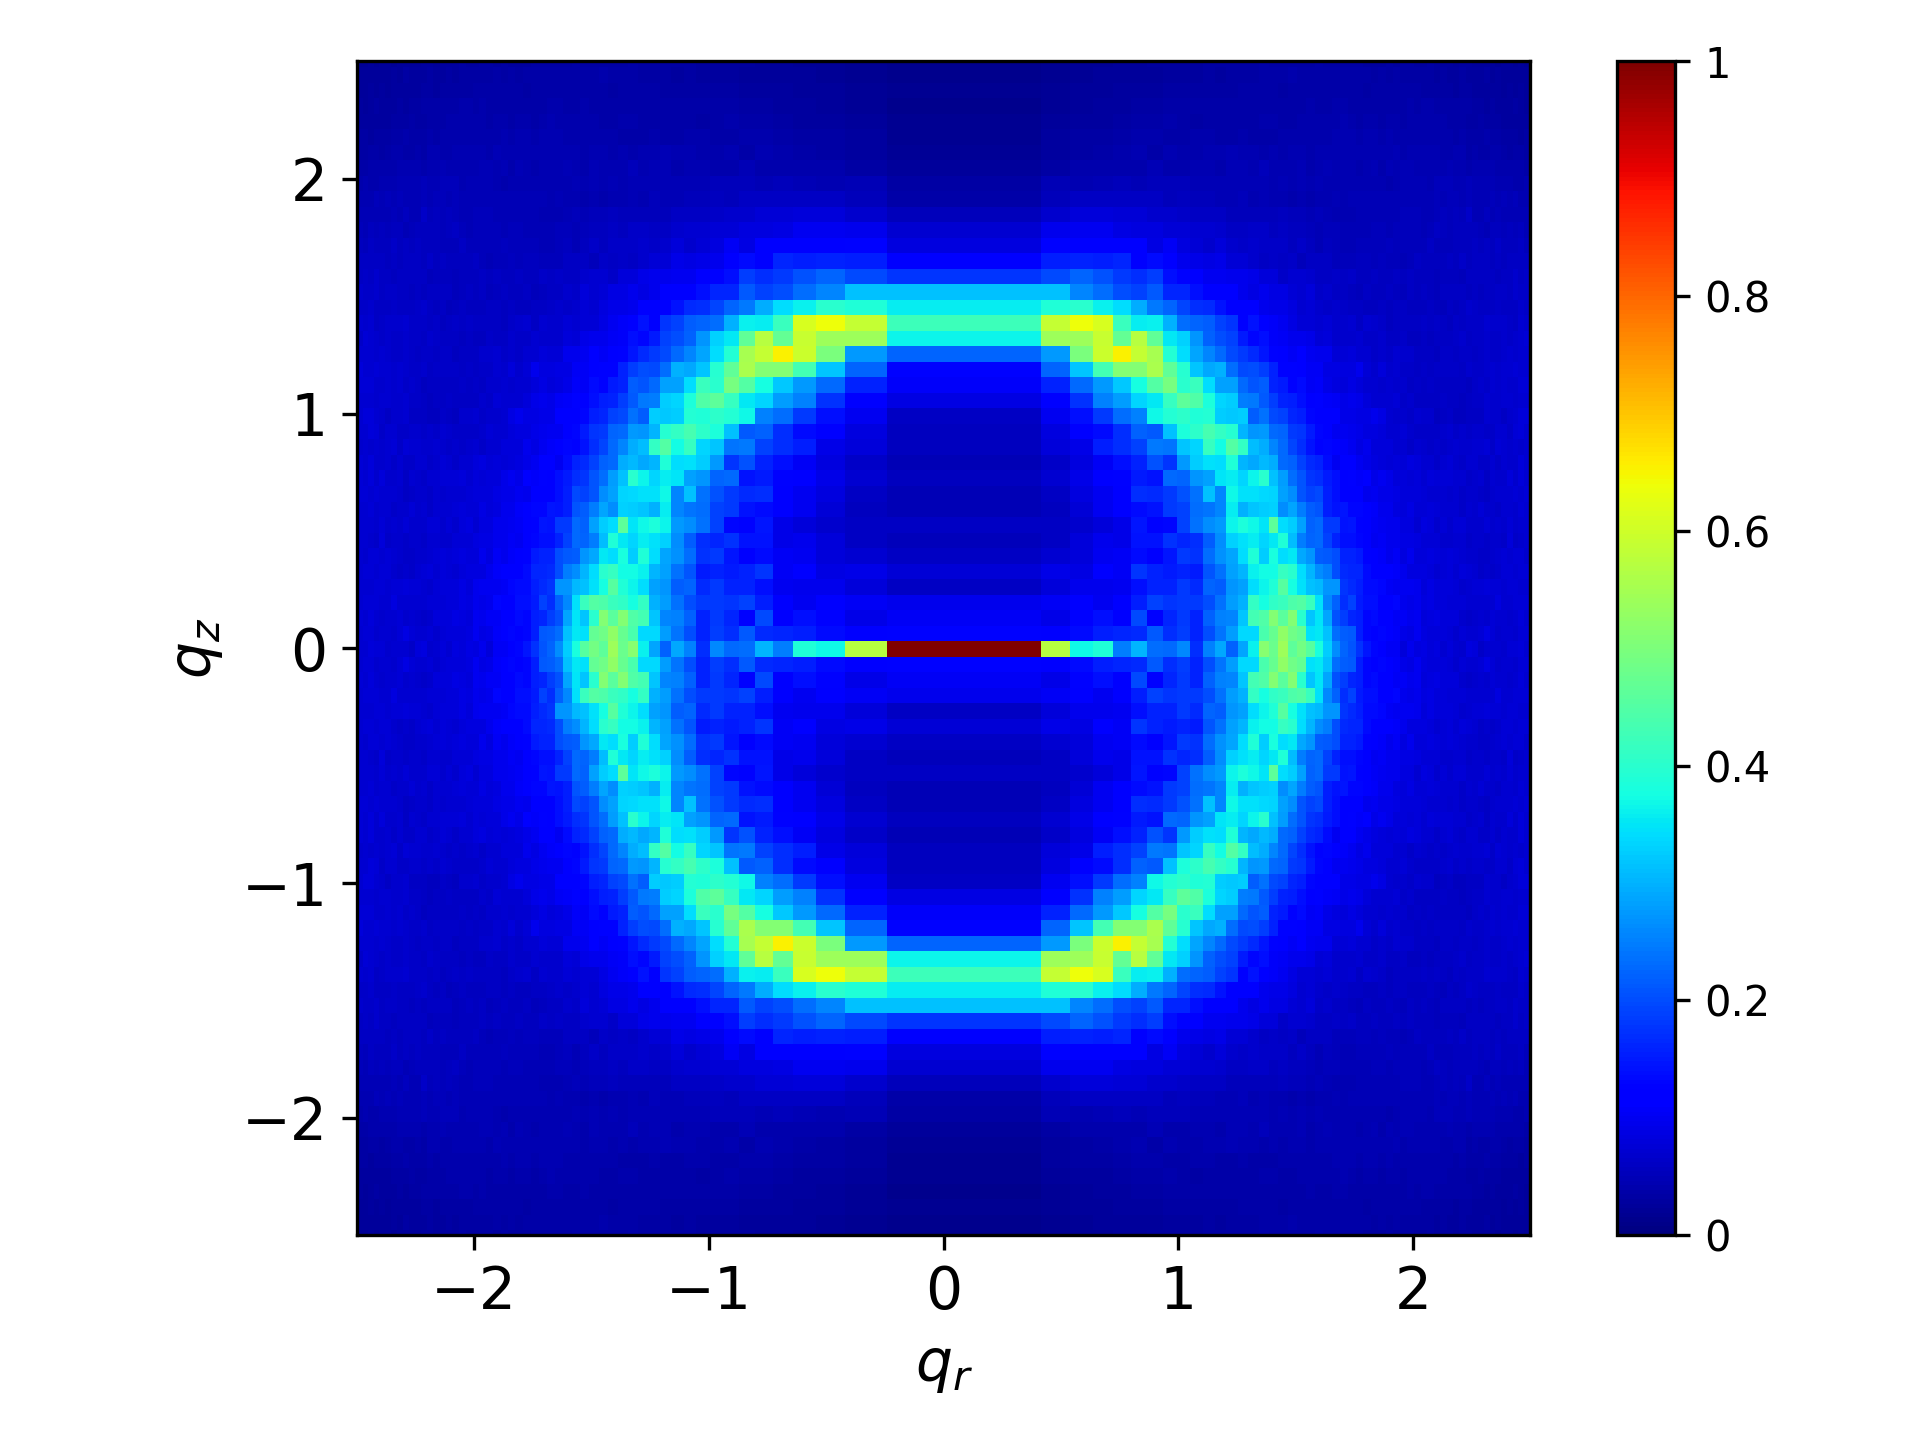
\includegraphics[width=\linewidth]{layered_disordered_rzplot.png}
                \caption{}~\label{fig:layered_disordered_xrd}
        \end{subfigure}
	\caption{There are distinct differences between the disordered and ordered pore systems. 
		When layers are initially stacked 5\AA~ apart, the distance
		between layers increases (a) and the pore spacing decreases (b) in comparison to
		the ordered pore systems. The simulated
		XRD patterns of disordered pore systems are also appreciably different, most 
		notably in the region bounded by R-alkanes. The disordered pore
		systems started in the parallel displaced configuariton (c) does not show R-spots
		or R-$\pi$ which suggests that head groups are not associating with each other
		and tails are distributed nearly isotropically. The disordered pore system
		started in the sandwiched configuration (d) does not show R-$\pi$ but R-spots 
		is present in different locations because the tails are packed in a different
		motif.}
  \end{figure}

  \subsection{Pore Composition Depends on Initial Configuration}

  In order to address (\ref{point:poredefinition}), we plotted the number
  densities of heavy atoms in the head group, carbon atoms in the tail region
  and the sodium ions (Figure~\ref{fig:densities}). For the head group region,
  we used the carbon atoms making up the aromatic ring. For the tail region we
  used only carbon atoms of the monomer tails (See Supplemental Information for
  diagram). We average the histograms over at least 50 ns of equilibrated trajectory.

  In all cases, the space in the pore region is filled with sodium ions and
  head groups. In the ordered pore systems, there is less density in the center of
  the pore indicating a more ordered pore structure. In both the sandwiched and
  parallel displaced configurations, we see the density of head groups and sodium
  ions fall to less than 50\% of its maximum at r = 0
  (Fig.~\ref{fig:layered_density}). The situation is most pronounced in the
  sandwiched configuration where the maximum head group density occurs 0.44 nm
  from the pore center. The parallel displaced configuration reaches its maximum
  0.35 nm from the pore center. In contrast, both disordered pore systems show
  very little difference in density from its maximum. This implies a more uniform
  distribution of head groups within the pore center. 
  % High vacancy is less likely to be stable in the real system

  There is a partition between the hydrophobic and hydrophilic regions, however
  it is a gradient in composition, rather than an abrupt division. The system
  does not confine sodium ions and head groups to just within the pore region.
  Assuming a pore radius of 0.6 nm, we see in all cases, that 19\% of sodium ions
  exist outside the pore region (except sandwiched, ordered pore, where 16\%
  are outside the pore). Additionally, we see that in all cases, about 3\% of the
  plotted tail density is located within the pore region (except sandwiched,
  ordered pore, where 1.5\% are within the pore region). These observations bring
  into question how one should define a pore in these types of systems. One
  usually measures a membrane's pore radius based on the size of a molecule it
  can reject, however it is not clear where the edges of the pores are and what
  size molecule would fit through. We leave these investigations for a future
  study.

  \begin{figure}
  \centering
  \begin{subfigure}{0.45\textwidth}
        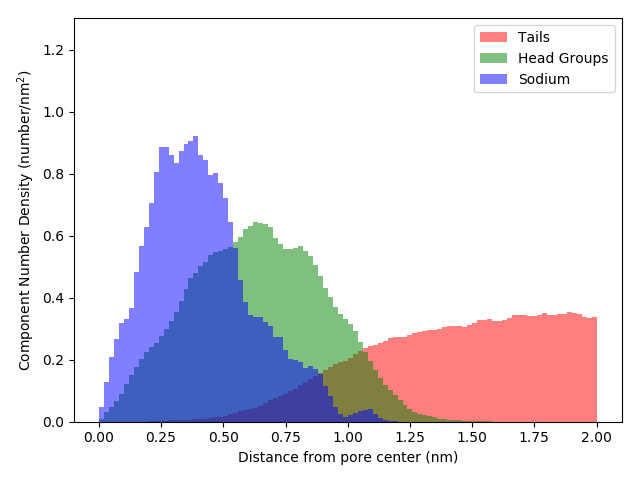
\includegraphics[width=1\linewidth]{offset_density.png}
        \caption{Parallel displaced, 3.7 \AA~initial layer spacing}
        \label{fig:offset_density}
  \end{subfigure}
  \begin{subfigure}{0.45\textwidth}
        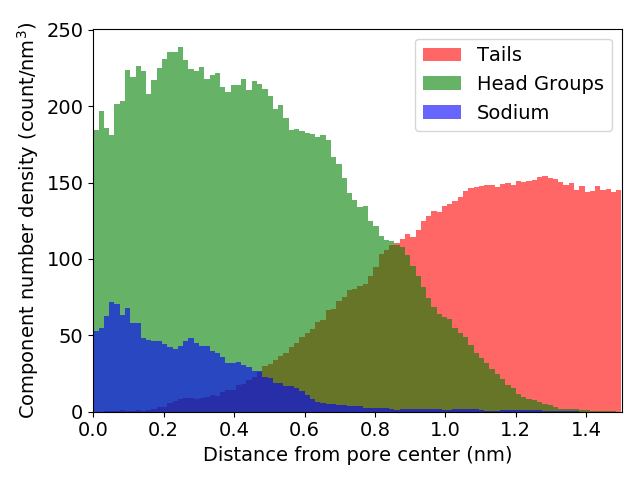
\includegraphics[width=1\linewidth]{layered_density.png}
        \caption{Sandwiched, 3.7 \AA~initial layer spacing}
        \label{fig:layered_density}
  \end{subfigure}
  \begin{subfigure}{0.45\textwidth}
        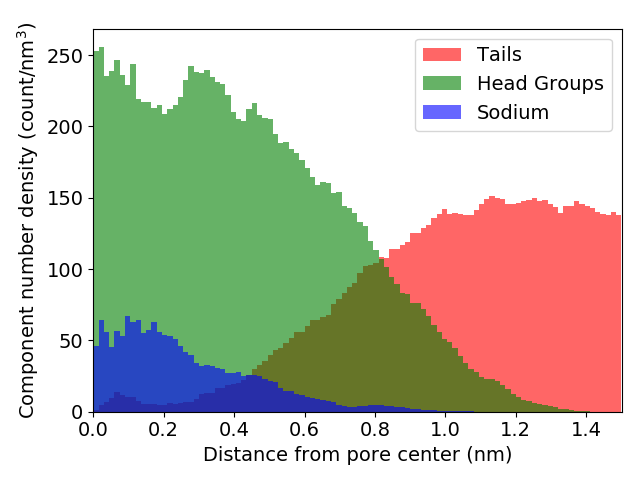
\includegraphics[width=1\linewidth]{disordered_offset_density.png}
        \caption{Parallel displaced, 5 \AA~initial layer spacing}
        \label{fig:disordered_offset_density}
  \end{subfigure}
  \begin{subfigure}{0.45\textwidth}
        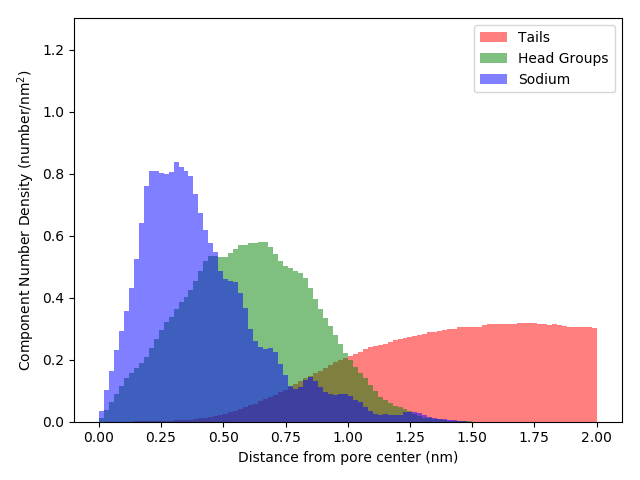
\includegraphics[width=1\linewidth]{disordered_density.png}
        \caption{Sandwiched, 5 \AA~initial layer spacing}
        \label{fig:disorder_layered_density}
  \end{subfigure}
  \caption{In all cases, the component radial distribution functions exhibit a
	  composition gradient transitioning from the hydrophilic to the hydrophobic
	  regions. Systems with layers initially spaced 3.7 \AA~apart in the  parallel
	  displaced (a), and sandwiched (b) configurations both show the highest
	  concentrations of ions and head groups away from the pore center. Systems with
	  layers initially spaced 5 \AA~apart (c) and (d), both show the highest
	  concentrations of ions and head groups near the pore center, implying a more
	  uniform, disordered pore.}~\label{fig:densities}
  \end{figure}

  \subsection{Affect of Water on Structure}

  We explored the affect of water on pore structure, addressing (\ref{point:water})
%  We answered (\ref{point:water}) and further support (\ref{point:orientation})
  by preparing parallel displaced and sandwiched configurations according to the
  wet equilibration procedure. There is no experimental measurement of trace
  water concentration in the pores so we tested a range of water concentrations
  from 0.5 to 5 percent. Our lower bound models a system with on average 2 water
  molecules for each monomer layer. Figure~\ref{fig:solvation} shows the
  simulated diffraction patterns resulting from each configuration.

  % formatting taken from : https://tex.stackexchange.com/questions/239715/add-titles-for-rows-and-columns-in-a-subfloat
  \newlength{\tempdima}
  \newcommand{\rowname}[1]% #1 = text
  {\rotatebox{90}{\makebox[\tempdima][c]{\textbf{#1}}}}
  
  \renewcommand{\thesubfigure}{\alph{subfigure}}
  \newcommand{\mycaption}[1]% #1 = caption
  {\refstepcounter{subfigure}\textbf{(\thesubfigure) }{\ignorespaces #1}}
  
  \begin{figure}
  	\settoheight{\tempdima}{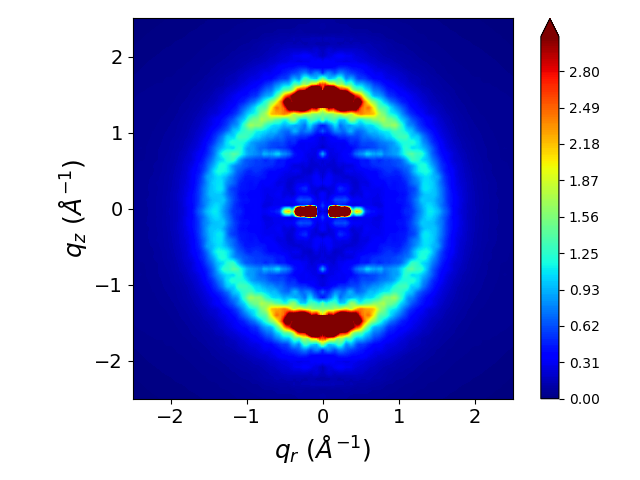
\includegraphics[width=.32\linewidth]{solvated_offset_rzplot_1.png}}%
  	\centering\begin{tabular}{@{}c@{ }c@{ }c@{ }c@{}}
  	&\textbf{1 wt\%} & \textbf{\hspace{2em}2.5 wt\%} & \textbf{5 wt\%} \\
  	\rowname{Parallel Displaced}&
  	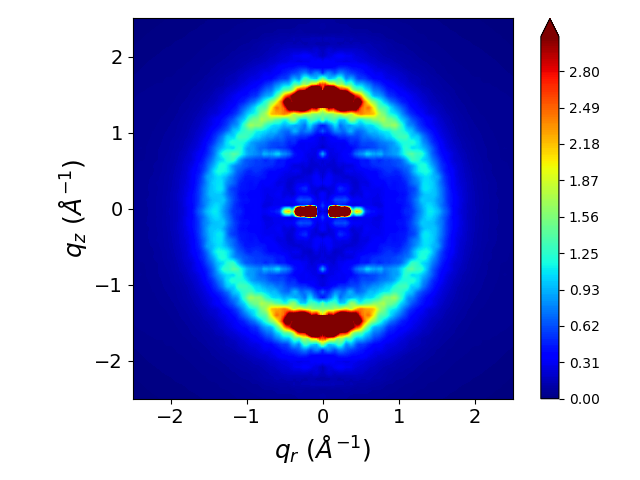
\includegraphics[width=.28\linewidth]{solvated_offset_rzplot_1.png}&
  	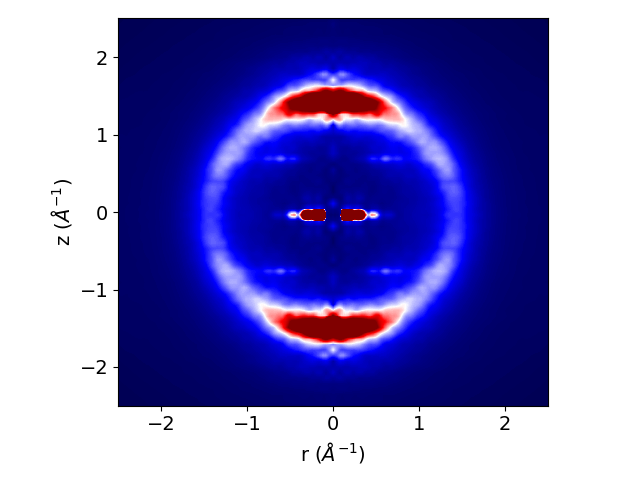
\includegraphics[width=.28\linewidth]{solvated_offset_rzplot_25.png}&
  	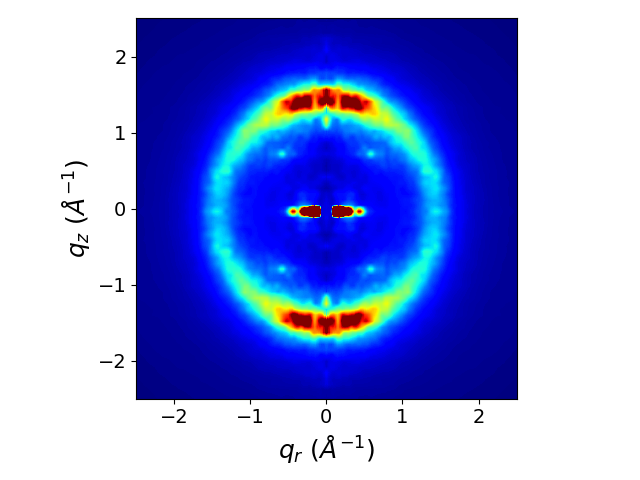
\includegraphics[width=.325\linewidth]{solvated_offset_rzplot_5.png}\\[-1ex]
  	%&\mycaption{0.2} & \mycaption{0.2} & \mycaption{0.3}\\
  	\rowname{Sandwiched}&
  	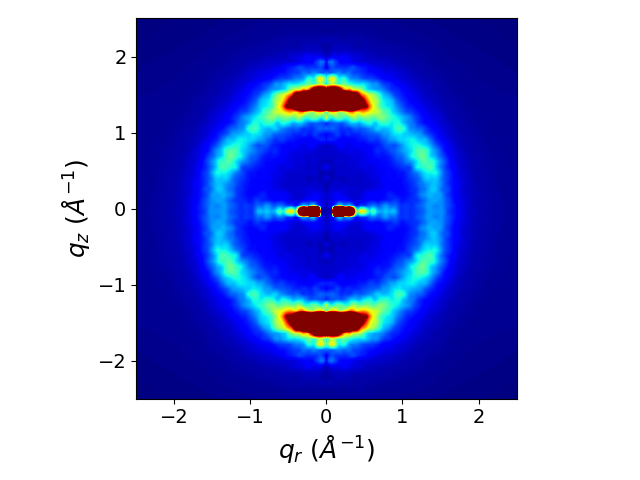
\includegraphics[width=.28\linewidth]{solvated_layered_rzplot_1.png}&
  	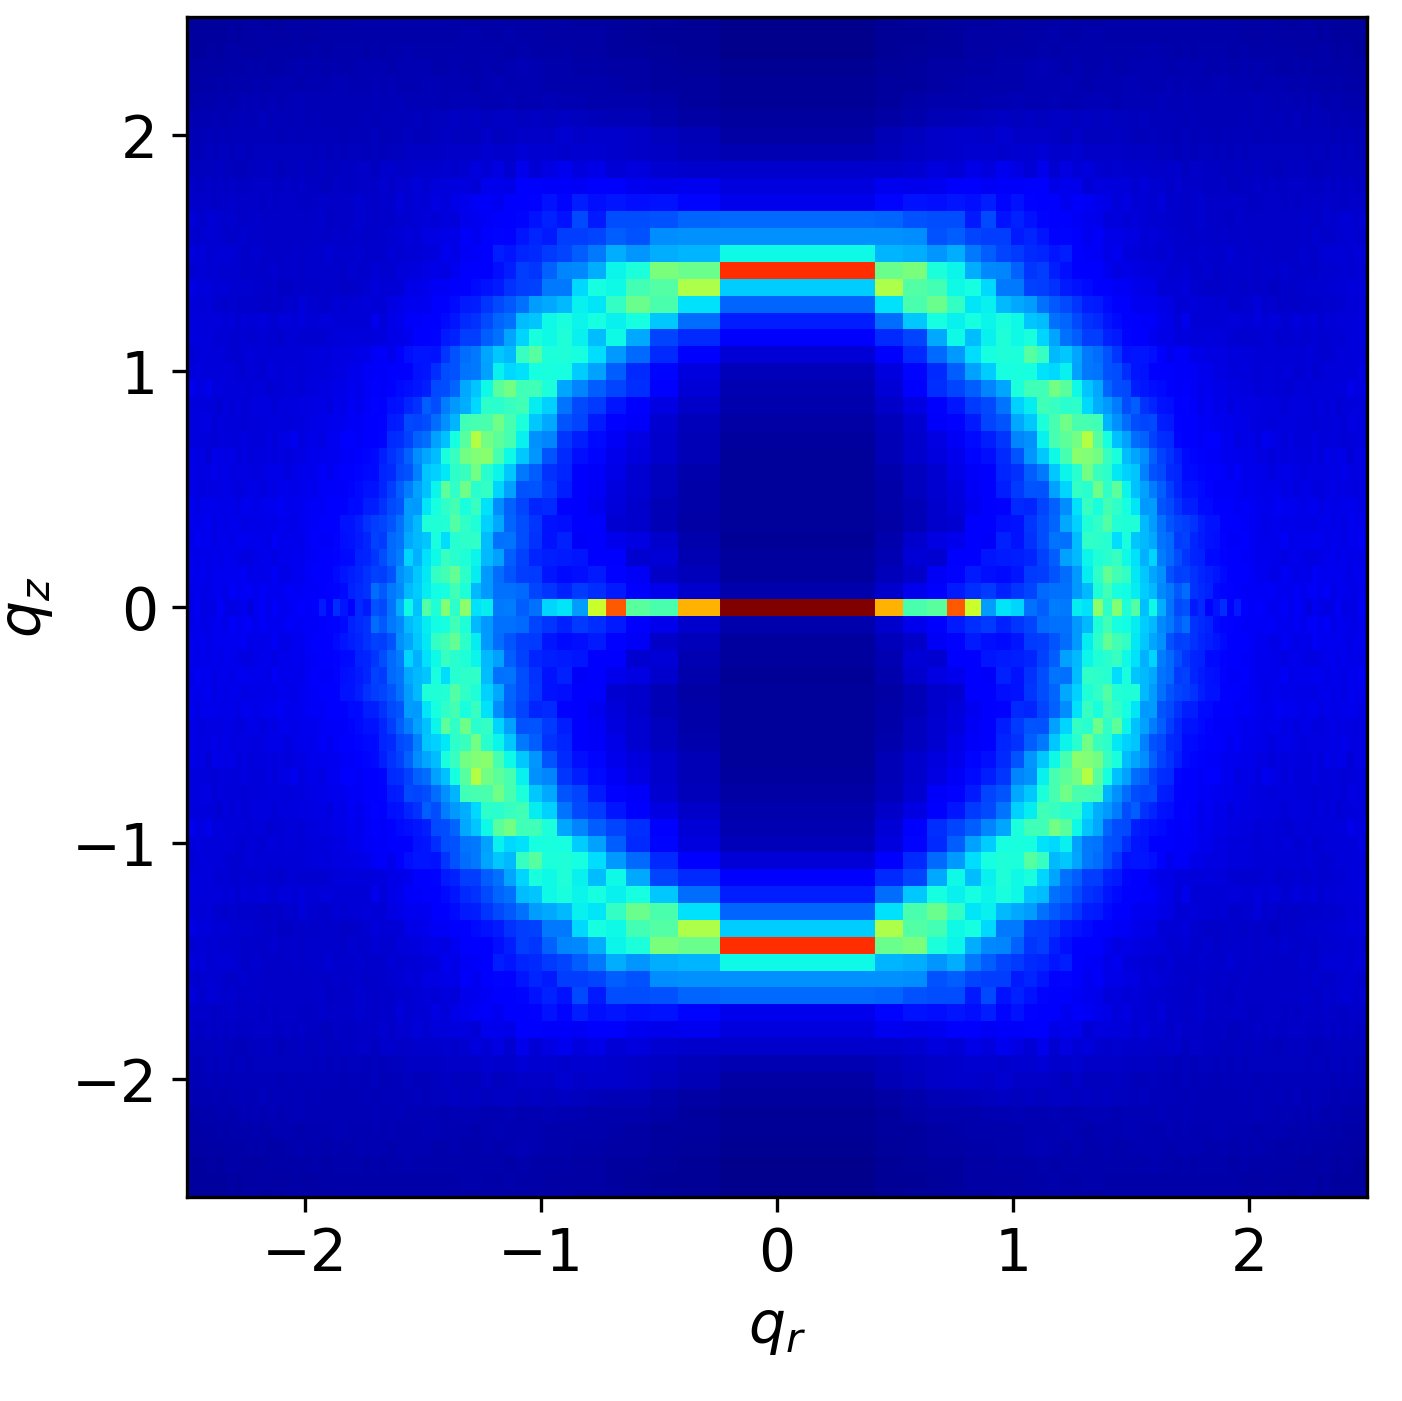
\includegraphics[width=.28\linewidth]{solvated_layered_rzplot_25.png}&
  	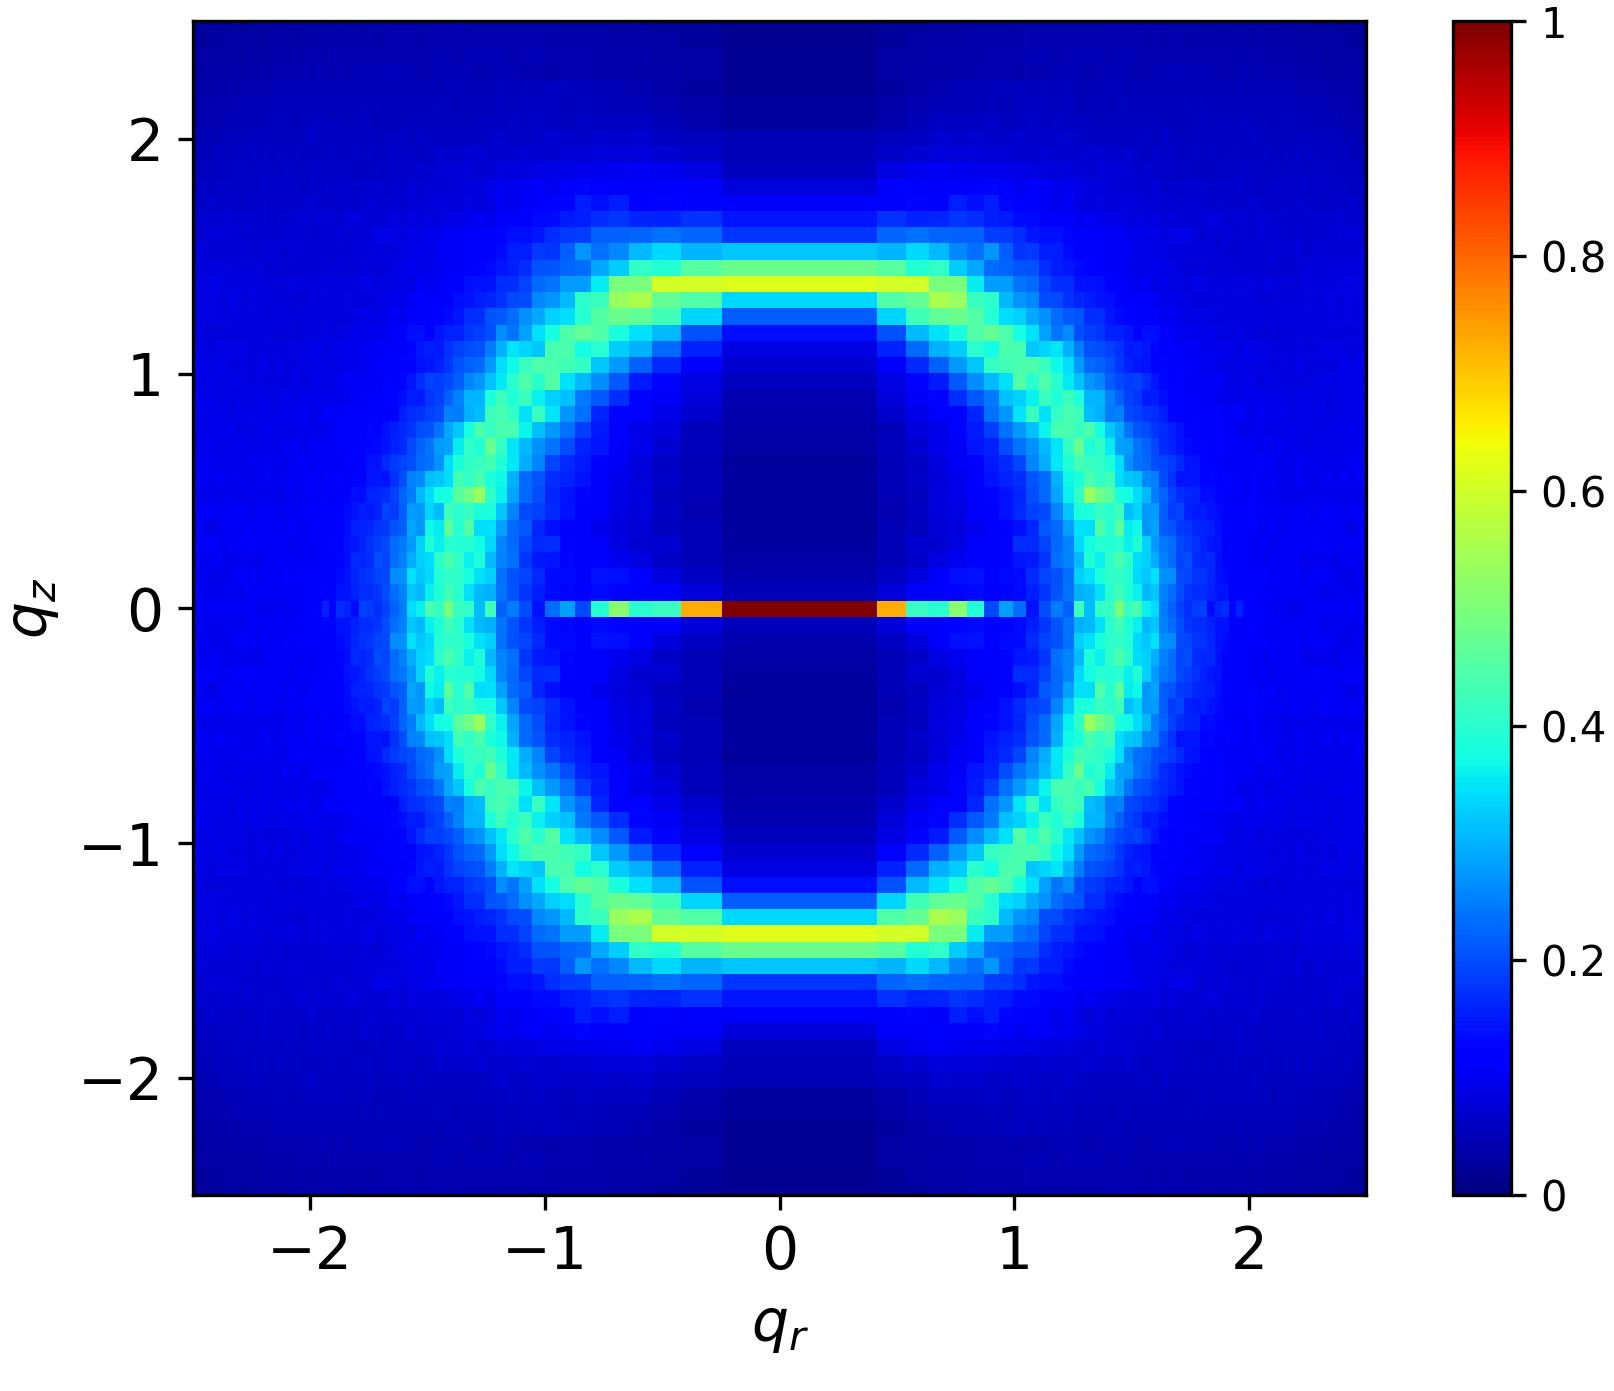
\includegraphics[width=.325\linewidth]{solvated_layered_rzplot_5.png}\\[-1ex]
  	%\mycaption{0.5} & \mycaption{0.6} & \mycaption{0.7} \\
  	\end{tabular}
	\caption{Simulated XRD patterns indicate that systems with added water
		are not as structured as the dry systems. As increasing amounts of water are 
		added to both systems, R-$\pi$ fades. When 2.5 wt\% water is added to the
		sandwiched system, R-$\pi$ gains back some intensity, but its magnitude is not
		greater than the dry system. R-spots also disappears as water is added. It is
		absent in all parallel displaced simulations, but fades gradually as water is
		added to the sandwiched configuration.}%
  \label{fig:solvation}

  \end{figure}
 
  In all cases, water disrupts structuring of the model \ref{fig:solvation}.
  When we add water to the system, the intensity of the reflections decrease. In
  systems built with 5 wt\% water, R-$\pi$ and R-spots become nearly
  indistinguishable from R-alkanes.

  % BJC: unsure where or if this paragraph fits
  Water is not necessary to maintain an ordered pore structure. We do not
  eliminate the possibility that water is necessary in order to drive
  self-assembly, but studying the mechanisms of self-assembly is beyond the
  scope of this work. According to our model, once the system has formed the
  Col\textsubscript{h} phase, adding water only drives disorder of the pore
  structure. In the true equilibrium configuration, if water exists, it is
  primarily confined to the pore region where there is no driving force for
  aggregation of water molecules. In the case of trace water, water molecules
  will be too sparse to form a hydrogen bonding network.

  In systems built with 5 wt\% water, the pore region becomes filled with
  water. We plotted the number density of components in this system. As with the 
  dry systems, we see a gradual compositional transition from hydrophilic to hydrophobic.  
  We see that the pores become a mixture of water molecules and sodium ions (Fig.
  \ref{fig:water_density}). 
  
  The membrane swells when we introduce water. The location of maximum head
  group density shifts from 0.35 to 0.62 nm and from 0.44 to 0.61 nm in the
  parallel displaced and sandwiched configurations respectively. Again, we
  observe the existence of ions, head groups and water outside the pore region,
  however in the hydrated system, the head groups drift beyond 1.5 \AA~from the
  pore center. In the dry systems, head groups did not wander beyond 1.4 \AA~from
  the pore center. Both observations suggest that water pushes all components
  radially outward from the pore center, characteristic of a swelling process. 
   
  This system is a closer representation of the H\textsubscript{II} phase which
  is typically synthesized with ca. 8 wt\% water. Further investigation of
  hydrated systems can help unravel the mechanisms for selective transport in
  separations of aqueous solutions. 

  \begin{figure}
  \centering 
  \begin{subfigure}{0.45\textwidth}
        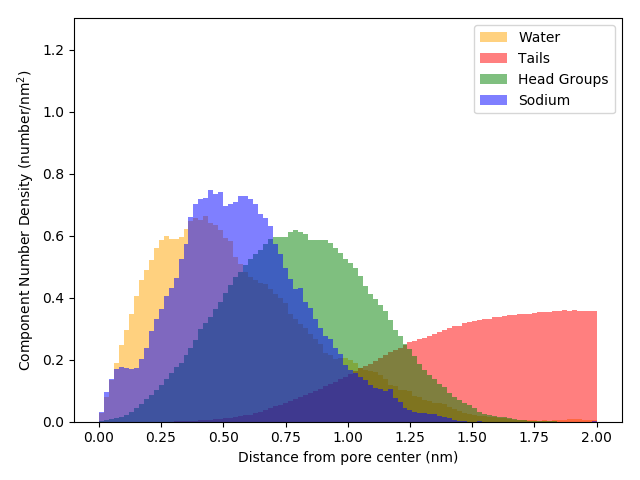
\includegraphics[width=1\linewidth]{offset_solvated_density.png}
        \caption{Parallel Displaced}
        \label{fig:offset_solvated_density}
  \end{subfigure}
  \begin{subfigure}{0.45\textwidth}
        \includegraphics[width=1\linewidth]{layered_solvated_density.png}
        \caption{Sandwiched}
        \label{fig:layered_solvated_density}
  \end{subfigure}
  \caption{Water fills the membrane pores in the parallel displaced (a) and
	  sandwiched (b) configurations. We define the pore region to be within 0.6 nm of
	  the pore center. Head groups in the sandwiched configuration sit closer to the
	  pore center than they do in the parallel displaced configuration. The parallel
	  displaced pores are composed primarily of water close to the pore center.}
  \label{fig:water_density}
  \end{figure}
  %MRS4: weird there's a head group peak in the center. Not enough statistics, so shot noise from the r^2 dr weighting?
  %BJC3: Yea, I'm not sure exactly. I'll look more into it. It might one or two head groups that just get stuck there.
  % The pore I picture in the supplemental info is completely cleared of any head groups. 

  \subsection{Model Ionic Conductivity Measurements}

  We used the equilibrated parallel displaced system to calculate ionic
  conductivity since its structure is the closest match to experiment. The model
  gives reasonable estimates of ionic conductivity when compared to experiment.
  We compare calculated values of ionic conductivity obtained using the
  Nernst-Einstein relation and Collective Diffusion model in
  Figure~\ref{fig:conductivity}. The two methods agree with each other within
  error, although the uncertainty obtained using the Collective Diffusion model
  is much higher. We require much longer simulations to lower the uncertainty,
  however it is not feasible to do so with a large system. We will only use the
  Nernst-Einstein relation in future calculations of this type. 

  The calculated values of ionic conductivity are higher than experiment by an
  order of magnitude. One can justify the reason for this result by considering
  the real system studied experimentally. The ionic conductivity measurement to
  which we are comparing was done with a \SI{80}{\micro\metre} thick film, nearly
  10,000 times thicker than our simulated system. The thick film is likely
  imperfectly aligned and has defects leading to non-contiguous pores. It has
  been shown that there is a large dependence of ionic conductivity on the
  alignment of the pores. The ionic conductivity of an unaligned film is ca. 85
  times lower than that of a nearly aligned film referenced here. We hypothesize
  that a thin, perfectly aligned film would have a value of ionic conductivity in
  closer agreement with our model.
 
  \begin{figure}
        \centering
        \includegraphics[width=0.5\linewidth]{IC_offset.png}
        \caption{The collective diffusion model and the nernst-einstein relation yield
        agreeing values of ionic conductivity. Both methods give calculated
        values of ionic conductivity an order of magnitude higher than the experimental
        value.}
        \label{fig:conductivity}
  \end{figure}

  \subsection{Effect of Crosslinking}\label{section:xlink}

  The system's structure and physical characteristics did not change
  significantly when we applied the cross-linking algorithm to the equilibrated
  parallel-displaced configuration built with 5 monomers per layer. We simulated
  the cross-linked system in the NPT ensemble for 100 ns. After the system is
  cross-linked, the distance between pores shrinks by 0.4 \AA~and the distance
  between layers increases by 0.04 \AA. All major features are still present in
  the simulated XRD patterns, however at lower intensities
  (Fig.~\ref{fig:rzplot_xlink}). We calculated the ionic conductivity using the
  Nernst-Einstein relation and found that it is lower in the cross-linked system
  (Fig.~\ref{fig:IC_xlink}).

  %BJC: add units
  \begin{figure}
  \centering
  \begin{subfigure}{0.45\textwidth}
	\centering
	\includegraphics[width=\textwidth]{rzplot_xlink.png}
	\caption{}~\label{fig:rzplot_xlink}
  \end{subfigure}
  \begin{subfigure}{0.45\textwidth}
	\centering
	\includegraphics[width=\textwidth]{IC_xlink.png}
	\caption{}~\label{fig:IC_xlink}
  \end{subfigure}
  \begin{subfigure}{0.45\textwidth}
	\centering
	\includegraphics[width=\textwidth]{dbwl_xlink.png}
	\caption{}~\label{fig:dbwl_xlink}
  \end{subfigure}
  \begin{subfigure}{0.45\textwidth}
	\centering
	\includegraphics[width=\textwidth]{p2p_xlink.png}
	\caption{}~\label{fig:p2p_xlink}
  \end{subfigure}
  \caption{Applying our simulated crosslinking mechanism to an equilibrium
	  configuration causes slight changes to the system's physical and structural
	  properties. (a) Reflections produced by the cross-linked configuration are
	  faded relative to the uncross-linked system. (b) The ionic conductivity is
	  smaller relative to the uncross-linked system, but still much larger than the
	  experimental value. When the system is cross-linked, the distance between
	  layers increases (c) and the pore spacing decreases (d)}~\label{fig:xlink}
  \end{figure}
 
  \section{Conclusion}
  
  We have used a detailed molecular model of the Col\textsubscript{h} phase
  formed by Na-GA3C11 in order to study its nanoscopic structure. While there
  have been efforts to model formation of various liquid crystalline phases with
  molecular dynamics, to our knowledge there have been no studies which attempt
  to examine their structure with the same level of detail presented here.

  Evidence strongly supports that monomers stay partitioned into layers which
  stack to create pores and that each layer contains 5 monomers. We see periodic
  spacing of layers based on the z-direction correlation function, $g(z)$ of
  atoms in the tails and separately of atoms in the head groups.  Systems not
  built with 5 monomers per layer result in assemblies whose pore-to-pore spacing
  is inconsistent with experiment. 

  We have explored the affect of two different $\pi$-$\pi$ stacking modes on
  the equilibrated membrane structure. Simulated diffraction patterns generated
  from MD trajectories suggest that the parallel-displaced configuration produces
  a structure with the closest match to experiment.

  We have observed a number of metastable configurations. We witnessed
  long-term stability of systems built with a varied number of monomers per layer
  as well as in different $\pi$-$\pi$ stacking configurations. We also examined
  how the structure changes based on the initial distance between layers and
  showed how systems differ when built with layers spaced 5~\AA~versus
  3.7~\AA~apart. The configuration that showed the greatest agreement with
  experiment was built in the parallel-displaced configuration, with 5 monomers
  per layer and an initial layer spacing of 3.7 \AA.  
  % MRS4: do we have a sense of how consistent this behavior is? I.e. if
  % started with 4 apart does it look like 3.7 or 5 separations? How about 4.5?
  % Is there a gradual range of changes? Can we rule this out? What work was
  % done on this?
  % BJC3: I'll get back to you

  We characterized the environment centered around the membrane pores and
  learned that the pores are generally filled by monomer head groups and sodium
  ions. Membranes prepared in the sandwiched configuration have lower density 
  pores. We also observed that there is not a hard partition between hydrophlic
  and hydrophilic regions, rather there is a gradient.  This finding has raised
  questions about the nature of any size-exclusion separations.  

  We learned that we do not need water to create well-defined pore structures.
  Systems whose pores were filled with varying amounts of water showed a decrease
  in structuring relative to dry systems. 

  We justified that our system can reasonably estimate ionic conductivity.  Our
  calculations are about 1 order of magnitude higher than experiment, however
  that is to be expected since we are simulating a perfectly straight and
  defect-free membrane. 

  Finally, we verified that our conclusions do not change when the system is
  cross-linked by the algorithm we implemented. The diffraction pattern weakens
  relative to the uncross-linked system, the ionic conductivity drops by a factor
  of ca. 1.5, in closer agreement with experiment, the pore spacing decreases and
  the membrane becomes thicker. 

  With the structural understanding gained by these simulations, we will
  evaluate transport of various solutes within the system. We will apply the
  knowledge gained from this study in order to suggest improvements to the
  existing system as well as to evaluate new unsynthesized LLC systems.

  \clearpage
  \bibliography{llc}

\end{document}

% LocalWords:  Nanostructured desalination biorefinement solute RO NF bruggen
% LocalWords:  polydisperse diffusivity solutes BJC ultrafiltration nanometer
% LocalWords:  ionizable pretreatment Graphene solvated Na GA zhou resel feng
% LocalWords:  ca wt mesophases al crosslinking THF nanoporous PDMS nanopores
% LocalWords:  TODO svg eps atomistically counterion nanoscopic counterions XRD
% LocalWords:  WAXS headgroups initio metastable timescales acessible leached
% LocalWords:  SAXS alkane alkanes Antechamber bccsym molcharge QUACPAC Openeye
% LocalWords:  Gromacs berendsen timescale Packmol xyz hydrophlic xy pd tshaped
% LocalWords:  KJ NVT kJ Parrinello Rahman gmx solvate polymerization FRP FRPs
% LocalWords:  crosslink binned DC MSD subharmonic matplotlib GAFF's xrd llc ab
% LocalWords:  polarizable reconcilable screenshot crosslinked uncrosslinked AA
% LocalWords:  nanofiltration permeability interfacial diamine polysulfone der
% LocalWords:  trimesoyl immiscible polymerizes etching Osuji's nanostructured
% LocalWords:  Donnan modelling nanotubes monodispersity maruyama Zeolites Col
% LocalWords:  lyotropic thermotropic png kinetically colorbar gromacs hess dr
% LocalWords:  gimp disassociate pore's barostat racemic colorbars Nernst LLCs
% LocalWords:  entropic rzplot transitioning spoel github pymbar Yelk Glaser
